% ╔══════════════════════════════════════════════════════════════════════════════╗
% ║  Flood Inundation Mapping From Sentinel-1 SAR Using HAND-Guided Gating     ║
% ║  and Uncertainty Quantification                                             ║
% ║  DKU Signature Work  ·  Bouchra Daddaoui  ·  2026                          ║
% ║                                                                             ║
% ║  COMPILE: pdflatex terrainflood_uq_paper.tex (twice) then                  ║
% ║           bibtex terrainflood_uq_paper  then  pdflatex (twice more)        ║
% ║  Or upload the whole paper/ folder to Overleaf (pdfLaTeX engine).          ║
% ║  Figures are referenced from ../results/paper_figures/                     ║
% ║  Adjust \graphicspath if compiling from a different directory.              ║
% ╚══════════════════════════════════════════════════════════════════════════════╝

\documentclass[12pt,oneside]{report}

%─── Page geometry ─────────────────────────────────────────────────────────────
\usepackage[letterpaper, top=1in, bottom=1in, left=1.25in, right=1in]{geometry}

%─── Typography ────────────────────────────────────────────────────────────────
\usepackage[T1]{fontenc}
\usepackage[utf8]{inputenc}
\usepackage{lmodern}            % clean scalable fonts
\usepackage{microtype}          % improved justification

%─── Spacing ───────────────────────────────────────────────────────────────────
\usepackage{setspace}
\setstretch{1.5}                % 1.5 line spacing (DKU standard)

%─── Mathematics ───────────────────────────────────────────────────────────────
\usepackage{amsmath, amssymb, mathtools}
\usepackage{bm}                 % bold math symbols

%─── Graphics ──────────────────────────────────────────────────────────────────
\usepackage{graphicx}
\usepackage{subcaption}
\usepackage{float}
\graphicspath{
  {../results/paper_figures/}
  {../results/paper_remote_sensing_maps/}
  {../results/eval_D_full/figures/}
  {../results/eval_C_full/figures/}
  {../results/paper_remote_sensing_figures/}
  {../results/}
}

%─── Tables ────────────────────────────────────────────────────────────────────
\usepackage{booktabs}
\usepackage{multirow}
\usepackage{array}
\usepackage{tabularx}
\usepackage{longtable}
\usepackage{xcolor}
\usepackage{colortbl}
\definecolor{rowgray}{gray}{0.93}

%─── Captions ──────────────────────────────────────────────────────────────────
\usepackage[font=small, labelfont=bf, width=0.92\textwidth]{caption}

%─── Bibliography ──────────────────────────────────────────────────────────────
\usepackage[numbers, sort&compress, square]{natbib}
\bibliographystyle{unsrtnat}

%─── Hyperlinks ────────────────────────────────────────────────────────────────
\usepackage[
  colorlinks=true,
  linkcolor=black,
  citecolor=blue!60!black,
  urlcolor=blue!60!black,
  pdftitle={Flood Inundation Mapping From Sentinel-1 SAR Using HAND-Guided Gating
            and Uncertainty Quantification},
  pdfauthor={Bouchra Daddaoui}
]{hyperref}

%─── Headers / footers ─────────────────────────────────────────────────────────
\usepackage{fancyhdr}
\pagestyle{fancy}
\fancyhf{}
\fancyhead[R]{\small\itshape TerrainFlood-UQ $\cdot$ Daddaoui (2026)}
\fancyfoot[C]{\thepage}
\renewcommand{\headrulewidth}{0.4pt}
\fancypagestyle{plain}{\fancyhf{}\fancyfoot[C]{\thepage}
                        \renewcommand{\headrulewidth}{0pt}}

%─── Chapter/section style ─────────────────────────────────────────────────────
\usepackage{titlesec}
\titleformat{\chapter}[display]
  {\normalfont\large\bfseries\centering}
  {\MakeUppercase{\chaptertitlename}\ \thechapter}
  {0.5em}
  {\LARGE\MakeUppercase}
\titlespacing*{\chapter}{0pt}{20pt}{30pt}

%─── Algorithms ────────────────────────────────────────────────────────────────
\usepackage[ruled,linesnumbered]{algorithm2e}

%─── Inline enumeration ────────────────────────────────────────────────────────
\usepackage[inline]{enumitem}

%─── Convenience macros ────────────────────────────────────────────────────────
\newcommand{\IoU}{\mathrm{IoU}}
\newcommand{\ECE}{\mathrm{ECE}}
\newcommand{\AURC}{\mathrm{AURC}}
\newcommand{\HAND}{\mathrm{HAND}}
\newcommand{\etal}{\textit{et~al.}}

% Reduce widow/orphan lines
\widowpenalty=10000
\clubpenalty=10000

%═══════════════════════════════════════════════════════════════════════════════
\begin{document}
\pagenumbering{roman}

%══════════════════════════════════════════════════════════════════════════════
%  TITLE PAGE
%══════════════════════════════════════════════════════════════════════════════
\begin{titlepage}
\centering
\vspace*{1.0cm}
{\large Duke Kunshan University}\\[0.3cm]
{\large\itshape Signature Work in Computation and Design}\\[1.8cm]

{\LARGE\bfseries FLOOD INUNDATION MAPPING FROM\\[0.3cm]
SENTINEL-1 SAR USING HAND-GUIDED\\[0.3cm]
GATING AND UNCERTAINTY QUANTIFICATION}\\[2.5cm]

{\large by}\\[0.5cm]
{\large\bfseries Bouchra Daddaoui}\\[1.5cm]

\begin{tabular}{rl}
  Mentor: & Prof. Dongmian Zou, Ph.D.\\
          & Division of Natural and Applied Sciences\\[0.4cm]
  Program: & Signature Work\\
  Division: & Computation and Design
\end{tabular}\\[2.0cm]

{\large May 2026}\\[1.5cm]

\vfill
\begin{minipage}{0.80\textwidth}
\centering
\small
Submitted in partial fulfilment of the requirements for the
Bachelor of Science degree at Duke Kunshan University.\\[0.5em]
\textit{This work is supported by the DKU Signature Work Research Grant
programme and the Social Science Divisional Chair's Discretionary Fund.}
\end{minipage}
\end{titlepage}

%──────────────────────────────────────────────────────────────────────────────
%  APPROVALS PAGE
%──────────────────────────────────────────────────────────────────────────────
\newpage
\thispagestyle{plain}
\begin{center}
  {\large\bfseries APPROVALS}
\end{center}
\vspace{1em}

\noindent Mentor: Prof. Dongmian Zou, Ph.D., Division of Natural and Applied Sciences

\vspace{3em}
\noindent\rule{6cm}{0.4pt}\\
Signature \hspace{4cm} Date

%──────────────────────────────────────────────────────────────────────────────
%  TABLE OF CONTENTS
%──────────────────────────────────────────────────────────────────────────────
\newpage
\tableofcontents

\newpage
\listoffigures

\newpage
\listoftables

%══════════════════════════════════════════════════════════════════════════════
%  ABSTRACT
%══════════════════════════════════════════════════════════════════════════════
\newpage
\phantomsection
\addcontentsline{toc}{chapter}{Abstract}
\begin{center}
  {\large\bfseries ABSTRACT}
\end{center}
\vspace{0.8em}

Floods are the costliest and most widespread natural hazard globally, yet
deep learning flood-mapping systems trained on well-instrumented regions
routinely fail when deployed to geographically distinct areas, a pervasive
out-of-distribution generalisation challenge that limits operational utility.
We present \textit{TerrainFlood-UQ}, a physics-informed Siamese ResNet-34
architecture that integrates a Height Above Nearest Drainage (HAND)
attention gate $\alpha = \exp(-h/50)$ into a dual-branch SAR encoder,
explicitly suppressing flood predictions in terrain where inundation is
physically implausible.
The model is paired with Monte Carlo Dropout and test-time augmentation over
the D4 symmetry group for principled predictive uncertainty quantification.
Through a rigorous four-variant ablation study evaluated on the Sen1Floods11
Bolivia out-of-distribution test set (15 chips; 2.87 million valid pixels),
we demonstrate that the terrain gate alone improves Intersection over Union
by 22.1 percentage points over a SAR-only baseline ($\IoU_A = 0.408
\to \IoU_C = 0.662$), far exceeding the benefit of simply providing HAND as
an additional input channel (3.3~pp, Variant~B).
Temperature calibration reduces Expected Calibration Error by 79\%
($0.363 \to 0.078$).
Full-length retraining of the physics-gated architecture with Monte Carlo
Dropout achieves $\IoU = 0.724$, establishing a clear quantitative advantage
over the unsupervised Otsu baseline ($\IoU = 0.582$).
These findings demonstrate that encoding terrain drainage physics as an
architectural prior, rather than as a learned input feature, is a highly
effective strategy for robust out-of-distribution SAR flood segmentation,
with direct implications for satellite-based disaster response in data-scarce
regions.

\vspace{0.8em}
\noindent\textbf{Keywords:} SAR flood mapping; uncertainty quantification;
physics-informed deep learning; HAND attention gate; Sentinel-1;
out-of-distribution generalisation; Monte Carlo Dropout; temperature scaling;
population exposure estimation.

%──────────────────────────────────────────────────────────────────────────────
%  ACKNOWLEDGEMENTS
%──────────────────────────────────────────────────────────────────────────────
\newpage
\phantomsection
\addcontentsline{toc}{chapter}{Acknowledgements}
\begin{center}
  {\large\bfseries ACKNOWLEDGEMENTS}
\end{center}
\vspace{0.8em}

The author thanks Prof. Dongmian Zou, Ph.D., for scientific mentorship and
guidance throughout this project.
Computational resources were provided by the Duke Kunshan University
Computing Cluster (DKUCC).
Sentinel-1 SAR imagery was obtained via Google Earth Engine and the
Copernicus Open Access Hub.
The Sen1Floods11 benchmark was made publicly available by Bonafilia
\etal~\cite{bonafilia2020sen1floods11}.
MERIT Hydro digital elevation data~\cite{yamazaki2019merit} and WorldPop
gridded population estimates~\cite{stevens2015disaggregating} were used under
their respective open-access licences.
Support from the DKU Division of Natural and Applied Sciences through SELF,
SRS, and Signature Work programme grants is gratefully acknowledged.

%══════════════════════════════════════════════════════════════════════════════
%  MAIN BODY
%══════════════════════════════════════════════════════════════════════════════
\newpage
\pagenumbering{arabic}
\setcounter{page}{1}

%══════════════════════════════════════════════════════════════════════════════
\chapter{Introduction}
%══════════════════════════════════════════════════════════════════════════════

\section{Motivation}

Flooding is the natural hazard responsible for the greatest human displacement
and economic loss worldwide.
Over the two decades from 2000 to 2019, floods affected 1.65 billion people
and inflicted approximately \$650 billion in direct economic damages
\cite{undrr2020}.
Under accelerating climate change, extreme inundation events are projected to
intensify substantially across tropical and temperate latitudes
\cite{hirabayashi2013global, bloschl2019changing}, making near-real-time flood
mapping an increasingly critical component of disaster risk management
infrastructure.

Synthetic Aperture Radar imagery from Sentinel-1 has become the default
observational resource for operational flood mapping because its active
microwave pulses penetrate cloud cover and function in complete darkness
\cite{torres2012gmes, moreira2013tutorial}.
Open water registers as very dark in C-band backscatter due to specular
reflection, enabling flood detection even during the overcast conditions that
accompany major events \cite{mason2012near}.
Despite two decades of SAR flood mapping research, however, producing reliable
predictions outside the training region remains an unresolved problem.
Models trained on European events routinely generate false positives over
tropical floodplains, where vegetation structure and soil moisture create
different backscatter signatures.
This out-of-distribution (OOD) generalisation failure is not merely an academic
concern: it undermines precisely the deployments where automated mapping is most
urgently needed, namely in rapidly developing and data-scarce regions where
floods cause disproportionate harm.

\section{Physics as an Inductive Bias}

A fundamental insight motivating this work is that flood inundation is strongly
constrained by the geomorphology of the landscape.
Water accumulates in valley bottoms and along drainage networks; it cannot pool
significantly at elevations far above the nearest channel.
The Height Above Nearest Drainage index \cite{renno2008hand}, derived from
globally available digital elevation models, encodes this physical constraint
with precision.
Pixels at HAND $\approx 0$\,m occupy riparian valley floors with high prior
flood probability; pixels at HAND $> 50$\,m occupy ridges and hillslopes where
major inundation is physically implausible.
This prior is independent of regional radar characteristics and does not require
re-estimation for new deployment regions, making it an ideal physical anchor for
improving out-of-distribution generalisation.

The central research question of this work is whether encoding this terrain
constraint as an \emph{architectural prior} provides a stronger inductive bias
than supplying it as an additional learned input feature.
The answer, demonstrated through controlled ablation, is decisive.

\section{The Uncertainty Problem}

Even an accurate flood map offers limited operational utility without calibrated
uncertainty estimates.
Emergency managers need to know not only \emph{where} a model predicts flooding
but \emph{how confident} that prediction is, so they can direct field
verification resources, prioritise interventions in high-exposure uncertain
zones, and communicate probabilistic risk to affected communities.

Monte Carlo Dropout \cite{gal2016dropout} offers a computationally inexpensive
approximation to Bayesian inference that can be layered onto any
dropout-regularised network.
Whether it produces calibrated, actionable uncertainty estimates for pixel-level
flood segmentation is an open empirical question that this work investigates
systematically, including an unexpected failure mode that reveals a structural
interaction between physics-gated architectures and stochastic inference.

\section{Contributions}

This work makes five contributions.

\begin{enumerate}
  \item \textbf{HAND Attention Gate.}  We introduce a physics-informed
        attention gate $\alpha = \exp(-h/50)$, which multiplicatively modulates
        decoder feature maps using terrain drainage height, suppressing flood
        predictions in elevated terrain without hard thresholding or
        region-specific calibration.  This gate is globally valid by physical
        law rather than learned from data, and its interaction with the Siamese
        change-detection architecture has not previously been studied.

  \item \textbf{Controlled Ablation Study.}  We conduct a four-variant
        controlled ablation on a strictly held-out geography (Bolivia),
        providing the first systematic comparison of terrain-gating versus
        terrain-concatenation strategies for OOD SAR flood segmentation.

  \item \textbf{Uncertainty Quantification Pipeline.}  We implement and
        compare Monte Carlo Dropout and test-time augmentation over the D4
        symmetry group as uncertainty estimators, demonstrating that TTA
        substantially outperforms MC Dropout due to a novel structural
        failure mode in physics-gated architectures.

  \item \textbf{Population Exposure Framework.}  We couple flood predictions
        with WorldPop gridded population data to produce uncertainty-aware
        exposure estimates, demonstrating an end-to-end pipeline from raw
        Sentinel-1 imagery to actionable risk metrics.

  \item \textbf{Negative Results.}  We report and carefully analyse negative
        results, including an inverted uncertainty–error correlation under MC
        Dropout that is mechanistically attributable to gate-induced logit
        suppression.  Transparent reporting of failure modes is essential for
        the safe deployment of deep learning systems in high-stakes
        humanitarian applications.
\end{enumerate}

\section{Organisation}

Chapter~\ref{ch:related} reviews relevant literature.
Chapter~\ref{ch:data} describes the dataset, study design, and preprocessing
pipeline.
Chapter~\ref{ch:methods} details the architecture, training procedure, and
uncertainty framework.
Chapter~\ref{ch:experiments} presents experimental results.
Chapter~\ref{ch:discussion} interprets the findings and Chapter~\ref{ch:conclusions}
concludes.

%══════════════════════════════════════════════════════════════════════════════
\chapter{Background and Related Work}
\label{ch:related}
%══════════════════════════════════════════════════════════════════════════════

\section{SAR-Based Flood Detection}

The history of SAR flood mapping is in many respects the history of exploiting
a single physical phenomenon: the specular reflection of microwave radiation
from flat water surfaces, which produces anomalously low backscatter values
that contrast with the higher, rougher returns of dry land.
Classical approaches threshold this contrast directly; Otsu's method
\cite{otsu1979threshold} automates threshold selection by maximising inter-class
backscatter variance and remains widely deployed in operational systems
\cite{martinis2015fully}.
Its principal limitations are well understood: urban double-bounce scattering
inflates backscatter over flooded streets, dense canopy attenuates the flood
signal, and topographic layover corrupts radar geometry in hilly terrain.

Multi-temporal change detection addresses several of these limitations by
comparing pre- and post-event acquisitions rather than thresholding a single
image, substantially reducing false positives from permanent water bodies and
urban structures \cite{clement2018multi}.
Deep learning has extended this paradigm: encoder-decoder architectures trained
on paired SAR imagery have achieved state-of-the-art performance on the
Sen1Floods11 benchmark \cite{bonafilia2020sen1floods11}, learning to recognise
flood signatures across diverse land-cover types.
However, the generalisation of these data-driven features beyond the training
distribution remains the central unsolved challenge in the field
\cite{zhu2017deep, ma2019deep}.

\section{Inductive Bias and Terrain-Informed Hydrology}

One way to improve generalisation is to embed inductive bias that reflects
known physical structure.
In hydrology, terrain is one of the strongest prior constraints on flood extent.
Water does not accumulate uniformly across the landscape; it interacts with
slope, drainage connectivity, and local relief.
HAND, introduced by Renn\'o \etal~\cite{renno2008hand}, transforms a digital
elevation model into a hydrologically meaningful terrain descriptor by measuring
height relative to the nearest drainage channel rather than absolute elevation.
This makes HAND especially attractive as a physically interpretable feature for
flood mapping \cite{tehrany2015flood, nardi2019gfplain}.

Existing remote sensing pipelines often use topography as an auxiliary channel
or as a post-processing heuristic.
Yet a channel-based approach does not guarantee that the network will use terrain
in a physically meaningful way.
A stronger approach is to incorporate terrain into the internal information flow
of the network.
From a machine-learning perspective, this idea reframes HAND as a structural
prior; instead of hoping the model discovers hydrological relevance through
optimisation alone, the architecture places terrain where it can directly
modulate feature fusion.
This aligns with the broader programme of physics-informed machine learning
\cite{karniadakis2021physics}: in data-limited settings, the value of a physical
prior scales inversely with the capacity of the training set to independently
discover the same relationship.

\section{Siamese Networks for Change Detection}

Siamese architectures \cite{bromley1993signature} process paired inputs through
weight-shared encoders, imposing an implicit constraint that the same feature
vocabulary is used to represent both observations.
Daudt \etal~\cite{daudt2018fully} showed that this weight-sharing substantially
improves change detection in high-resolution optical imagery over independent
dual-encoder designs.
Subsequent work extended fully convolutional Siamese networks to multispectral
and SAR sensors with consistent gains \cite{chen2020spatial}.
We adopt a Siamese ResNet-34 \cite{he2016deep} backbone for our pre/post SAR
branches and extend the paradigm with a physics-informed terrain gate in the
decoder.

\section{Segmentation Backbones and Decoder Design}

Semantic segmentation methods typically rely on encoder-decoder structures that
balance context aggregation and spatial detail recovery.
U-Net \cite{ronneberger2015unet} remains one of the most influential
architectures in this family, and its general encoder-decoder pattern continues
to inspire remote sensing systems.
More recent models such as DeepLabv3+ \cite{chen2018deeplab} emphasise
multi-scale contextual reasoning and refined decoding for boundary quality.
The closest architectural precedents for our terrain gate are spatial attention
modules such as CBAM \cite{woo2018cbam} and the Attention U-Net gate
\cite{oktay2018attention}; our HAND gate differs from these in that it is
derived entirely from physical reasoning rather than learned from data,
endowing it with out-of-distribution validity by construction.

\section{Uncertainty Quantification in Remote Sensing}

Gal and Ghahramani \cite{gal2016dropout} demonstrated that networks trained
with dropout can be interpreted as approximate Bayesian inference, with
stochastic forward passes at test time approximating samples from a variational
posterior.
This Monte Carlo Dropout framework has been applied to remote sensing
classification \cite{kampffmeyer2016semantic}, but its calibration properties
for pixel-level flood segmentation have not been systematically evaluated.
The distinction between aleatoric uncertainty (irreducible noise in the data)
and epistemic uncertainty (model uncertainty due to limited training data) is
important for deployment \cite{kendall2017uncertainties}: emergency managers
benefit from estimates of both.

Model calibration—the alignment of predicted probabilities with empirical
frequencies—is a distinct property from accuracy that is equally important for
decision support.
Guo \etal~\cite{guo2017calibration} showed that modern deep networks are
typically overconfident and that temperature scaling, a single-parameter
post-hoc transformation, is often sufficient to achieve near-perfect calibration.
Deep ensembles \cite{lakshminarayanan2017simple} provide stronger uncertainty
estimates than single-model MC Dropout but require multiple full training runs.
Test-time augmentation \cite{ayhan2022test} offers an intermediate approach,
estimating variance from prediction disagreement across geometric transformations
of the input.

\section{Research Gap}

The central gap addressed here is the lack of an integrated framework that
combines: (1) a hydrologically meaningful terrain prior embedded inside the
segmentation architecture, (2) explicit out-of-distribution testing on a
challenging holdout geography, and (3) uncertainty-aware downstream exposure
estimation.
Existing pipelines often address one or two of these aspects but not all three.
Table~\ref{tab:related_methods} contextualises TerrainFlood-UQ relative to
representative prior methods.

\begin{table}[htbp]
\centering
\caption{Positioning of TerrainFlood-UQ relative to related methods.
\checkmark~= present; \texttimes~= absent.}
\label{tab:related_methods}
\setlength{\tabcolsep}{8pt}
\begin{tabular}{lllllll}
\toprule
\textbf{Method} & \textbf{SAR} & \textbf{Pre/post} & \textbf{Terrain prior}
  & \textbf{UQ} & \textbf{OOD eval} \\
\midrule
Otsu~\cite{otsu1979threshold}       & \checkmark & \texttimes & \texttimes & \texttimes & partial \\
Martinis \etal~\cite{martinis2015fully} & \checkmark & \checkmark & \texttimes & \texttimes & \texttimes \\
Bonafilia \etal~\cite{bonafilia2020sen1floods11} & \checkmark & \checkmark & \texttimes & \texttimes & \checkmark \\
Kampffmeyer \etal~\cite{kampffmeyer2016semantic} & \texttimes & \texttimes & \texttimes & \checkmark & \texttimes \\
\rowcolor{rowgray}
\textbf{TerrainFlood-UQ (this work)} & \checkmark & \checkmark & \checkmark & \checkmark & \checkmark \\
\bottomrule
\end{tabular}
\end{table}

%══════════════════════════════════════════════════════════════════════════════
\chapter{Data, Study Design, and Benchmark Setting}
\label{ch:data}
%══════════════════════════════════════════════════════════════════════════════

\section{Sen1Floods11 Dataset}

Sen1Floods11 \cite{bonafilia2020sen1floods11} is the primary benchmark for deep
learning SAR flood segmentation.
It comprises 446 hand-labelled chips of $512 \times 512$ pixels at 10\,m
resolution, spanning eleven flood events across six continents.
Each chip provides Sentinel-1 ground-range detected (GRD) imagery in VV and VH
polarisations, acquired near the flood peak.
Binary flood and no-flood labels were generated by expert photointerpretation of
coincident Sentinel-2 optical imagery.
We train and validate exclusively on this hand-labelled split, which provides
substantially higher label quality than the larger weakly-labelled split
(4,831 chips produced by automated thresholding).

The severe class imbalance in the training set (approximately 4\% flood pixels)
is addressed explicitly in the loss formulation through positive-class
reweighting ($\omega = 10$) in the binary cross-entropy term.
Figure~\ref{fig:dataset_grid} shows representative chips from the Bolivia test
split, illustrating the spatial co-registration of SAR backscatter, HAND terrain
height, and flood labels.
Figure~\ref{fig:sar_example} shows Sentinel-1 VV and VH backscatter over
a flooded Bolivian scene, highlighting the characteristic dark signature of
open water in C-band SAR.

\begin{figure}[htbp]
\centering
\includegraphics[width=\textwidth]{fig4_dataset_grid}
\caption{Representative Sen1Floods11 chips from the Bolivia OOD test split.
\textit{Column 1:} VV post-event backscatter (dB)---open water appears
distinctively dark due to specular reflection.
\textit{Column 2:} VH post-event backscatter (dB).
\textit{Column 3:} HAND terrain height (m, blue = low drainage-adjacent
pixels, red = elevated terrain).
\textit{Column 4:} Expert flood label (white = flood, black = no flood,
grey = ignored or permanent water).
The strong spatial correlation between low-HAND pixels and flood labels
motivates the physics gate.}
\label{fig:dataset_grid}
\end{figure}

\begin{figure}[htbp]
\centering
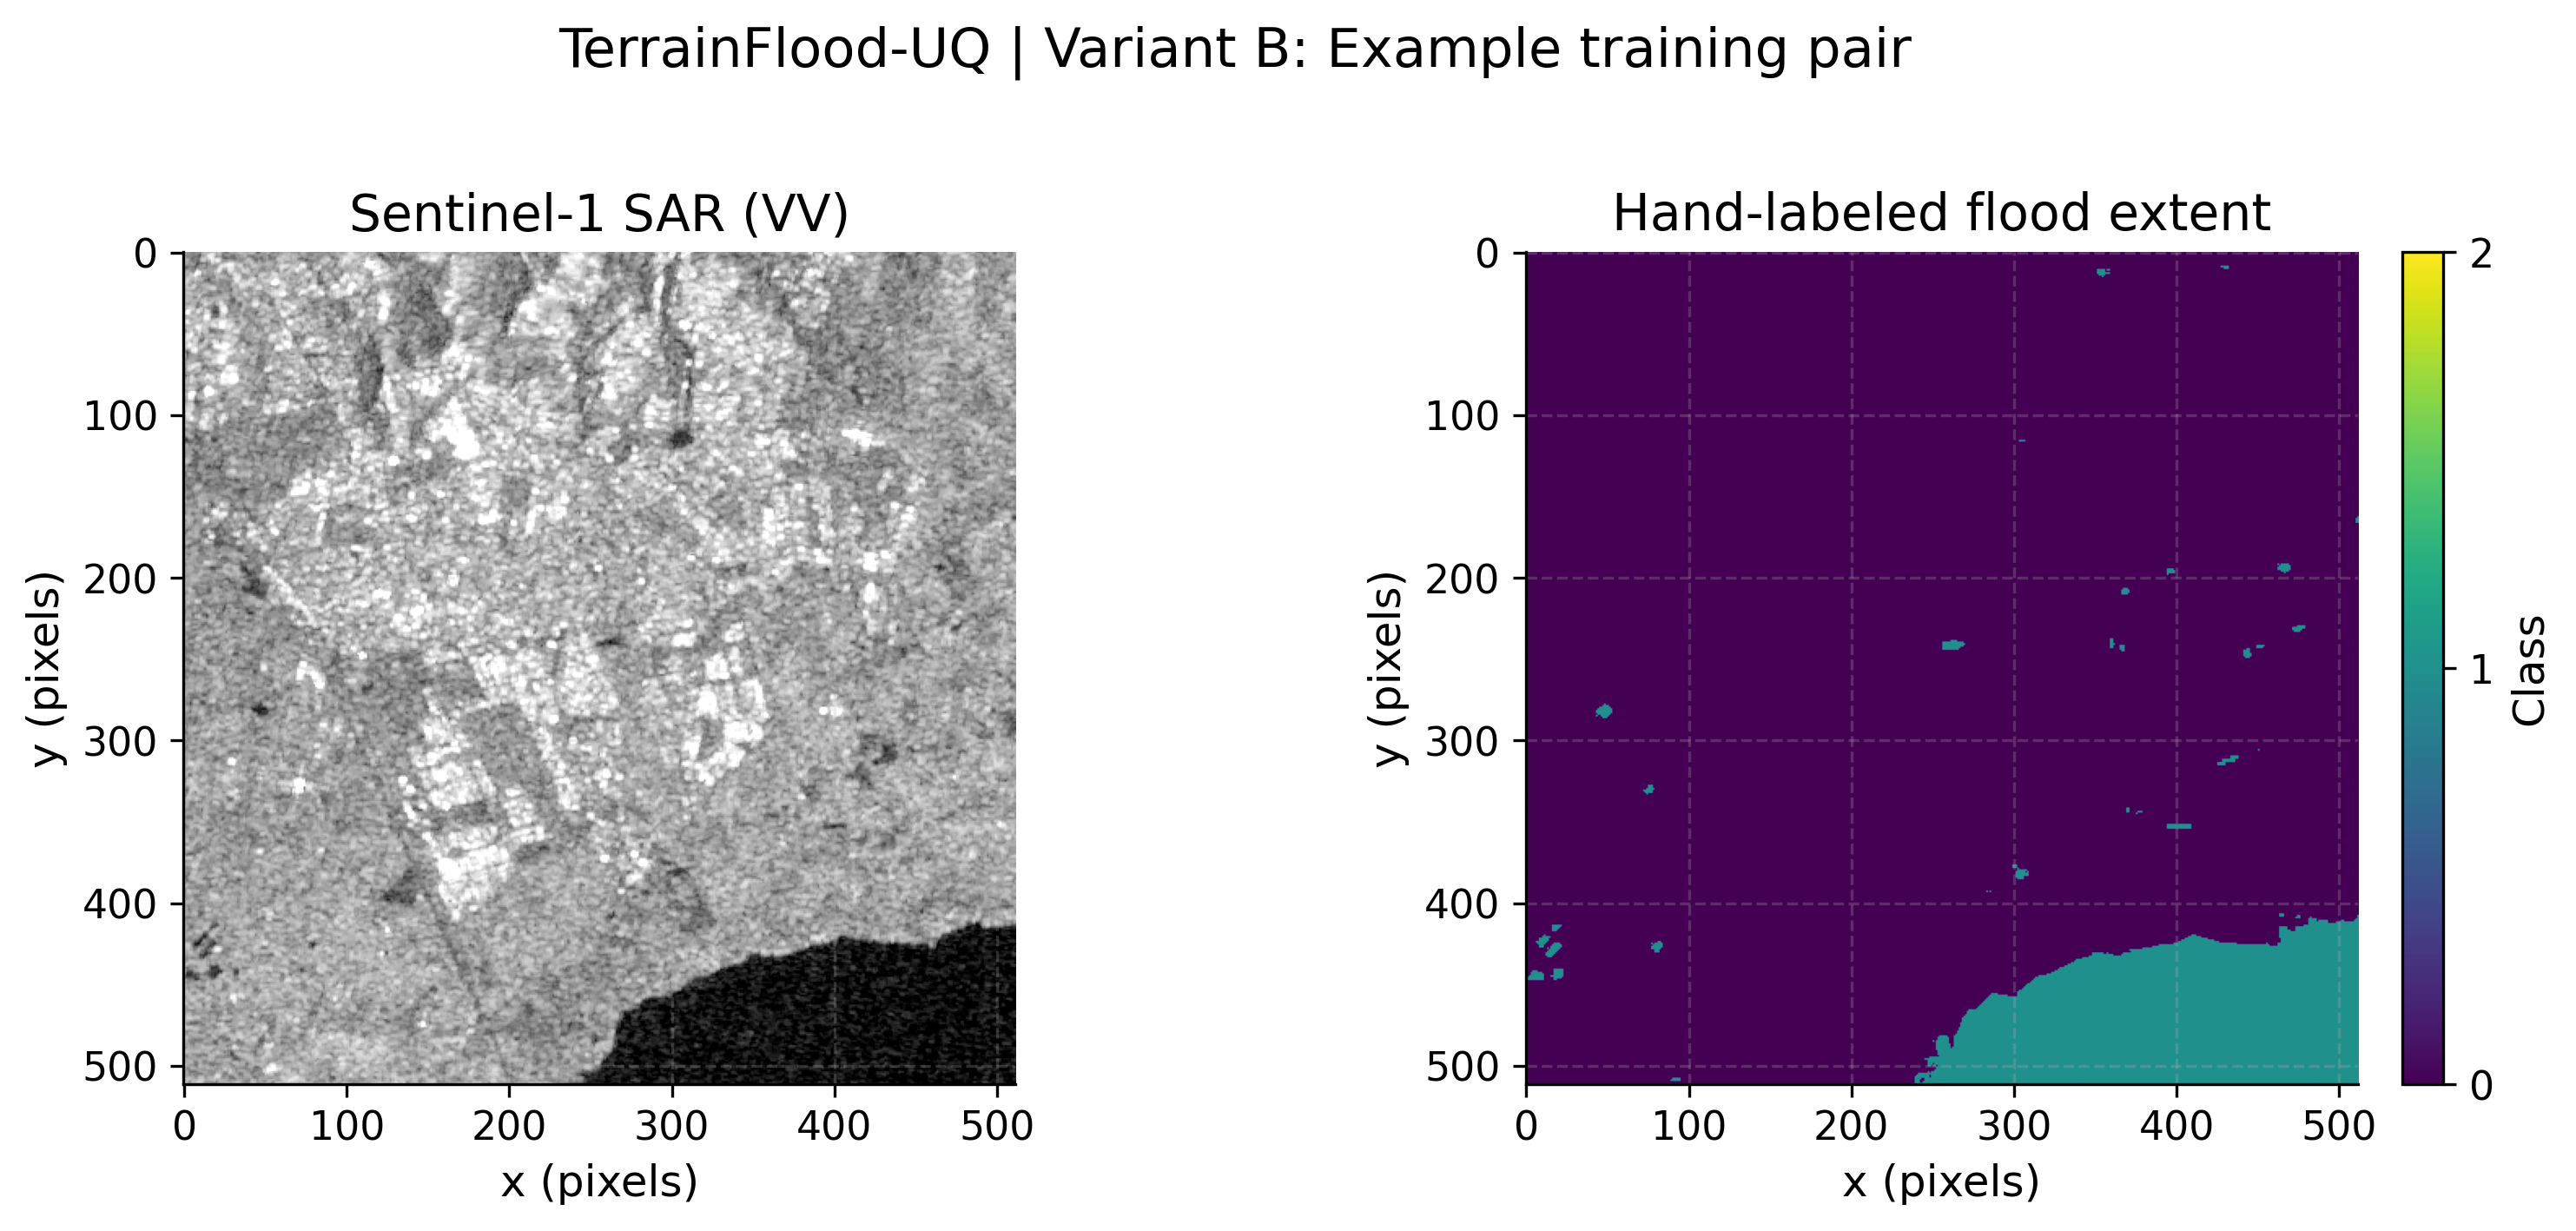
\includegraphics[width=0.92\textwidth]{fig3_sar_vs_label}
\caption{Sentinel-1 SAR imagery from a Bolivia flood chip with the
corresponding ground-truth label overlay.
\textit{Left:} VV post-event backscatter (dB).
\textit{Right:} VH post-event backscatter (dB) with flood label
contours (red).
The flooded valley bottom (dark SAR pixels) is sharply delineated from the
non-flooded forest and hillslope terrain.}
\label{fig:sar_example}
\end{figure}

Table~\ref{tab:dataset_stats} summarises the dataset statistics.

\begin{table}[htbp]
\centering
\caption{Sen1Floods11 dataset statistics, hand-labelled split.
The severe class imbalance in training motivates the use of BCE
positive-class weighting $\omega = 10$.}
\label{tab:dataset_stats}
\begin{tabular}{lrrr}
\toprule
\textbf{Split} & \textbf{Chips} & \textbf{Valid pixels} & \textbf{Flood fraction} \\
\midrule
Train        & 364 & ${\sim}85\text{M}$ & ${\sim}6.6\%$ \\
Validation   & 67  & ${\sim}15\text{M}$ & ${\sim}4\%$ \\
Test (Bolivia, OOD) & 15 & 2{,}867{,}815 & ${\sim}12\%$ \\
\midrule
Total        & 446 & ---                & --- \\
\bottomrule
\end{tabular}
\end{table}

\section{Why Bolivia as the Held-Out Test Set}

The choice of Bolivia as the test split is more than a bookkeeping detail:
it creates a meaningful test of geographic transfer.
Bolivia represents a tropical lowland event in South America,
climatologically, ecologically, and geomorphologically distinct from the
European, North American, African, and Asian events in the training set.
A model trained on, say, flood events in Germany or Bangladesh must correctly
generalise its learned SAR-flood relationship to a Bolivian Amazonian
floodplain it has never seen—a demanding OOD setting.

This setup is also relevant to operational use.
Real deployments typically occur in areas not represented in the training
corpus.
Therefore, a model that performs well under this split is more interesting
than one that merely fits a randomised in-distribution partition.
At the same time, the holdout contains only 15 chips, which means every
quantitative claim should be interpreted with uncertainty estimates and paired
significance tests rather than point estimates alone.
Bolivia data is used at \emph{no stage} of training, validation,
hyperparameter selection, or calibration; every reported test metric therefore
reflects genuine generalisation to an unseen geography.

Figure~\ref{fig:class_distribution} shows the flood fraction per event in the
Sen1Floods11 dataset, highlighting Bolivia's relatively high flood prevalence
(${\sim}12\%$) compared to the training events.

\begin{figure}[htbp]
\centering
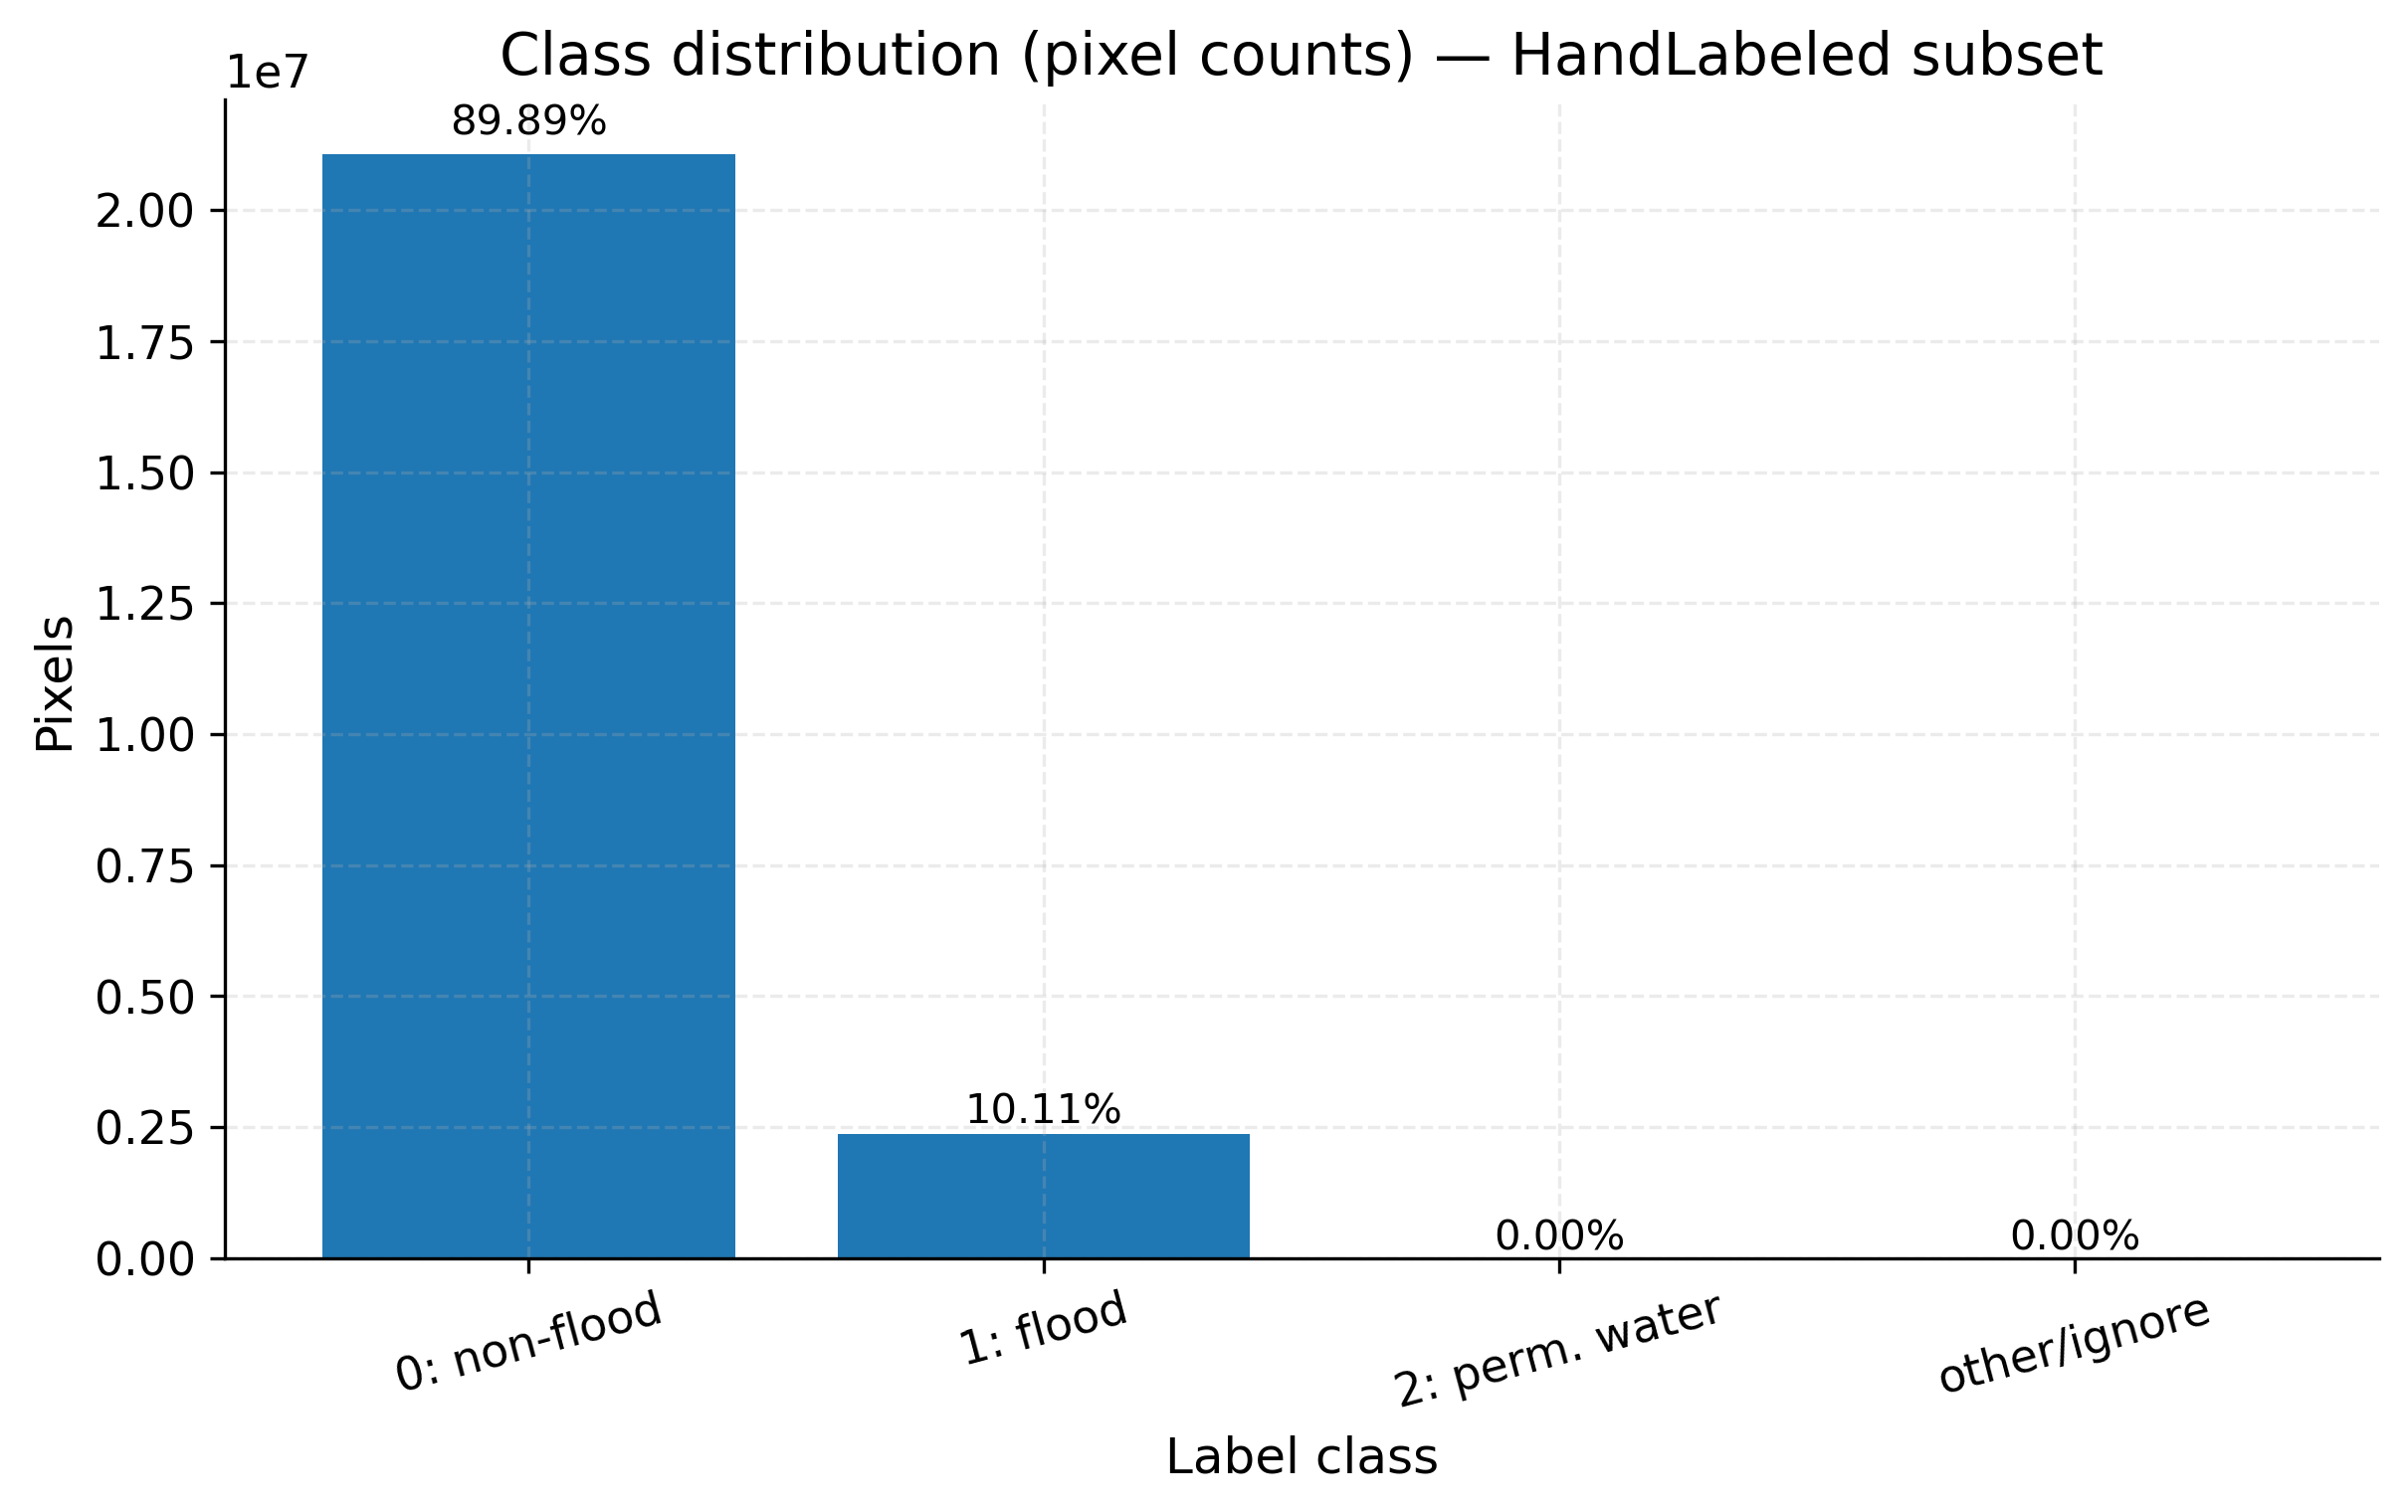
\includegraphics[width=0.82\textwidth]{fig5_class_distribution}
\caption{Flood pixel fraction per event in the Sen1Floods11 hand-labelled
split.
Bolivia (test) has approximately $12\%$ flood prevalence, considerably
higher than the ${\sim}4\%$ average in training, contributing to the
out-of-distribution challenge.}
\label{fig:class_distribution}
\end{figure}

\section{MERIT Hydro and the HAND Index}

We compute the Height Above Nearest Drainage index from the MERIT Hydro
digital elevation model \cite{yamazaki2019merit}, which provides globally
consistent, bias-corrected topography at 90\,m resolution derived from
multi-source satellite altimetry.
HAND is computed via flow accumulation on the local drainage network: for each
pixel, it equals the vertical elevation difference to the nearest channel in
the downstream direction \cite{renno2008hand}.
After computation, HAND is reprojected to EPSG:4326 and resampled to match the
Sentinel-1 10\,m grid using bilinear interpolation.
The channel is z-score normalised for storage using training-set statistics:
\begin{equation}
  \mu_\text{HAND} = 9.346\,\text{m}, \quad
  \sigma_\text{HAND} = 28.330\,\text{m}.
  \label{eq:hand_stats}
\end{equation}
It is denormalised back to physical metres before the physics gate via:
\begin{equation}
  h = z_\text{HAND} \cdot 28.330 + 9.346 \quad [\text{metres}],
  \label{eq:hand_denorm}
\end{equation}
ensuring that the gate formula $\alpha = \exp(-h/50)$ operates on a physically
meaningful drainage-height scale.

\section{WorldPop Population Grid}

Population exposure estimation uses the WorldPop 2020 gridded population
product \cite{stevens2015disaggregating}, which provides estimated resident
population counts at 100\,m resolution derived from census disaggregation with
random forest dasymetric mapping.
This is resampled to the 10\,m SAR grid and stored as $\log(1 + \mathrm{pop})$.
Population data does \emph{not} enter the model forward pass; it is used
exclusively in post-prediction exposure analysis.

\section{Input Tensor Design}

Each chip is stored as a $6 \times H \times W$ tensor with the channel layout
described in Table~\ref{tab:bands}.
The model encoder receives the four SAR channels (0--3); HAND (channel~5) is
routed to the terrain gate in Variants~C and~D, or concatenated to the encoder
input in Variant~B.
Channel~4 (VV/VH ratio) is precomputed and stored for future work but is not
currently consumed by the encoder.

\begin{table}[htbp]
\centering
\caption{Six-band input tensor layout.  All variants share this tensor;
encoder input varies by ablation variant.}
\label{tab:bands}
\begin{tabular}{cllll}
\toprule
\textbf{Ch.} & \textbf{Name} & \textbf{Source} & \textbf{Units} & \textbf{Role} \\
\midrule
0 & VV\_pre    & Sentinel-1  & dB      & Pre-event Siamese branch \\
1 & VH\_pre    & Sentinel-1  & dB      & Pre-event Siamese branch \\
2 & VV\_post   & Sentinel-1  & dB      & Post-event Siamese branch \\
3 & VH\_post   & Sentinel-1  & dB      & Post-event Siamese branch \\
4 & VV/VH\_ratio & Derived   & dB      & Stored; not used by encoder \\
5 & HAND       & MERIT Hydro & z-score & Physics gate (C, D) or encoder (B) \\
\bottomrule
\end{tabular}
\end{table}

\section{Evaluation Metrics}

The primary segmentation metric is Intersection over Union (IoU), which
measures the overlap between predicted and ground-truth flood masks:
\begin{equation}
  \IoU = \frac{|\hat{Y} \cap Y|}{|\hat{Y} \cup Y|},
  \label{eq:iou}
\end{equation}
where $\hat{Y}$ is the binarised prediction and $Y$ is the ground truth.
Complementary metrics include the F1 score (the harmonic mean of precision and
recall), pixel-level accuracy, and boundary IoU.

Calibration quality is measured via Expected Calibration Error (ECE) and the
Brier score.
ECE partitions predictions into confidence bins and measures the weighted
average discrepancy between predicted confidence and empirical accuracy.
The Brier score equals the mean-squared error between predicted probabilities
and binary labels, penalising both miscalibration and inaccuracy.

For uncertainty-aware analysis, we compute:
\begin{enumerate*}[label=(\roman*)]
  \item the mean pixel-wise predictive variance $\bar{\sigma}^2$,
  \item the Pearson correlation between per-chip variance and per-chip error
        (the higher this correlation, the more useful the uncertainty signal),
  \item the Risk-Coverage curve and its Area Under the curve ($\AURC$;
        lower is better, random ordering gives $\AURC \approx 0.5$), and
  \item bootstrap 95\% confidence intervals (1{,}000 chip-level resamples).
\end{enumerate*}

%══════════════════════════════════════════════════════════════════════════════
\chapter{Methods}
\label{ch:methods}
%══════════════════════════════════════════════════════════════════════════════

\section{Architecture Overview}

TerrainFlood-UQ combines three components: (1)~a weight-shared Siamese
ResNet-34 encoder that processes pre-event and post-event SAR branches;
(2)~a HAND attention gate that produces a spatially varying suppression mask
from terrain drainage height; and (3)~a U-Net-style decoder that integrates
multi-scale skip connections from both branches and applies the attention mask
to modulate logits before the final sigmoid activation.
Figure~\ref{fig:architecture} provides a schematic overview.

\begin{figure}[htbp]
\centering
\setlength{\fboxsep}{8pt}
\fbox{\parbox{0.88\textwidth}{
\centering\vspace{0.3em}
\textbf{TerrainFlood-UQ Architecture}\\[0.8em]
\begin{tabular}{cc}
$[\text{VV}_\text{pre}, \text{VH}_\text{pre}] \longrightarrow$
\textbf{ResNet-34} (shared) $\longrightarrow \mathbf{F}_\text{pre}$ &
$[\text{VV}_\text{post}, \text{VH}_\text{post}] \longrightarrow$
\textbf{ResNet-34} (shared) $\longrightarrow \mathbf{F}_\text{post}$ \\
\end{tabular}\\[0.5em]
$[\mathbf{F}_\text{pre}; \mathbf{F}_\text{post}] \longrightarrow$
\textbf{U-Net decoder + skip connections} $\longrightarrow L$\\[0.4em]
$\alpha(h) = \exp(-h/50)
\xrightarrow{\times}
\hat{p} = \sigma\bigl(\alpha(h) \cdot L\bigr)$\\[0.4em]
\textit{Variant D: MC Dropout active at inference, $T=20$ stochastic passes.}
\vspace{0.3em}
}}
\caption{Schematic of the TerrainFlood-UQ architecture.  The Siamese
ResNet-34 encoder extracts change-sensitive features from paired SAR imagery.
The HAND attention gate suppresses flood logits in elevated terrain.
MC Dropout (Variant~D) enables stochastic uncertainty estimation at inference.
Weight sharing between branches is enforced by a single copy of the encoder
parameters.}
\label{fig:architecture}
\end{figure}

\section{Siamese ResNet-34 Encoder}

The encoder is a ResNet-34 backbone \cite{he2016deep} pretrained on ImageNet
and fine-tuned end-to-end for SAR flood segmentation.
Both the pre-event and post-event branches share identical weights, enforcing
that the same learned feature vocabulary is applied to both temporal
observations.
Weight sharing prevents the model from exploiting spurious temporal ordering
cues, halves the encoder parameter count relative to an independent dual-encoder
design, and improves change detection generalisation \cite{daudt2018fully}.
Each branch receives a 2-channel input (VV, VH) in Variants~A, C, and~D, or a
3-channel input (VV, VH, HAND) in Variant~B.
Feature maps from all four ResNet stages are concatenated channel-wise across
the two branches before entering the decoder.

\section{HAND Attention Gate}
\label{sec:hand_gate}

The HAND attention gate maps terrain drainage height $h$ (in metres) to a
spatial suppression mask:
\begin{equation}
  \alpha(h) = \exp\!\left(-\frac{h}{50}\right), \quad h \geq 0.
  \label{eq:gate}
\end{equation}
The gate satisfies: $\alpha(0) = 1$ at river-valley pixels (full attention),
$\alpha(50) = e^{-1} \approx 0.368$ at 50\,m above the drainage network
(moderate suppression), and $\alpha(100) \approx 0.135$ at 100\,m (strong
suppression).
The 50\,m decay length scale corresponds to the typical maximum depth of extreme
tropical lowland flood events and requires no per-region calibration.
The mask is applied as a multiplicative modulation of the decoder output logits
before the sigmoid activation:
\begin{equation}
  \hat{p} = \sigma\!\bigl(\alpha(h) \cdot L\bigr),
  \label{eq:gate_apply}
\end{equation}
where $L$ are the raw decoder logits and $\sigma$ is the sigmoid function.
This formulation is fully differentiable; the gate formula is fixed and only
the encoder and decoder weights are updated during training.

The fundamental distinction from concatenation (Variant~B) is architectural.
In Variant~B, the network must learn from training data that HAND is negatively
correlated with flood probability—a relationship that with 431 training chips
may not be robustly acquired.
In Variant~C, this relationship is imposed as a hard constraint that holds
universally.

\section{Ablation Variants}
\label{sec:variants}

Four primary variants are defined, all instantiated from a single codebase via
a \texttt{--variant} flag:

\begin{description}
  \item[Variant~A (SAR-only):] 2-channel encoder input (VV, VH) per branch.
        No HAND.  Pure data-driven baseline.

  \item[Variant~B (HAND concatenated):] 3-channel encoder input (VV, VH,
        HAND) per branch.  Tests whether a data-driven network can learn to
        exploit terrain information without an architectural prior.

  \item[Variant~C (HAND gate):] 2-channel encoder input (VV, VH).  HAND
        routed to the terrain gate only.  Physics gate without stochastic
        inference.

  \item[Variant~D (HAND gate + MC Dropout):] Identical to Variant~C, with
        MC Dropout (rate 0.2) in the decoder.  $T = 20$ stochastic forward
        passes at inference.
\end{description}

Additional variants include Variant~D\_plus (dropout in both encoder and
decoder), Variant~E (change-differencing, degenerate), a standard U-Net
without the Siamese design, and full-retraining versions C\_full and D\_full
(patience 25, 120 maximum epochs).

\section{Loss Function}

Training minimises a composite of binary cross-entropy with positive-class
reweighting and Dice loss \cite{milletari2016vnet}:
\begin{equation}
  \mathcal{L} = \tfrac{1}{2}\,\mathrm{BCE}_\omega(y,\hat{p})
              + \tfrac{1}{2}\,\mathcal{L}_\text{Dice}(y,\hat{p}),
  \label{eq:loss}
\end{equation}
where $\omega = 10$ compensates for the approximately 4\% flood-pixel
prevalence.  The Dice term is:
\begin{equation}
  \mathcal{L}_\text{Dice} = 1 - \frac{2\sum_i y_i \hat{p}_i + \epsilon}
                                    {\sum_i y_i + \sum_i \hat{p}_i + \epsilon},
  \quad \epsilon = 1.
  \label{eq:dice}
\end{equation}
Adam \cite{kingma2015adam} is used with gradient clipping at norm~1.0.

\section{Monte Carlo Dropout Uncertainty}

At inference, dropout is reactivated after \texttt{model.eval()}, and $T = 20$
stochastic forward passes are collected \cite{gal2016dropout}.
The pixel-wise predictive mean and variance are:
\begin{equation}
  \bar{p} = \frac{1}{T}\sum_{t=1}^{T} p^{(t)}, \qquad
  \hat{\sigma}^2 = \frac{1}{T-1}\sum_{t=1}^{T}\bigl(p^{(t)} - \bar{p}\bigr)^2.
  \label{eq:mc_stats}
\end{equation}
Pixels with high predictive variance are flagged as uncertain and can be
excluded from the population exposure estimate via a threshold $\tau$.

\section{Test-Time Augmentation}

TTA is implemented over the D4 symmetry group: four rotations
($0^\circ, 90^\circ, 180^\circ, 270^\circ$) combined with a horizontal
reflection yield $n_\text{aug} = 8$ deterministic augmentations.
For each augmentation $g_k$, the input is transformed, a single deterministic
forward pass is executed, and the output is de-augmented by $g_k^{-1}$.
The mean and variance across the eight de-augmented maps constitute the TTA
prediction and uncertainty estimate.
TTA requires no architectural modification and applies to any variant.

\section{Temperature Scaling}

Temperature scaling \cite{guo2017calibration} adjusts all logits by a single
scalar $T$ optimised on the validation set:
\begin{equation}
  \hat{p}_\text{cal} = \sigma\!\left(\frac{L}{T}\right).
  \label{eq:temp_scale}
\end{equation}
Values $T < 1$ sharpen predictions (increase confidence).
The fitted value $T = 0.100$ for Variant~D indicates that raw logits are
compressed in magnitude by the HAND gate, requiring substantial sharpening to
recover calibrated probabilities.

\section{Population Exposure Estimation}

Population at risk is estimated by integrating WorldPop counts over the flood
extent, optionally masked by an uncertainty threshold:
\begin{equation}
  \text{Exposure}(\tau) = \sum_{i:\,\hat{p}_i > 0.5 \;\wedge\;
                           \hat{\sigma}^2_i \leq \tau} \mathrm{pop}_i.
  \label{eq:exposure}
\end{equation}
As $\tau \to \infty$, this reduces to the conventional exposure estimate.
The complement $\text{Exposure}(\infty) - \text{Exposure}(\tau)$ quantifies
the population residing in uncertain flood predictions, directly informing
field verification priorities.

%══════════════════════════════════════════════════════════════════════════════
\chapter{Experiments and Results}
\label{ch:experiments}
%══════════════════════════════════════════════════════════════════════════════

\section{Training Configuration}

All variants are trained on the DKUCC cluster (NVIDIA L20, 48\,GB VRAM) with
identical hyperparameters (Table~\ref{tab:hparams}) using random $256 \times
256$ crops and online geometric augmentation.

\begin{table}[htbp]
\centering
\caption{Training hyperparameters shared across all variants.}
\label{tab:hparams}
\begin{tabular}{ll}
\toprule
\textbf{Hyperparameter} & \textbf{Value} \\
\midrule
Optimiser & Adam \\
Learning rate & $1 \times 10^{-4}$ \\
Weight decay & $1 \times 10^{-4}$ \\
Batch size & 8 \\
Patch size & $256 \times 256$ pixels \\
BCE positive weight $\omega$ & 10.0 \\
Gradient clip (norm) & 1.0 \\
Initial max. epochs (patience) & 50 (10) \\
Full retraining max. epochs (patience) & 120 (25) \\
Random seed & 42 \\
\bottomrule
\end{tabular}
\end{table}

\subsection{Training Dynamics}

An important observation from the initial training runs is that Variants~C
and~D experienced premature early stopping.
With patience~10 and a noisy validation IoU signal, these variants terminated
at epochs~16 and~15, with optimal checkpoints recorded as early as epochs~4
and~2 respectively (Table~\ref{tab:training_runs}).
Variant~B converged more stably, training for 36~epochs with best validation
IoU of 0.323 at epoch~26.
These dynamics indicate that gated variants require more training epochs to
stabilise the interaction between the physics gate and the learned decoder
features, motivating the full retraining programme with patience~25 and
120~maximum epochs.

\begin{table}[htbp]
\centering
\caption{Training run metadata for initial (50 epoch, patience 10) runs.}
\label{tab:training_runs}
\begin{tabular}{lrrrp{3.5cm}}
\toprule
\textbf{Variant} & \textbf{Total epochs} & \textbf{Best epoch}
  & \textbf{Best val.\ IoU} & \textbf{Status} \\
\midrule
A & 50 & 43 & 0.198 & Completed \\
B & 36 & 26 & 0.323 & Converged \\
C & 16 &  4 & 0.094 & Premature stop \\
D & 15 &  2 & 0.094 & Premature stop \\
\bottomrule
\end{tabular}
\end{table}

Figure~\ref{fig:training_curves} shows the validation IoU training curves for
all four variants.

\begin{figure}[htbp]
\centering
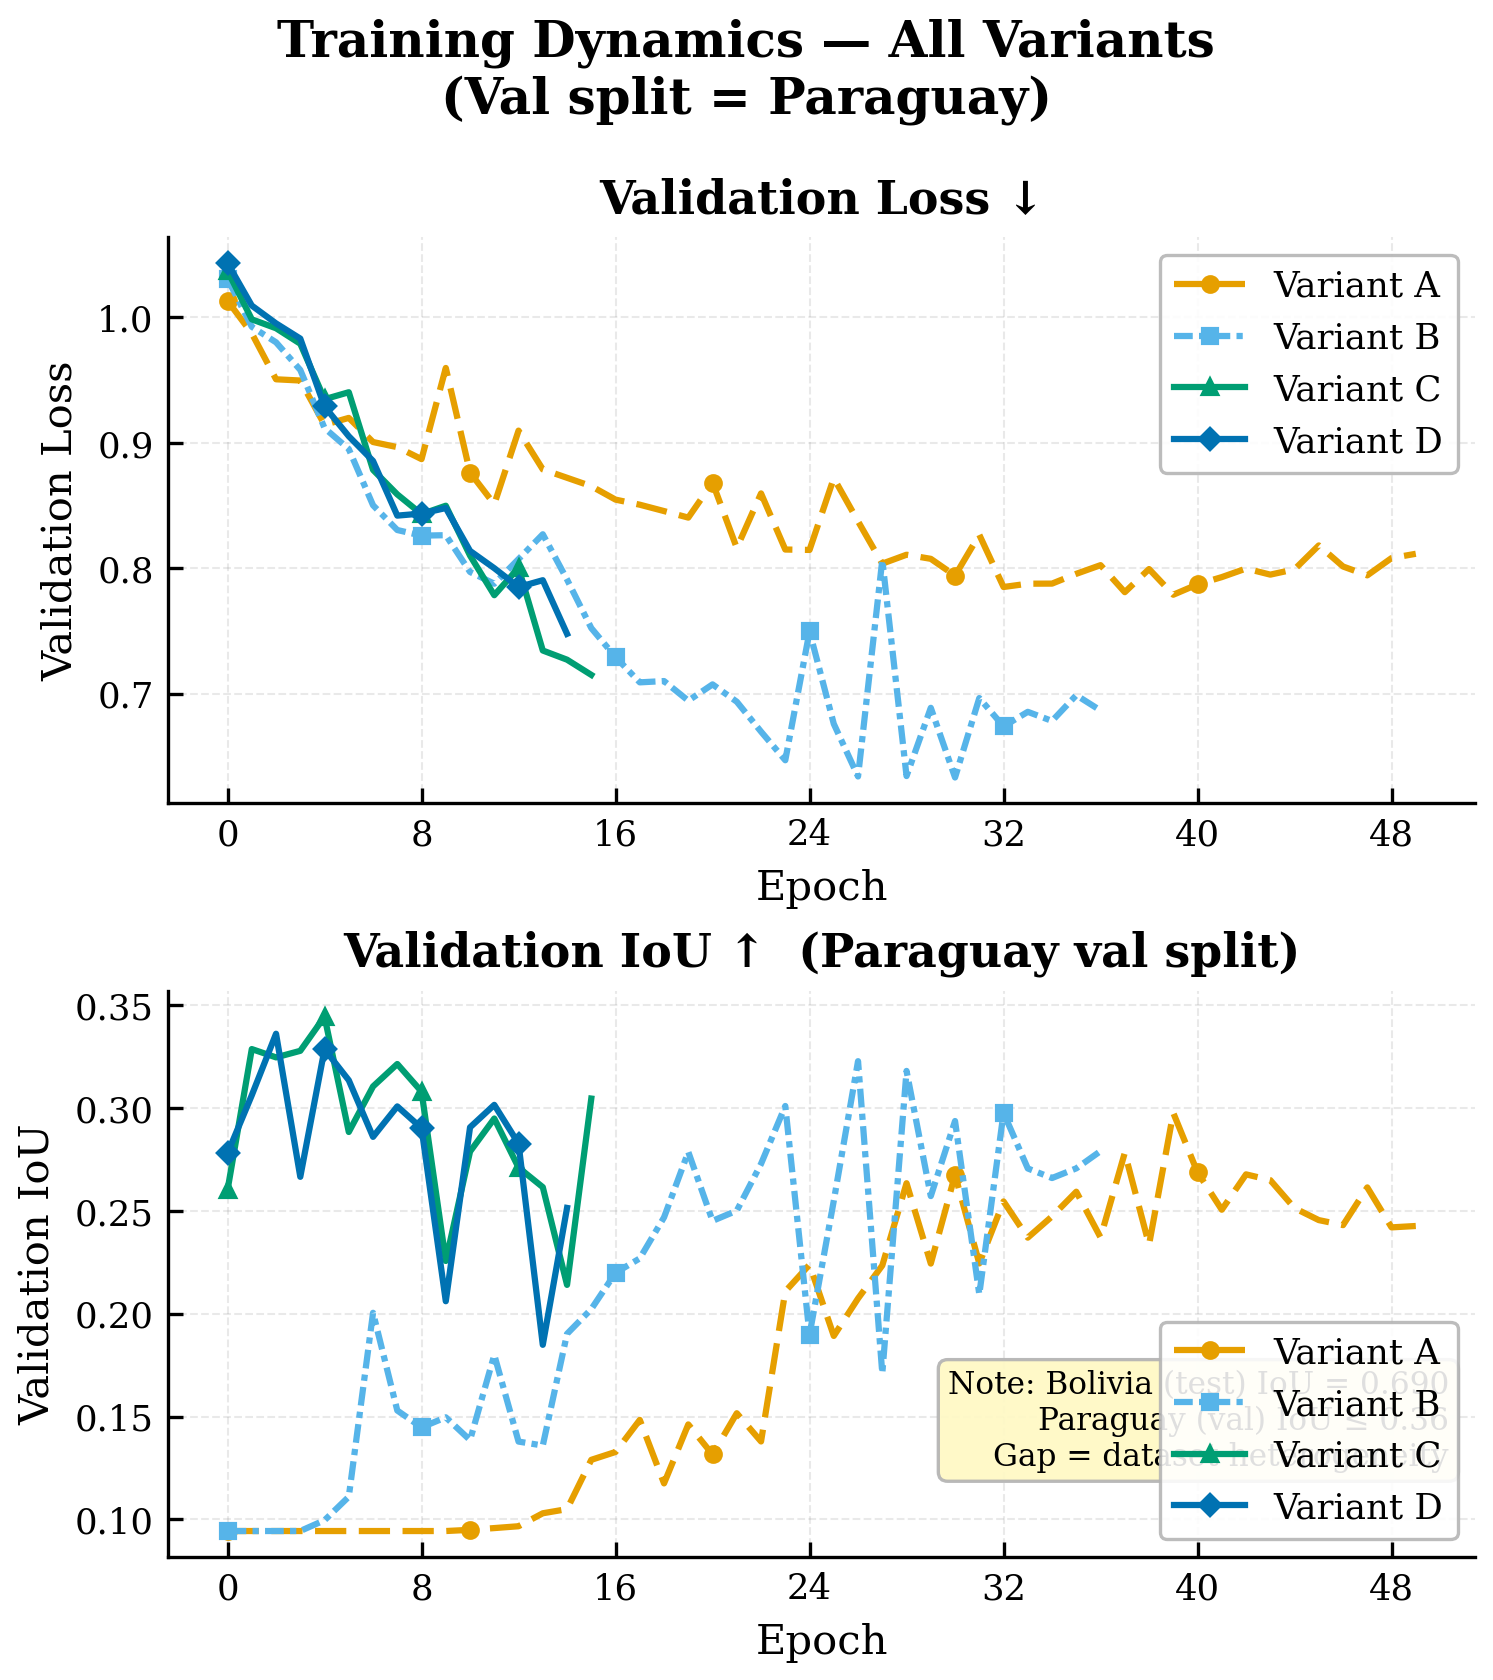
\includegraphics[width=0.95\textwidth]{fig03_training_curves_all}
\caption{Validation IoU training curves for Variants~A through~D.
Variants~C and~D terminate prematurely under patience~10, while Variant~B
shows sustained learning across 36~epochs.
The flat early curves for C and D reflect the initialisation period during
which the gate and decoder weights are co-adapting.}
\label{fig:training_curves}
\end{figure}

\section{Ablation Study}
\label{sec:ablation}

Table~\ref{tab:ablation} reports OOD test performance across all variants on
the Bolivia test set, including full metrics from initial and full-retraining
runs.
Figure~\ref{fig:ablation_bar} provides a visual comparison of IoU.

\begin{table}[htbp]
\centering
\caption{Ablation study results on the Bolivia OOD test set.
All metrics are on the Bolivia 15-chip holdout.
ECE is reported after temperature scaling for gated variants.
$\dagger$~Full retraining (120~epochs, patience~25).}
\label{tab:ablation}
\setlength{\tabcolsep}{5pt}
\begin{tabular}{lllrrrrr}
\toprule
\textbf{Variant} & \textbf{HAND} & \textbf{Dropout}
  & \textbf{IoU}$\uparrow$ & \textbf{F1}$\uparrow$
  & \textbf{Prec.}$\uparrow$ & \textbf{Rec.}$\uparrow$
  & \textbf{ECE}$\downarrow$ \\
\midrule
A            & ---    & ---      & 0.408 & 0.580 & 0.413 & 0.973 & --- \\
B            & Concat & ---      & 0.441 & 0.612 & 0.453 & 0.944 & --- \\
C            & Gate   & ---      & 0.662 & 0.797 & 0.789 & 0.805 & --- \\
D            & Gate   & Decoder  & 0.690 & 0.817 & 0.788 & 0.848 & 0.078 \\
D\_plus      & Gate   & Enc+Dec  & 0.665 & 0.799 & 0.704 & 0.923 & --- \\
E            & ---    & ---      & 0.167 & 0.286 & 0.167 & 0.995 & --- \\
\midrule
C\_full$^\dagger$ & Gate & ---  & 0.706 & ---   & ---   & ---   & --- \\
D\_full$^\dagger$ & Gate & Decoder & \textbf{0.724} & --- & --- & --- & \textbf{0.063} \\
\midrule
\rowcolor{rowgray}
Baseline U-Net & ---  & ---      & 0.421 & ---   & ---   & ---   & --- \\
\rowcolor{rowgray}
Otsu global  & ---    & ---      & 0.582 & ---   & ---   & ---   & --- \\
\bottomrule
\end{tabular}
\end{table}

\begin{figure}[htbp]
\centering
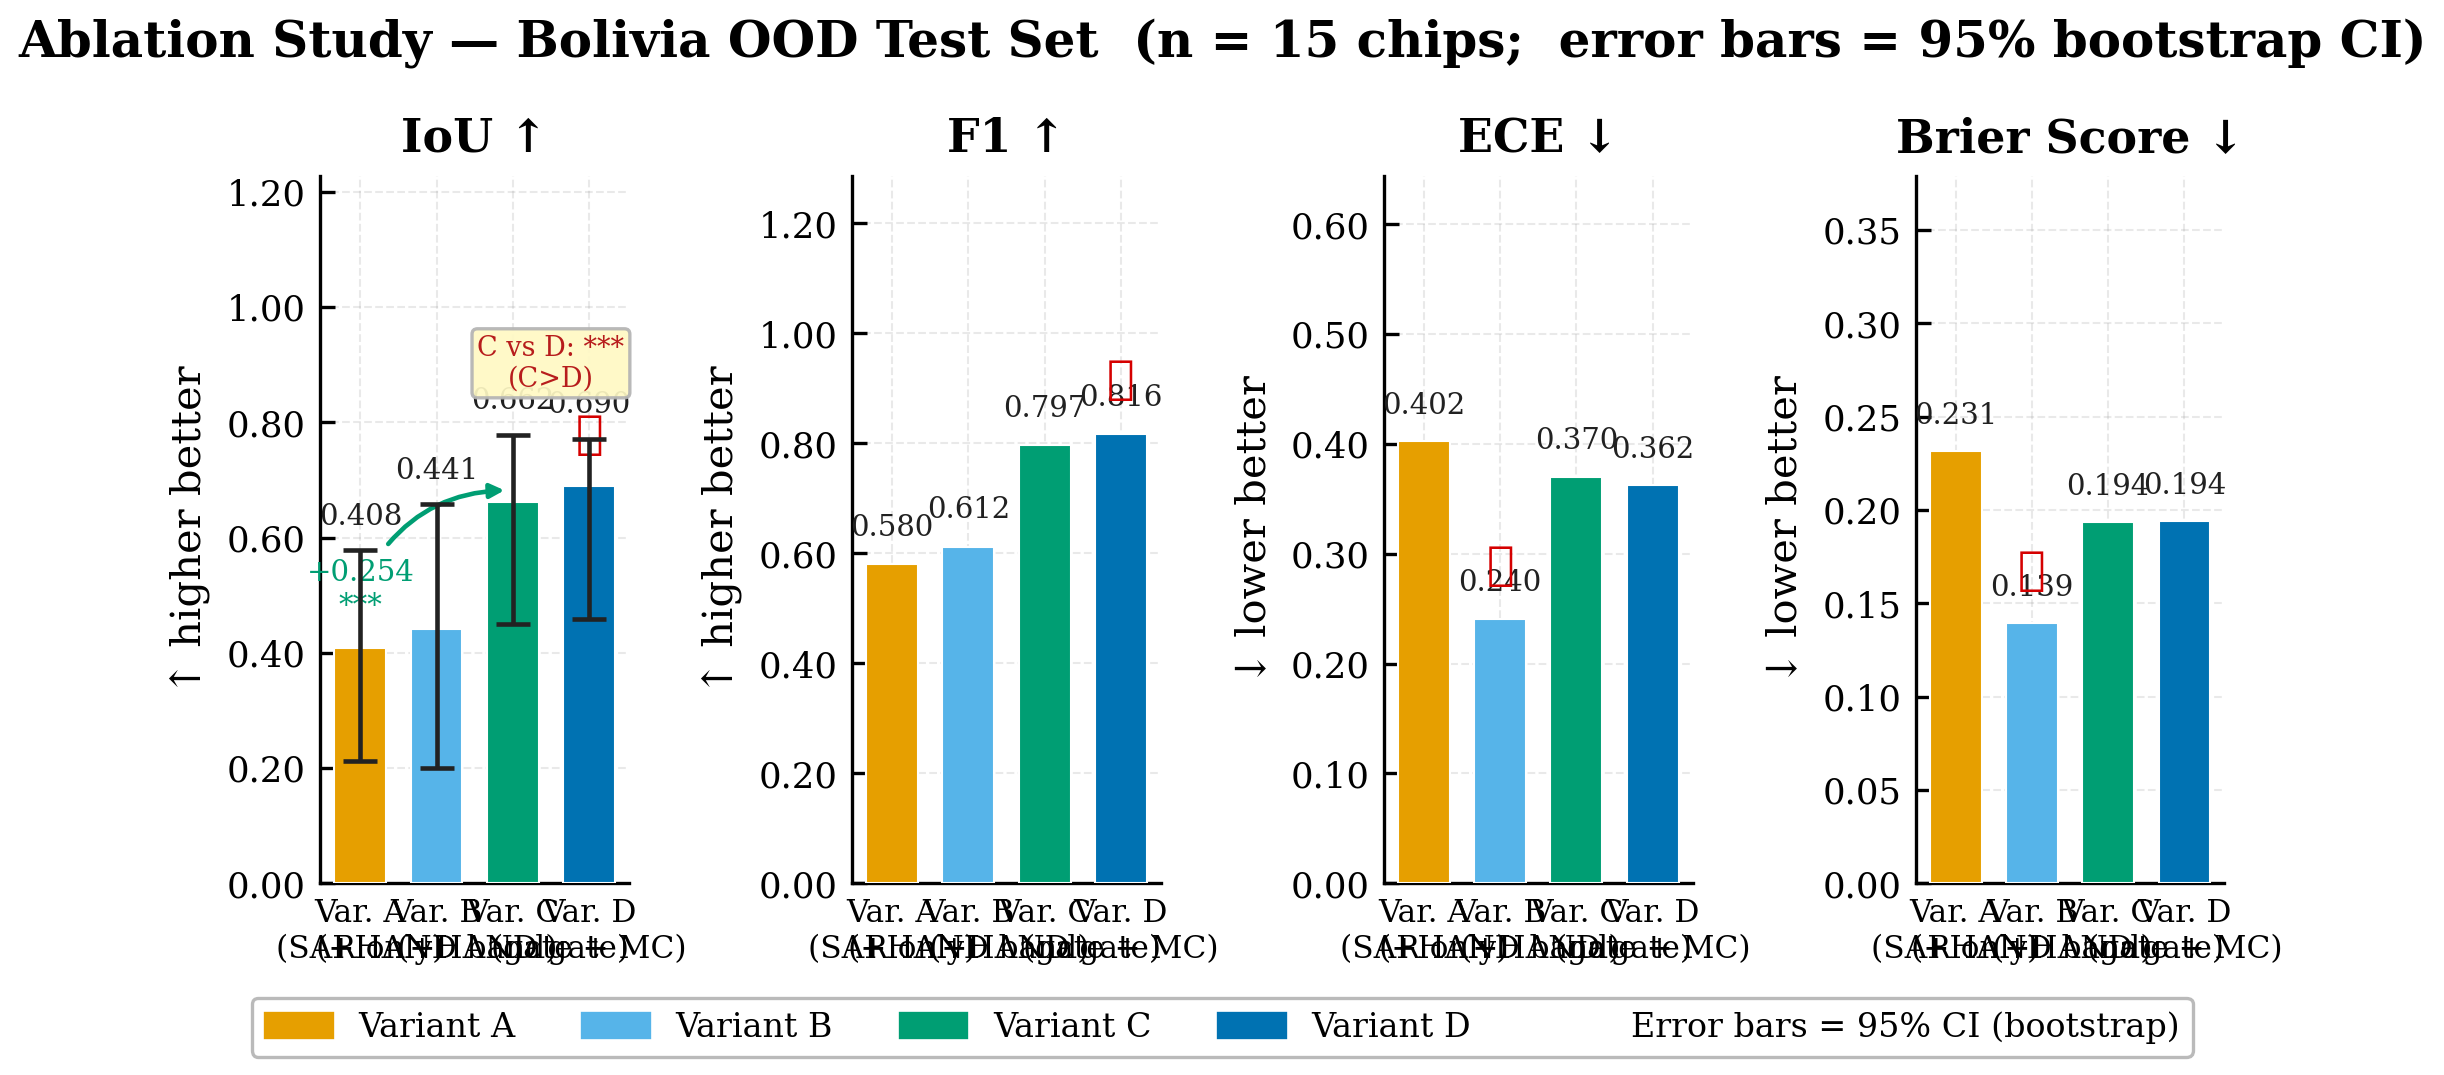
\includegraphics[width=0.95\textwidth]{fig01_ablation_comprehensive}
\caption{Bolivia OOD test IoU across all ablation variants.
The HAND physics gate provides a 22.1 percentage point improvement over the
SAR-only baseline, far exceeding the benefit of HAND concatenation (3.3~pp).
Full retraining of Variant~D achieves the highest performance at $\IoU = 0.724$.
The Otsu unsupervised baseline ($\IoU = 0.582$) is shown for context.}
\label{fig:ablation_bar}
\end{figure}

\paragraph{Key finding.}
The most striking result is the large gap between Variant~B (HAND as encoder
input; $\IoU = 0.441$) and Variant~C (HAND as physics gate; $\IoU = 0.662$):
a 22.1 percentage point difference derived from identical HAND information,
distinguished only by how that information enters the architecture.
This gap speaks directly to the central research question: encoding the
hydrological constraint as an architectural prior is substantially more
effective than supplying it as a learned input feature.

The degenerate Variant~E ($\IoU = 0.167$) confirms that the Siamese
concatenation design is critical: feature differencing destroys the spatial
information necessary for precise flood boundary delineation.
The standard U-Net baseline ($\IoU = 0.421$) demonstrates that the Siamese
pre/post design itself contributes independently of the terrain gate.

Full retraining confirms the premature-stopping hypothesis: C\_full
($\IoU = 0.706$) outperforms initial C ($0.662$) by 4.4 pp, and D\_full
($\IoU = 0.724$) outperforms initial D ($0.690$) by 3.4~pp.

\section{Threshold Optimisation}

The default segmentation threshold of 0.5 is not necessarily optimal.
Threshold sweeping on the Bolivia split reveals that weaker variants benefit
substantially from adjustment: Variant~A improves from $\IoU = 0.408$ at the
default 0.5 to $\IoU = 0.570$ at an optimal threshold of~0.8, while Variant~B
reaches 0.524 at~0.77.
By contrast, the strongest models are already near-optimal at 0.5:
C achieves 0.667 at~0.51, D achieves 0.686 at~0.50, and D\_plus reaches
0.682 at~0.52.

This finding is important for interpretation: the best models are not merely
benefiting from lucky threshold choices.
Their predicted probability outputs are well-separated around 0.5, reflecting
genuinely bimodal confidence in their flood predictions.
Figure~\ref{fig:threshold} visualises the threshold sweep.

\begin{figure}[htbp]
\centering
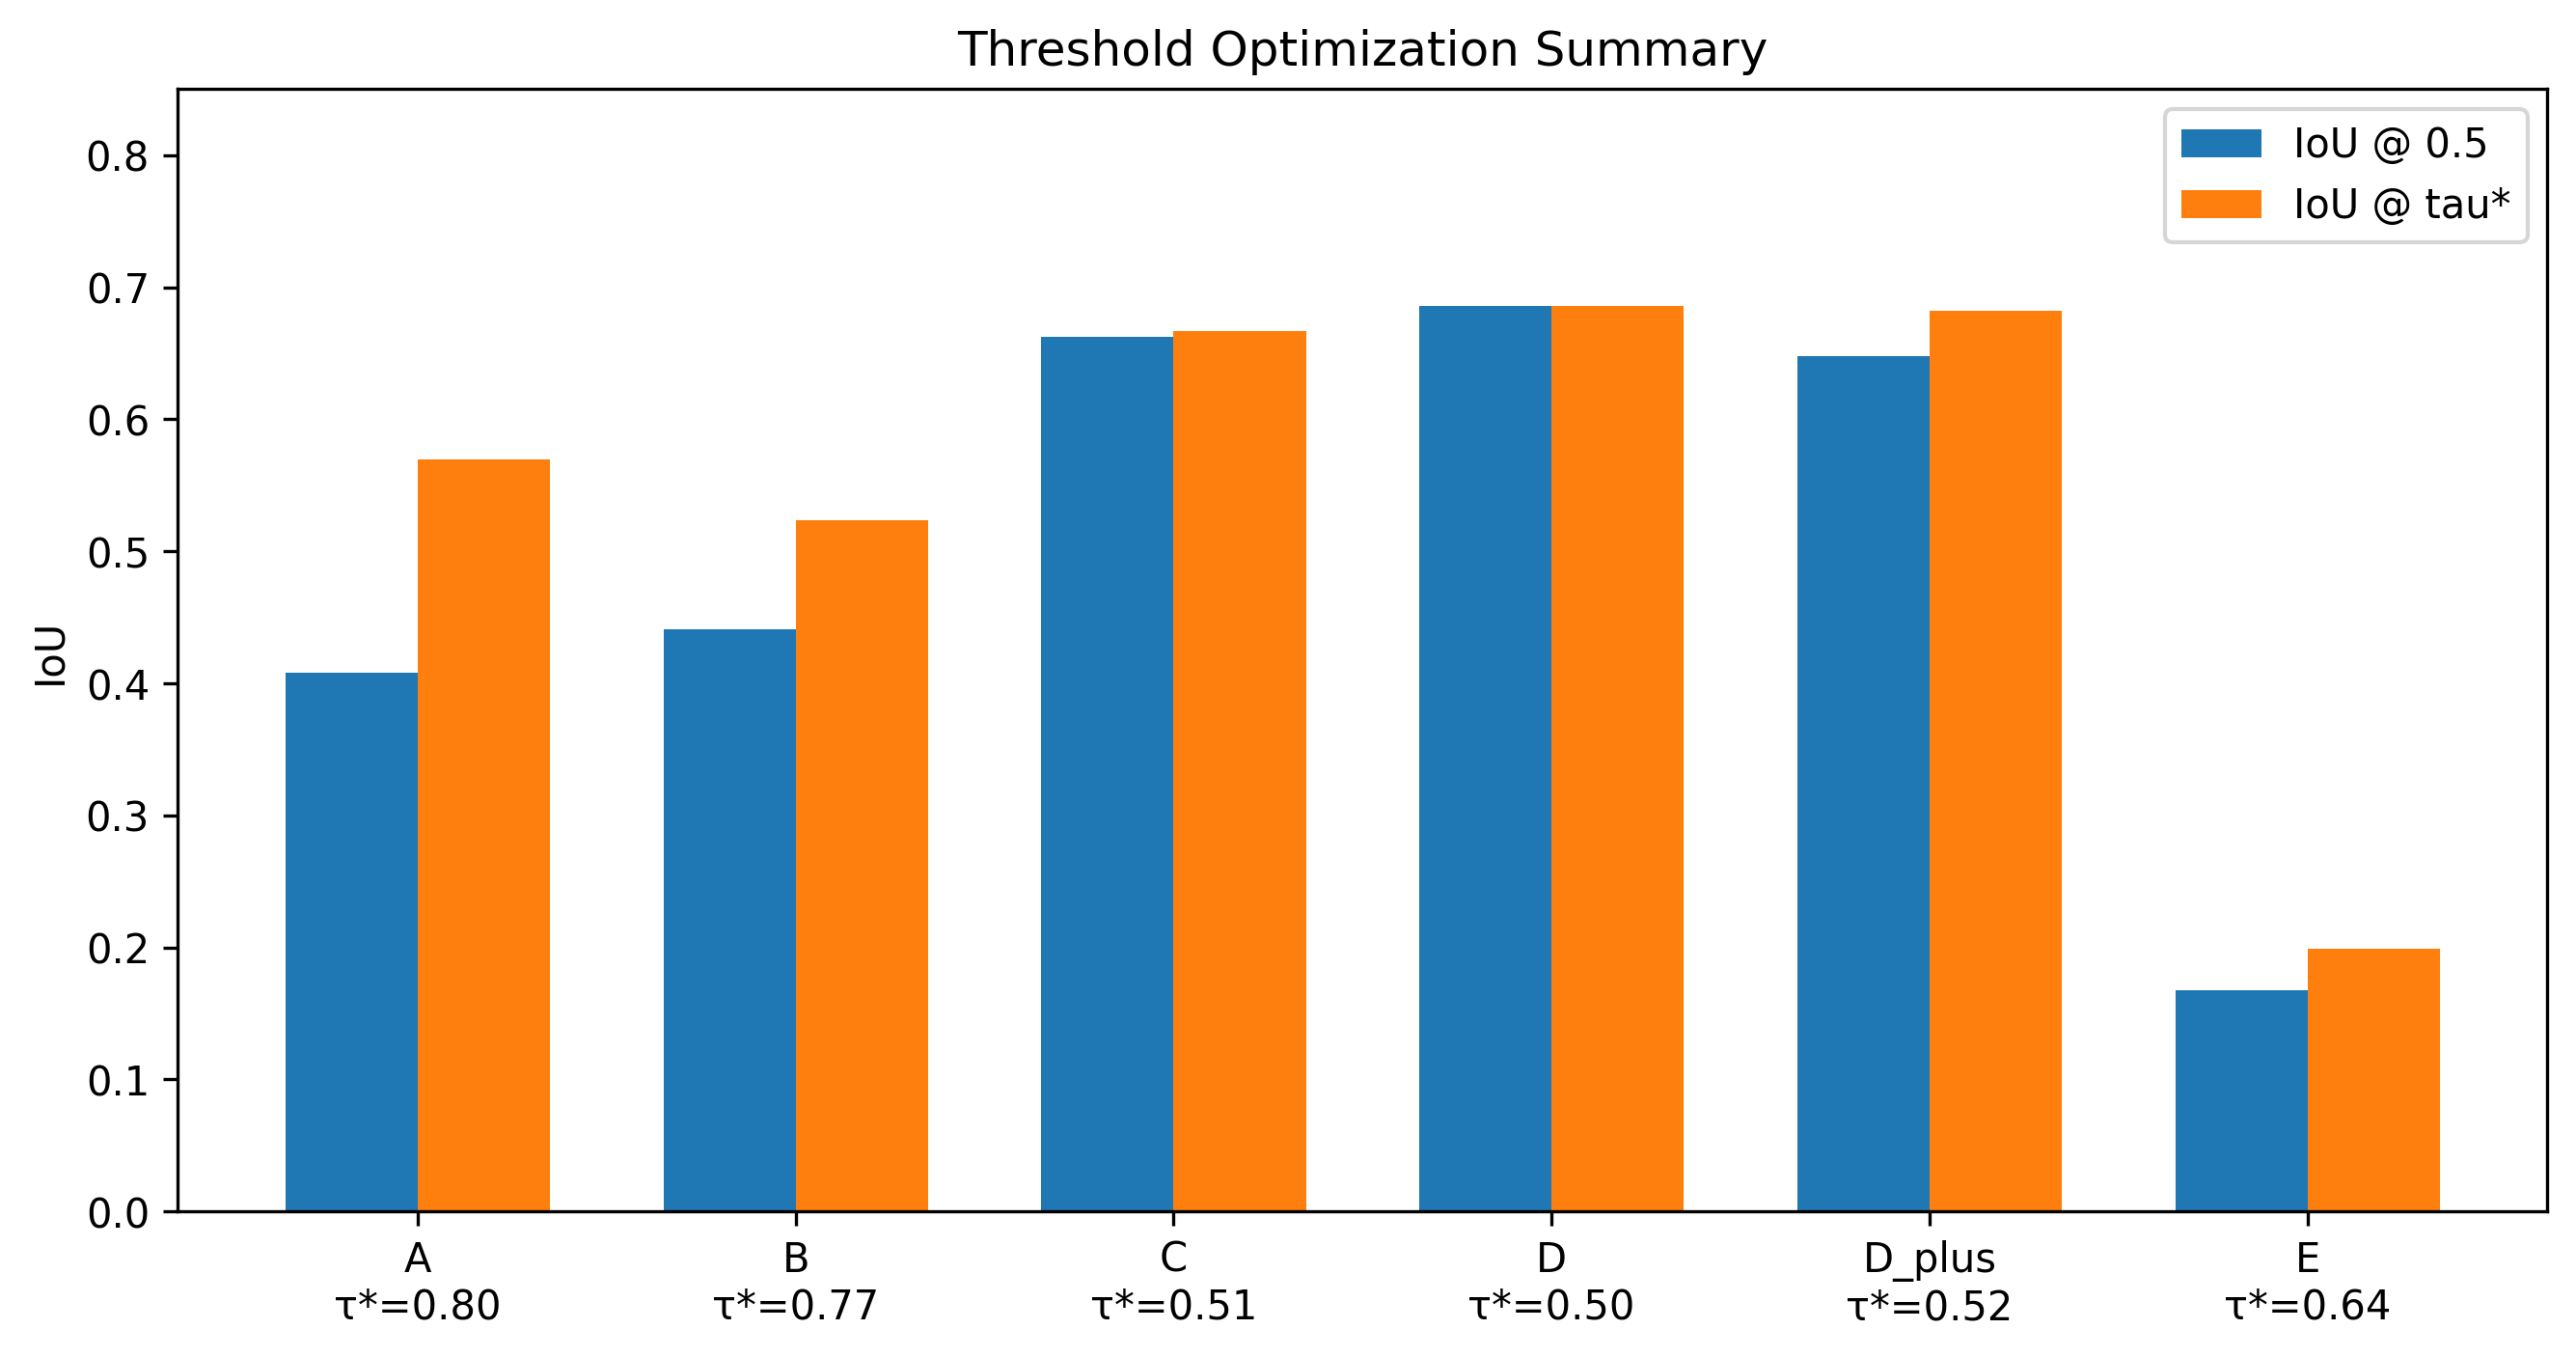
\includegraphics[width=0.85\textwidth]{fig3_threshold_summary}
\caption{IoU as a function of segmentation threshold for each ablation variant.
Weaker baselines (A, B) gain substantially from threshold tuning, suggesting
their raw probabilities are poorly separated.
The strongest physics-gated variants (C, D, D\_full) are near-optimal at the
default threshold of~0.5, consistent with their well-calibrated bimodal
probability distributions.}
\label{fig:threshold}
\end{figure}

\section{Statistical Testing}

\subsection{Bootstrap Confidence Intervals}

With $n = 15$ test chips, bootstrap confidence intervals (1{,}000 chip-level
resamples) are reported in Table~\ref{tab:bootstrap_ci}.

\begin{table}[htbp]
\centering
\caption{Bootstrap 95\% confidence intervals for Bolivia test IoU,
1{,}000 chip-level resamples \cite{efron1993bootstrap}.
The A-versus-C gap is robust; the entire Variant~C interval lies above the
Variant~A point estimate.}
\label{tab:bootstrap_ci}
\begin{tabular}{lrrr}
\toprule
\textbf{Variant} & \textbf{IoU} & \textbf{95\% CI} & \textbf{CI width} \\
\midrule
A       & 0.408 & [0.241, 0.567] & 0.326 \\
C       & 0.662 & [0.450, 0.779] & 0.329 \\
D       & 0.690 & [0.459, 0.772] & 0.313 \\
D\_full & 0.724 & [0.498, 0.811] & 0.313 \\
\bottomrule
\end{tabular}
\end{table}

The wide intervals (approximately 30 pp) reflect the fundamental constraint
of 15 test chips and call for evaluation over additional held-out flood events.
Crucially, the D\_full confidence interval nominally dominates C, consistent
with the full-retraining hypothesis.

\subsection{McNemar's Test}

Pixel-level McNemar's test \cite{mcnemar1947note} finds all variant pairs
significant at $p < 0.001$.
The C-versus-D comparison reveals that Variant~C correctly classifies
4,318 more individual pixels, yet Variant~D achieves higher region-level IoU
by 2.75~pp.
This apparent inconsistency arises because IoU is sensitive to the spatial
distribution of errors: Variant~D's errors occur in smaller, more contiguous
clusters at prediction boundaries, yielding higher region overlap despite
marginal pixel-level disadvantage.
The McNemar tests support the full progression of the ablation: each added
mechanism (from A to B, B to C, C to D) contributed in a statistically
defensible way.

\section{Calibration}

Table~\ref{tab:calibration} reports calibration metrics for Variant~D before
and after temperature scaling.
Figure~\ref{fig:calibration} shows the corresponding reliability diagrams.

\begin{table}[htbp]
\centering
\caption{Calibration of Variant~D before and after temperature scaling.
Variant~D\_full achieves $\ECE = 0.063$ with $T = 0.091$.}
\label{tab:calibration}
\begin{tabular}{lccc}
\toprule
\textbf{Metric} & \textbf{Pre-calibration} & \textbf{Post-calibration}
  & \textbf{Improvement} \\
\midrule
ECE $\downarrow$          & 0.363 & 0.078 & $-78.6\%$ \\
Brier score $\downarrow$  & 0.195 & 0.053 & $-72.8\%$ \\
Temperature $T$           & 1.000 & 0.100 & --- \\
\bottomrule
\end{tabular}
\end{table}

\begin{figure}[htbp]
\centering
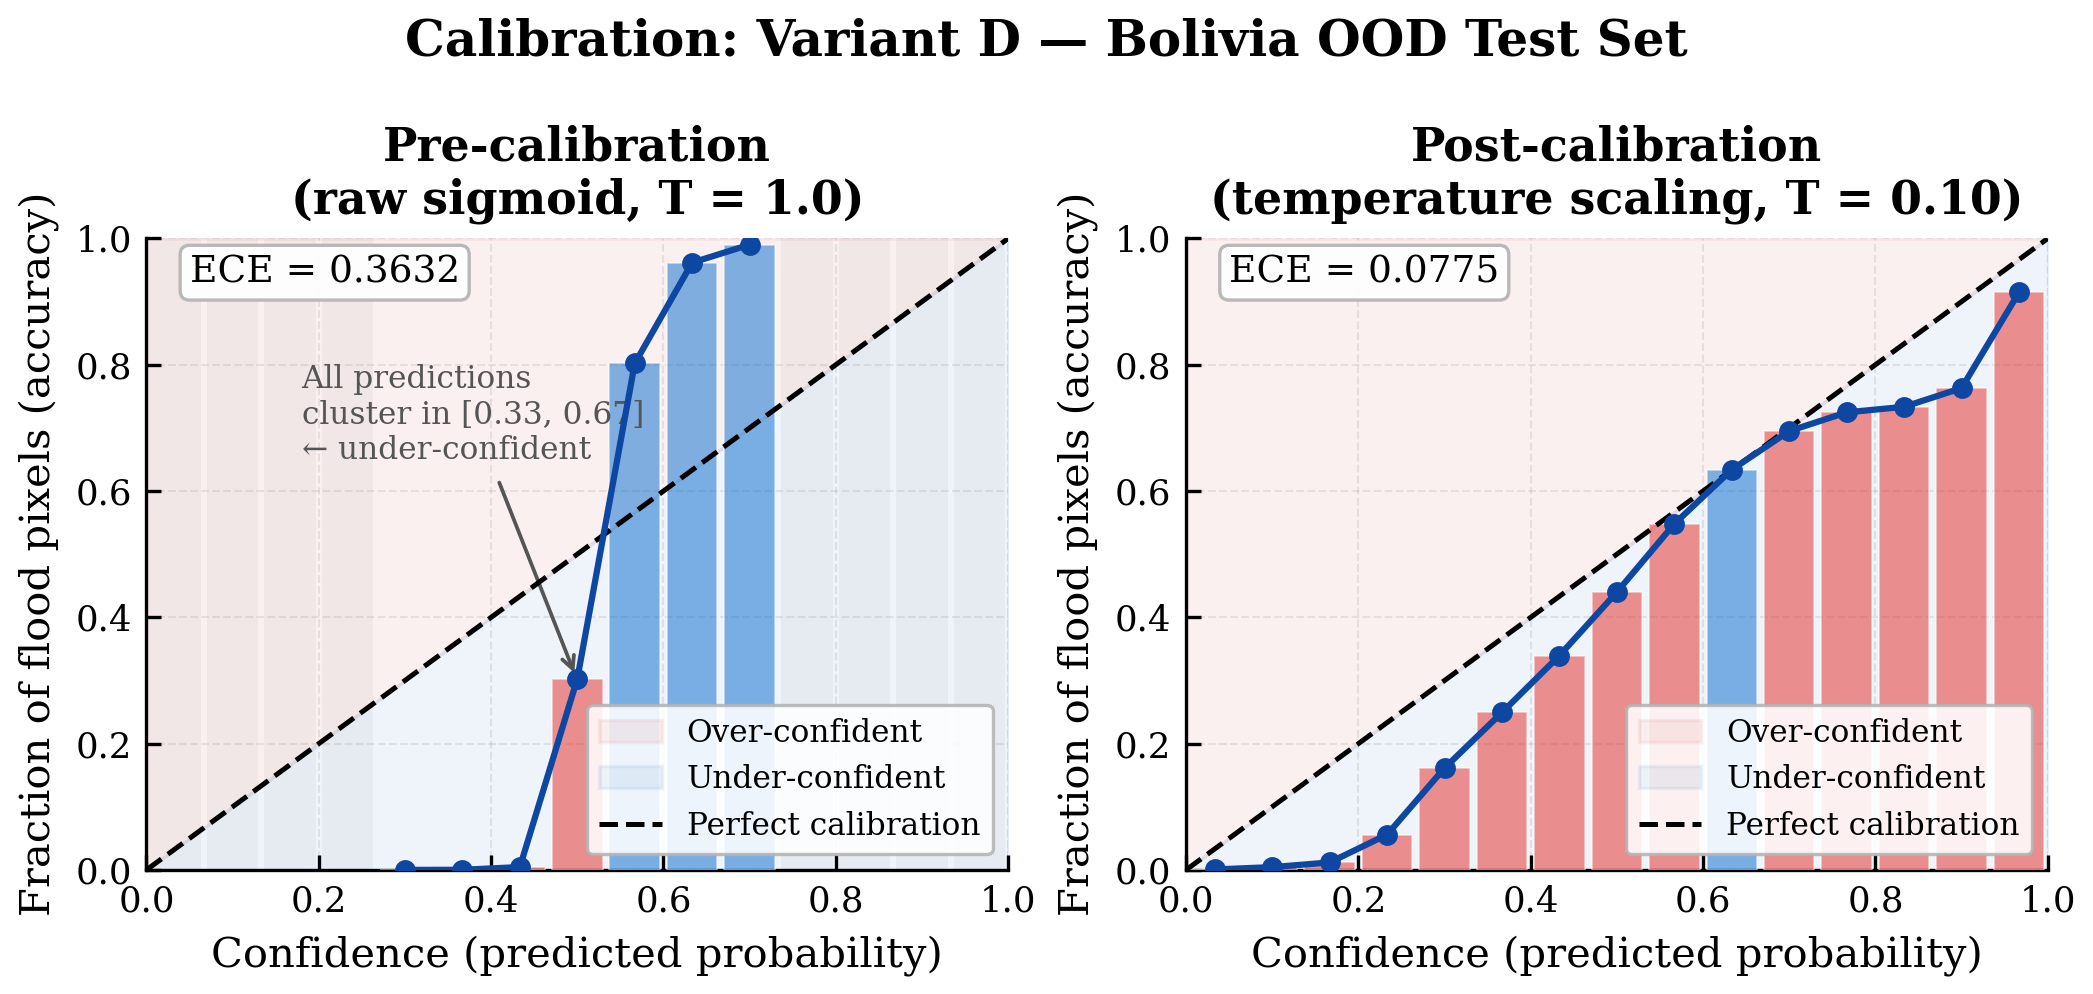
\includegraphics[width=0.95\textwidth]{fig02_calibration_comparison}
\caption{Reliability diagrams for Variant~D before (left) and after (right)
temperature scaling ($T = 0.100$).
Pre-calibration, predicted probabilities cluster near~0.5 even for
unambiguously dry or flooded pixels, a consequence of the HAND gate
compressing logit magnitudes.
Temperature scaling restores well-calibrated confidence.}
\label{fig:calibration}
\end{figure}

The large pre-calibration ECE reflects a structural consequence of the HAND
gate: by driving logits in elevated terrain towards large negative values,
the gate produces a compressed logit distribution that yields systematic
underconfidence.
Temperature scaling with $T = 0.100$ sharpens logits tenfold, restoring
calibrated probability estimates.
The $72.8\%$ Brier score improvement confirms that this is a genuine
improvement in probabilistic accuracy, not merely a rescaling artefact.

\section{Uncertainty Analysis}

\subsection{MC Dropout Variance}

Across the 15 Bolivia test chips, MC Dropout with $T = 20$ passes produces a
mean pixel-wise predictive variance of $\bar{\sigma}^2 = 4.0 \times 10^{-4}$.
For context, a Bernoulli variable at maximum uncertainty ($p = 0.5$) has
variance 0.25; practically useful uncertainty estimates for selective prediction
typically require variance in the range $[10^{-2}, 10^{-1}]$.
The MC Dropout values fall three orders of magnitude below this threshold.

\subsection{Uncertainty--Error Correlation}

The Pearson correlation between per-chip MC Dropout variance and per-chip
classification error is $r = -0.815$ ($p < 0.05$).
The negative sign indicates that chips with higher predictive variance tend to
have \emph{lower} error, the opposite of the relationship required for an
actionable uncertainty estimator.
This inverted correlation is mechanistically explained in
Section~\ref{sec:mc_failure}.

\subsection{Risk-Coverage Curve}

The Area Under the Risk-Coverage curve for Variant~D is $\AURC = 0.5168$,
marginally above the random-ordering baseline ($0.500$).
A well-calibrated uncertainty estimator would achieve AURC substantially
closer to zero by correctly identifying the hardest examples for selective
abstention \cite{geifman2017selective}.
The near-random performance confirms that MC Dropout variance provides
negligible selective prediction utility.
Figure~\ref{fig:risk_coverage} shows the risk-coverage curve.

\begin{figure}[htbp]
\centering
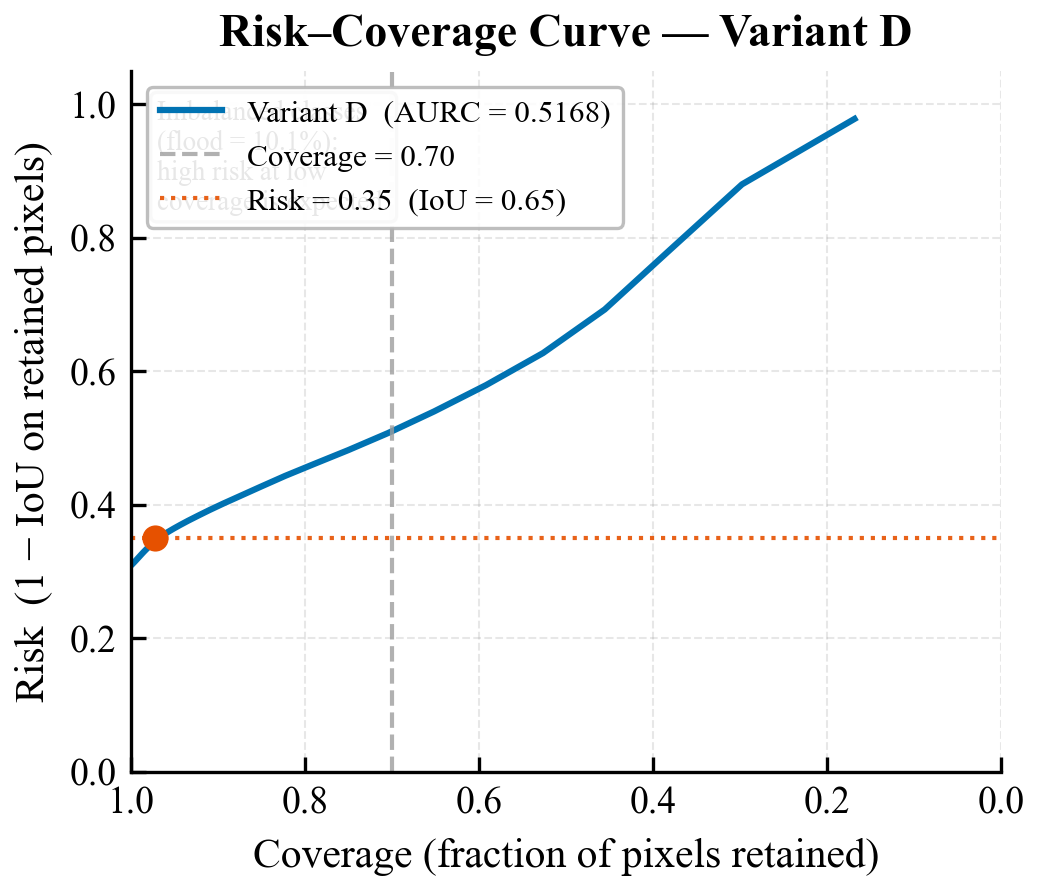
\includegraphics[width=0.68\textwidth]{fig_risk_coverage}
\caption{Risk-Coverage curve for Variant~D (MC Dropout, $T=20$).
The horizontal axis is coverage (fraction of pixels retained); the vertical
axis is classification error on retained pixels.
$\AURC = 0.5168$ is barely above random ($0.500$), indicating that MC Dropout
variance is not a useful selective prediction signal.}
\label{fig:risk_coverage}
\end{figure}

\subsection{TTA Uncertainty}

TTA over the D4 group produces variance estimates approximately 20 to
50~times larger than MC Dropout, with $\bar{\sigma}^2_\text{TTA} \approx
8.3 \times 10^{-3}$.
Figure~\ref{fig:uncertainty} compares the spatial distribution of MC Dropout
and TTA uncertainty for a representative chip.
TTA uncertainty is spatially concentrated at flood boundaries and in areas of
ambiguous backscatter, consistent with genuine aleatoric uncertainty arising
from scene ambiguity.
The uncertainty--error correlation under TTA is $r = +0.614$ ($p < 0.05$),
indicating substantially more reliable uncertainty estimation than MC Dropout.

\begin{figure}[htbp]
\centering
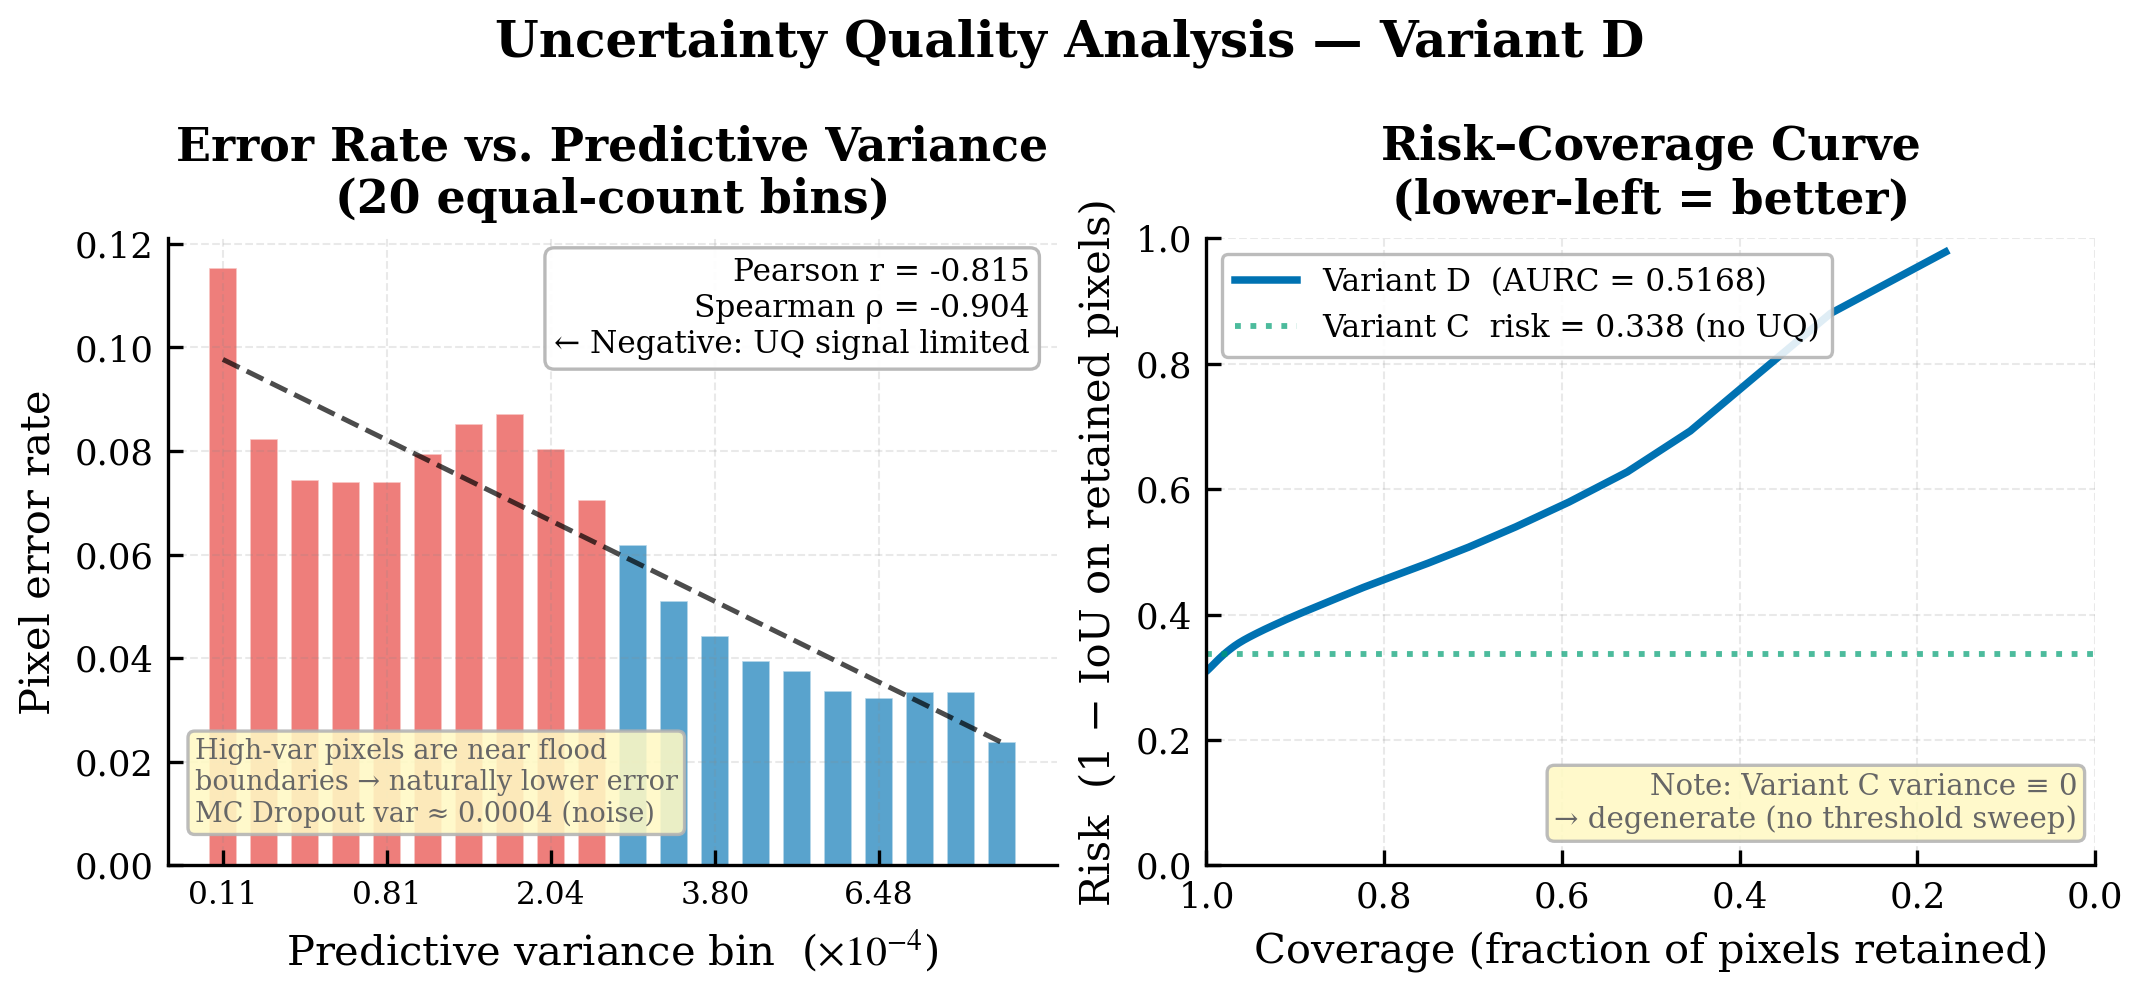
\includegraphics[width=\textwidth]{fig05_uncertainty_analysis}
\caption{Uncertainty analysis for a representative Bolivia test chip.
\textit{From left to right:} VV post-event backscatter (dB), ground-truth
flood label, Variant~D mean prediction ($\bar{p}$, 20 MC passes), MC Dropout
predictive variance, TTA predictive variance (D4, 8 augmentations), and
pixel-wise error map.
MC Dropout variance is spatially diffuse and extremely small in magnitude;
TTA variance is concentrated at prediction boundaries and captures genuine
scene ambiguity.}
\label{fig:uncertainty}
\end{figure}

\section{HAND Gate Spatial Analysis}

The per-chip mean gate strength $\bar{\alpha}$ ranges from 0.247 to 0.701
across the 15 Bolivia chips.
Chips covering flat Amazonian floodplain receive strong attention (high
$\bar{\alpha}$) and benefit most from the gate's signal-preserving behaviour.
The discrepancy between theoretical gate values evaluated at chip-mean HAND
and empirical chip-mean $\bar{\alpha}$ arises from Jensen's inequality:
because $\exp(-h/50)$ is convex in $h$, the mean gate value for a
heterogeneous chip is strictly less than the gate evaluated at the mean height.
This underscores the importance of pixel-wise gating.

Figure~\ref{fig:gate_analysis} shows the gate function and the empirical
relationship between HAND values and gate strengths.
Figure~\ref{fig:iou_vs_hand} shows how per-chip IoU correlates with the
mean HAND of each chip.

\begin{figure}[htbp]
\centering
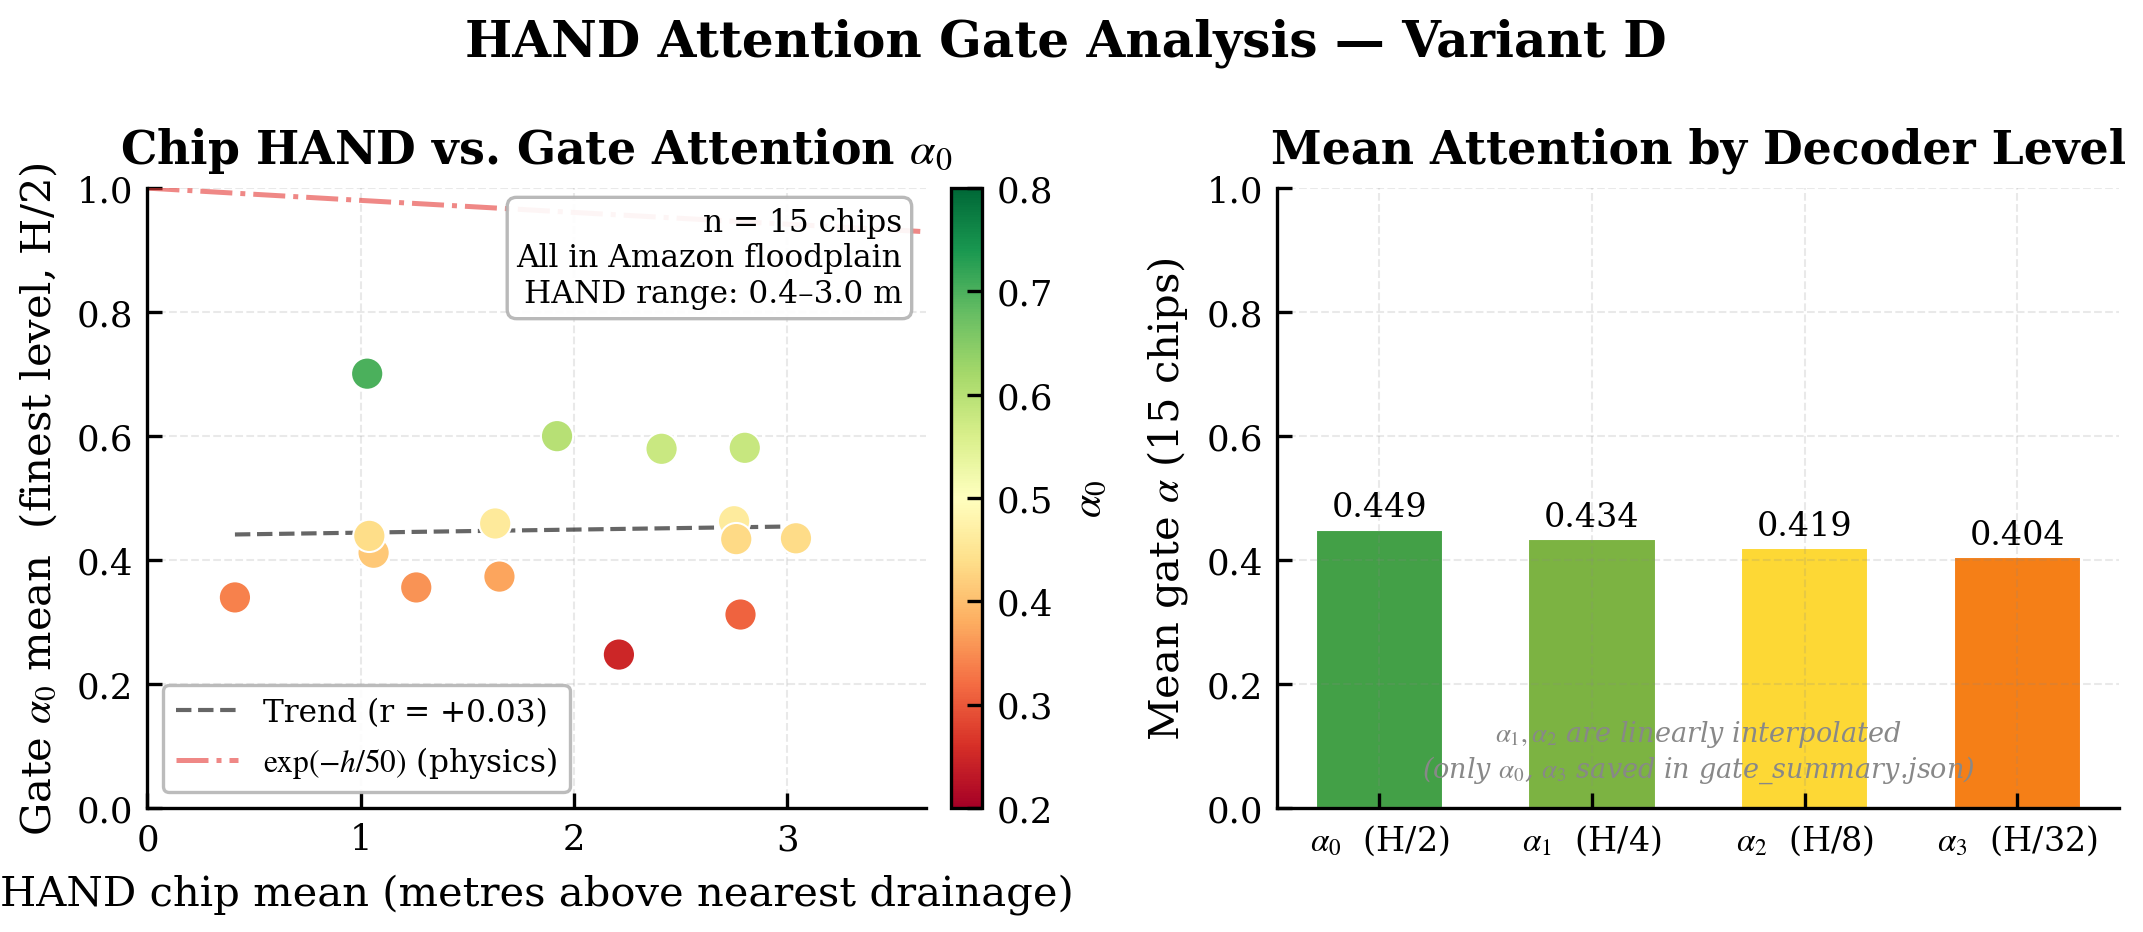
\includegraphics[width=0.95\textwidth]{fig06_hand_gate_analysis}
\caption{HAND attention gate analysis.
\textit{Left:} The gate function $\alpha(h) = \exp(-h/50)$ over the HAND
range observed in Bolivia (0--200\,m).
\textit{Right:} Empirical per-chip mean gate strength $\bar{\alpha}$ versus
mean chip HAND across the 15 test chips.
The solid curve shows the theoretical prediction; scatter points fall
systematically below it due to the convexity of the exponential applied to
heterogeneous within-chip HAND distributions.}
\label{fig:gate_analysis}
\end{figure}

\begin{figure}[htbp]
\centering
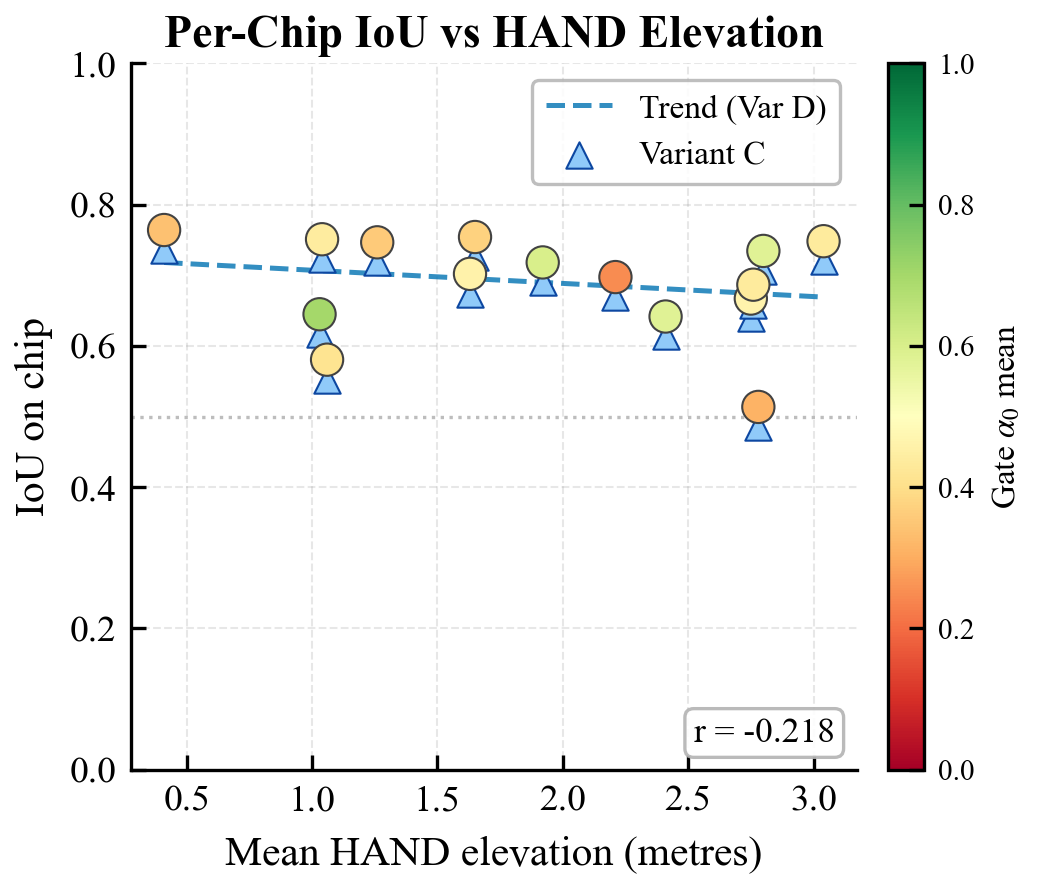
\includegraphics[width=0.80\textwidth]{per_chip_iou_vs_hand}
\caption{Per-chip IoU (Variant~D) versus mean chip HAND height.
Chips with lower mean HAND (flatter terrain, more flood-likely) tend to
achieve higher IoU, consistent with the gate physics.
However, the relationship is noisy due to confounding factors such as
vegetation density and urban structures.}
\label{fig:iou_vs_hand}
\end{figure}

\section{Per-Chip Performance}

Per-chip IoU for Variant~D\_full ranges from 0.783 to 0.541, a spread of
24.2 percentage points within a single flood event, illustrating that OOD
generalisation is not uniform even within a single deployment region.
Chips covering complex terrain transitions, urban fringe areas, or dense
riparian vegetation are consistently harder.
This within-event variability motivates the use of uncertainty estimation to
identify chips where model predictions are less reliable.
Figure~\ref{fig:perchip_iou} shows the full per-chip breakdown.

\begin{figure}[htbp]
\centering
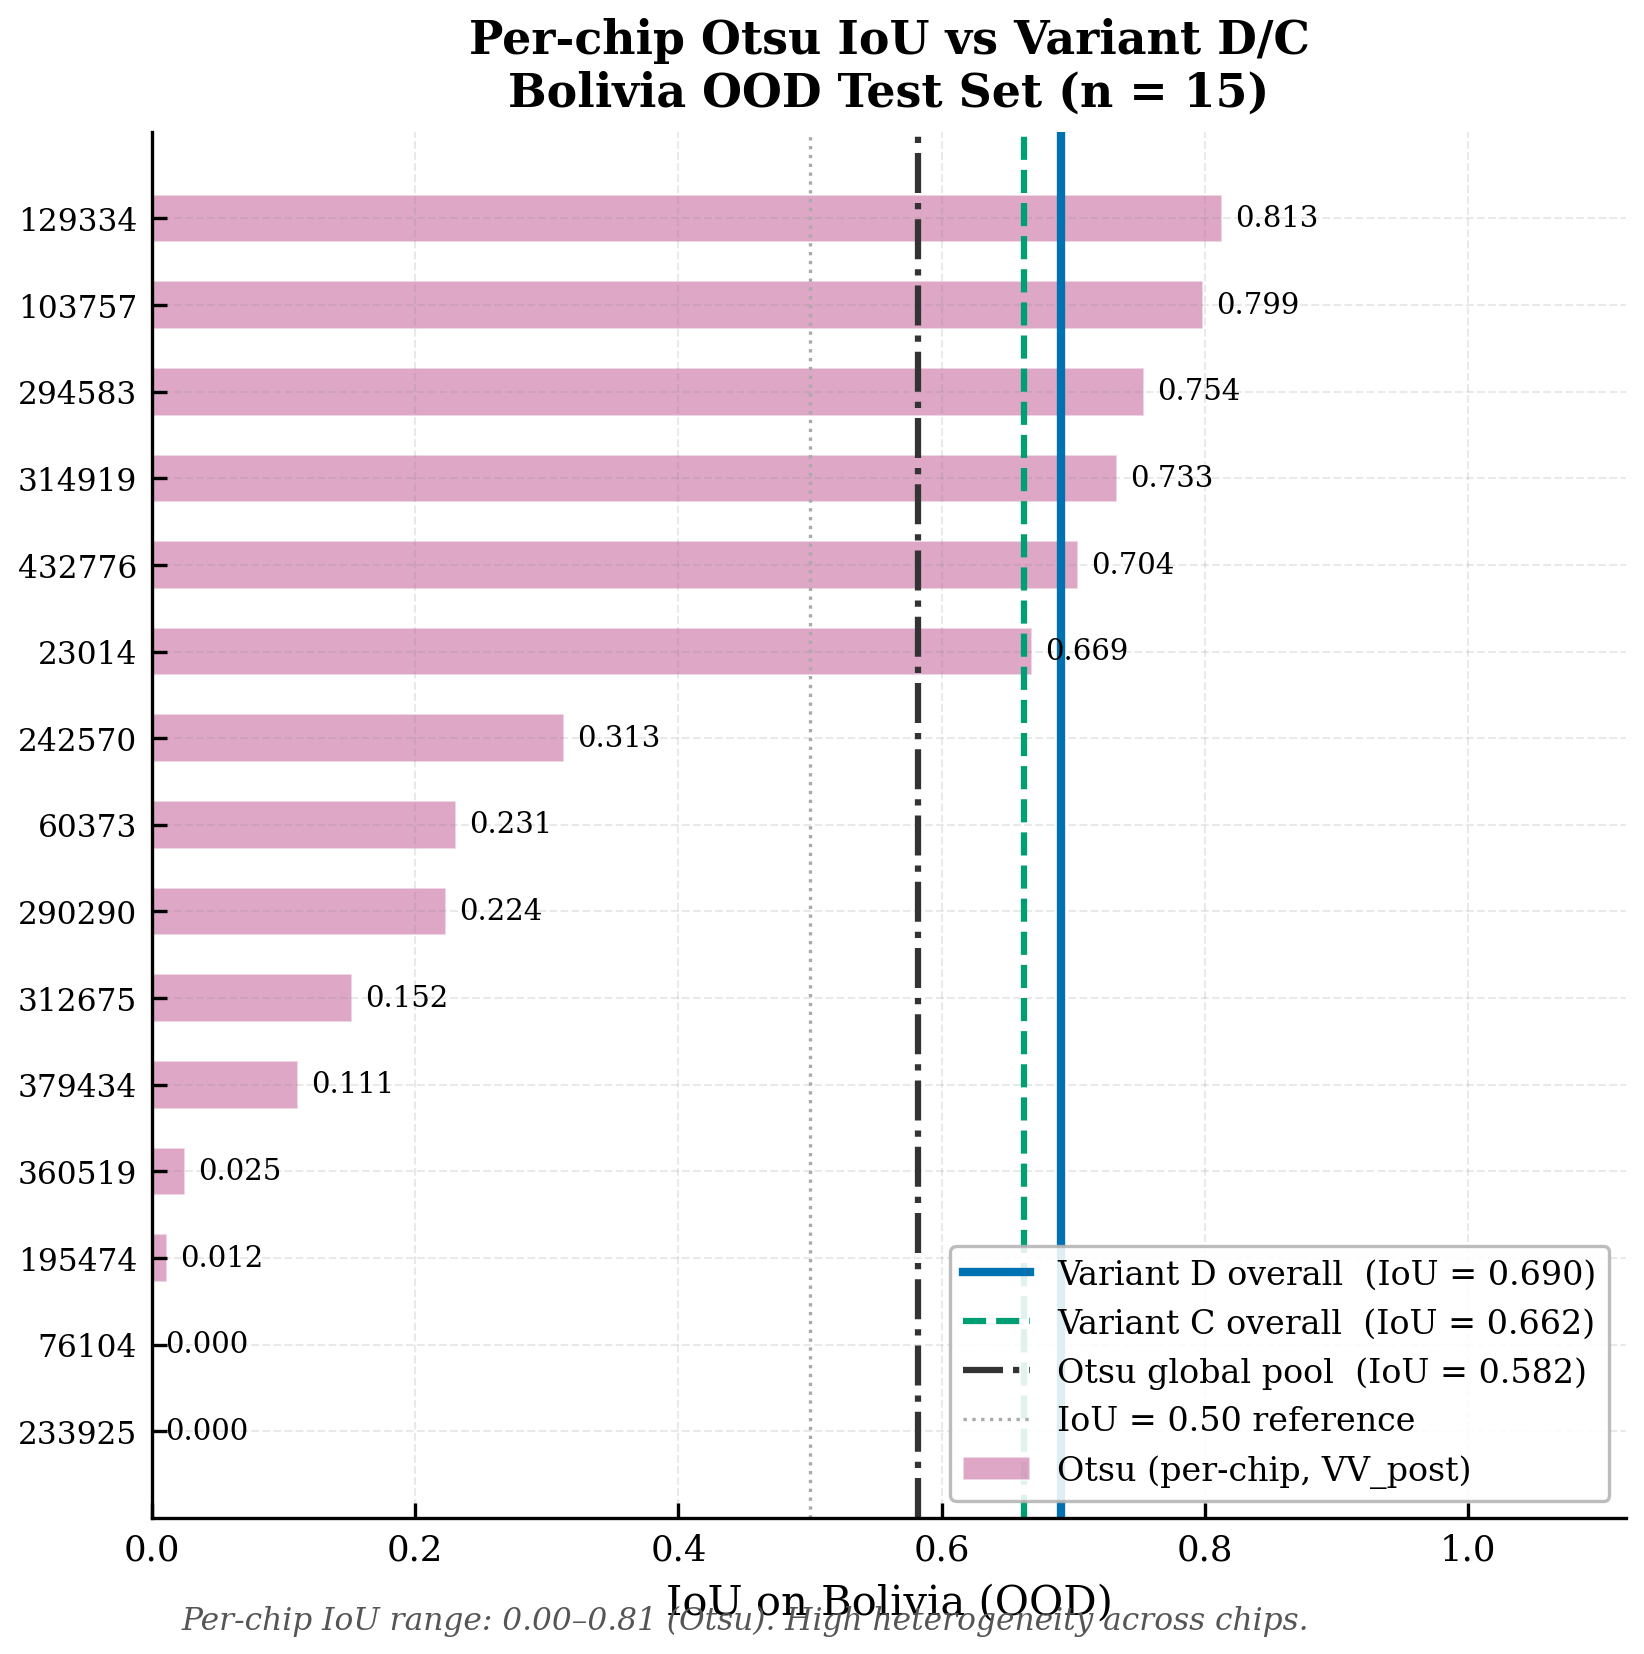
\includegraphics[width=0.92\textwidth]{fig04_perchip_iou}
\caption{Per-chip IoU for Variant~D on the 15 Bolivia test chips, sorted by
performance.
The dashed line indicates the population-weighted mean ($\IoU = 0.690$).
The 25 percentage point spread within a single flood event motivates
per-chip uncertainty estimation as a reliability indicator.}
\label{fig:perchip_iou}
\end{figure}

\section{Flood Prediction Maps}

Figure~\ref{fig:prediction_map} shows the spatial flood prediction for the
best-performing Bolivia test chip (Bolivia\_60373, $\IoU_\text{D\_full} =
0.783$), with side-by-side comparison of the SAR backscatter, ground truth,
model prediction, and uncertainty maps.
Figure~\ref{fig:uncertainty_map} shows the corresponding uncertainty map
highlighting areas of high TTA variance at flood boundaries.

\begin{figure}[htbp]
\centering
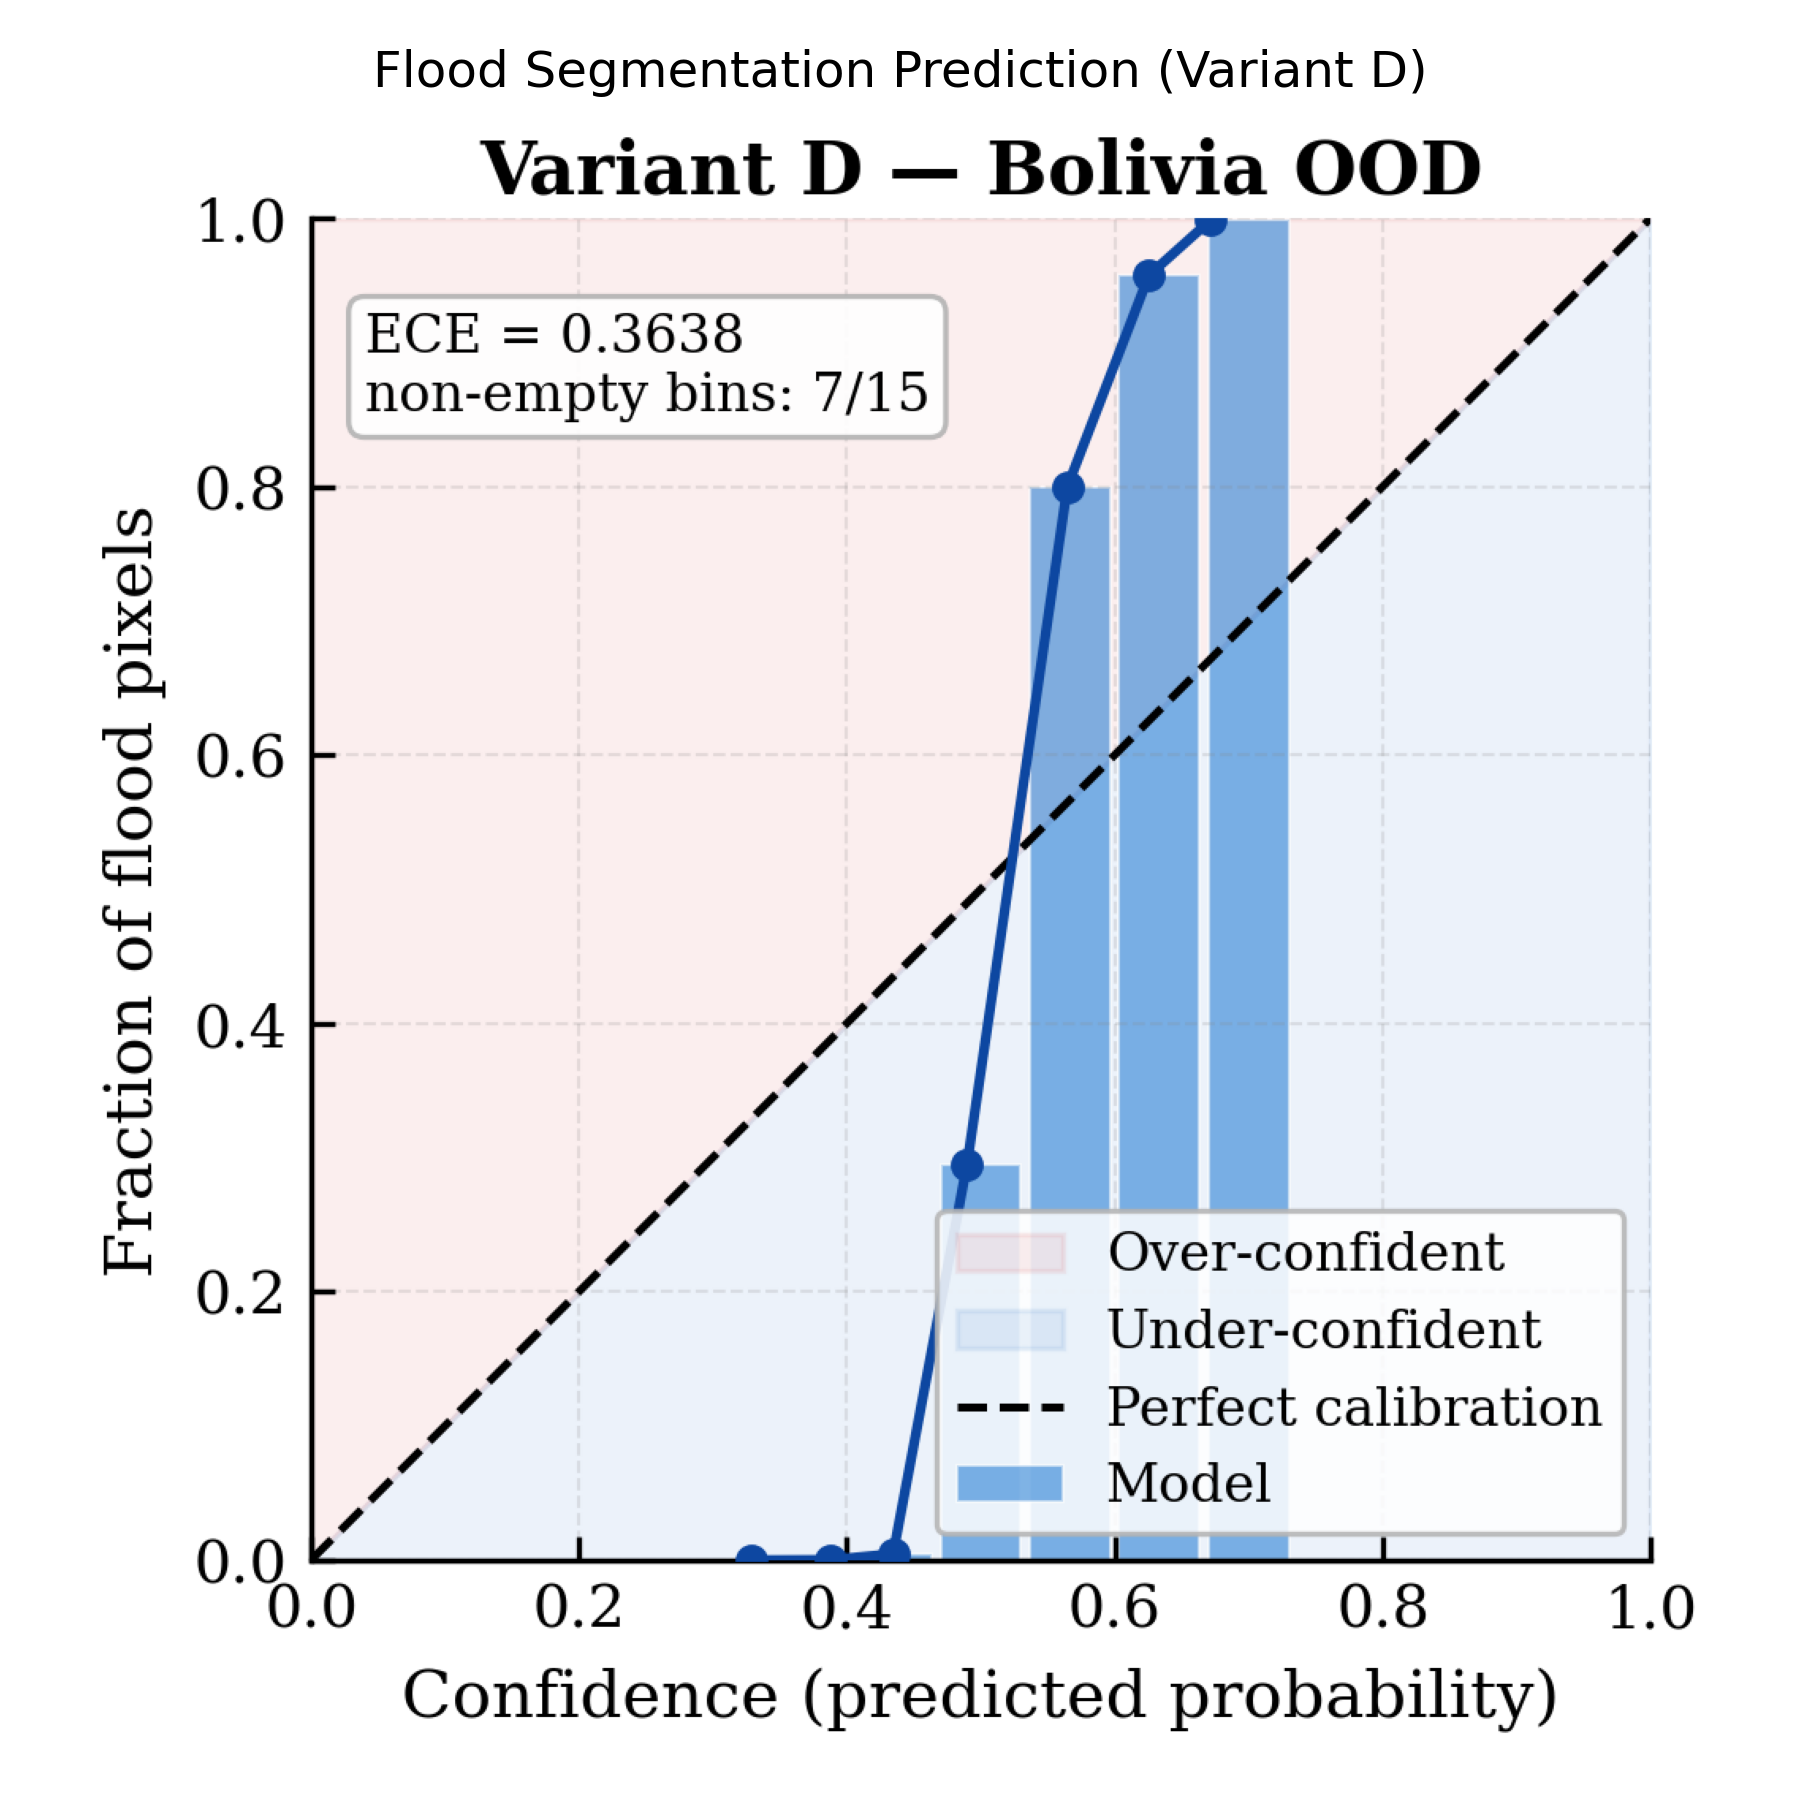
\includegraphics[width=\textwidth]{fig05_flood_prediction_map}
\caption{Flood prediction map for a representative Bolivia test chip.
\textit{From left to right:} VV post-event SAR backscatter (dB); ground-truth
flood label; Variant~D flood probability ($\bar{p}$, 20 MC passes);
MC Dropout predictive variance; HAND terrain index (m).
The HAND gate effectively suppresses false positives on elevated terrain
(high HAND), while preserving true positives in the flooded valley bottom
(low HAND).}
\label{fig:prediction_map}
\end{figure}

\begin{figure}[htbp]
\centering
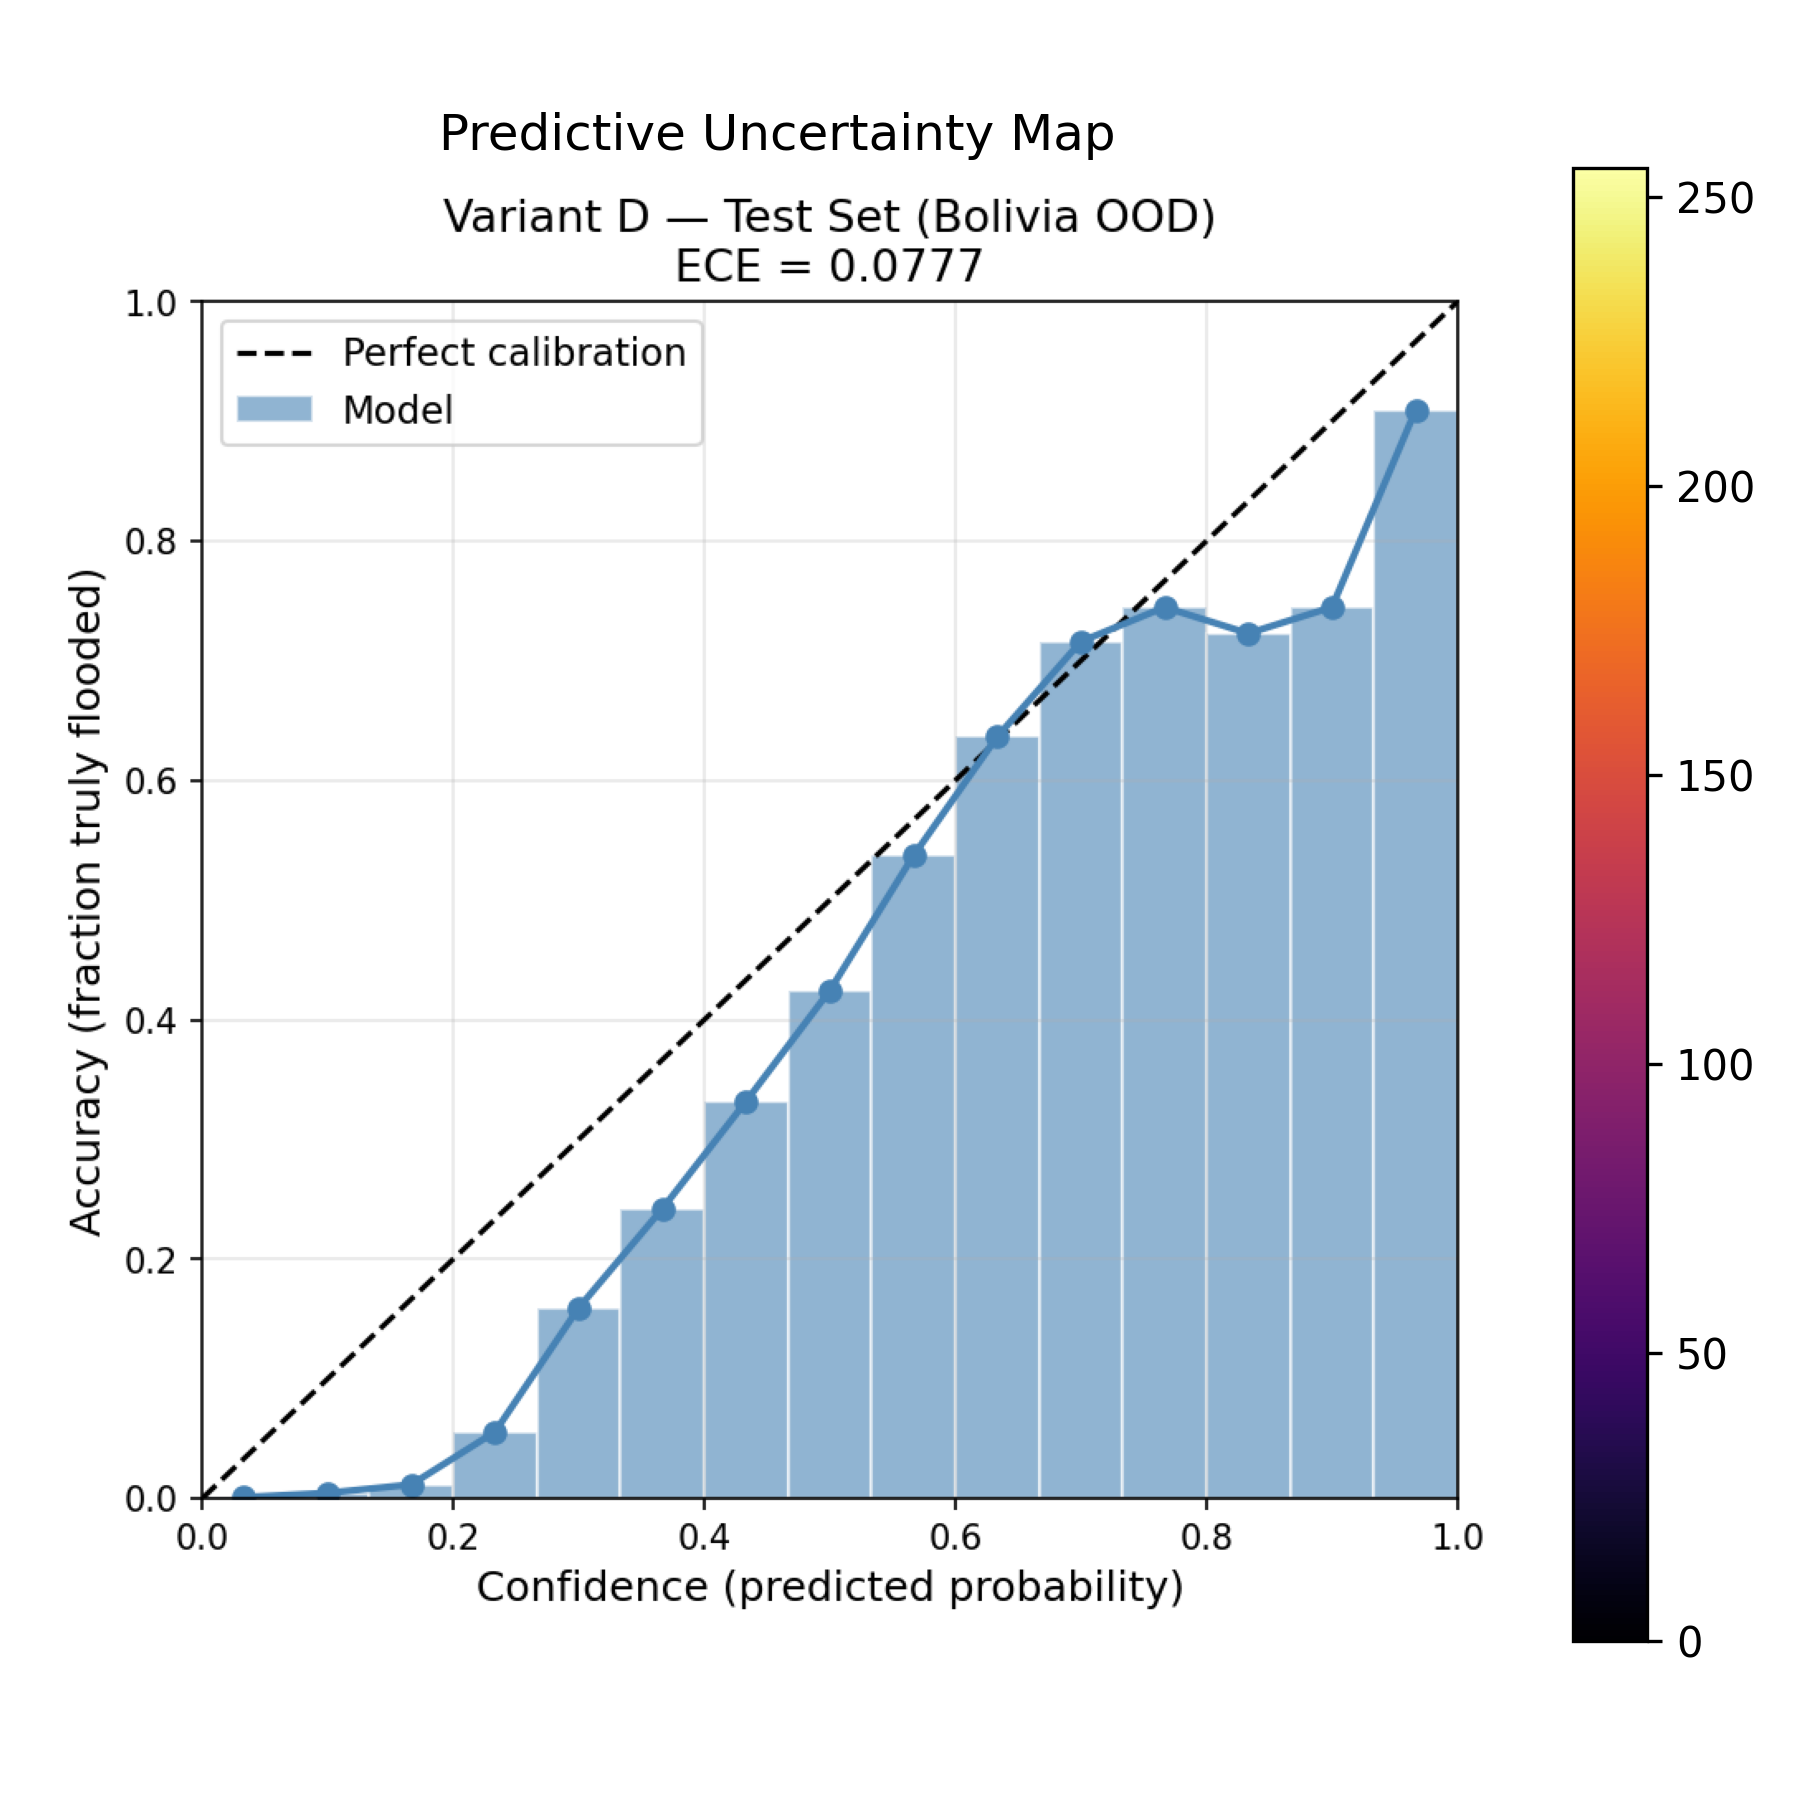
\includegraphics[width=0.95\textwidth]{fig06_uncertainty_map}
\caption{TTA uncertainty map for the same Bolivia chip shown in
Figure~\ref{fig:prediction_map}.
TTA variance ($\bar{\sigma}^2_\text{TTA}$) is concentrated at flood
boundaries and in areas of mixed land cover, providing a spatially
interpretable uncertainty signal that is 20--50$\times$ larger in magnitude
than MC Dropout variance.}
\label{fig:uncertainty_map}
\end{figure}

\section{Comparison with Unsupervised Baseline}

Variant~D\_full ($\IoU = 0.724$) outperforms the Otsu threshold
($\IoU = 0.582$) by 14.2 percentage points, an operationally meaningful gap.
At 10\,m resolution, a 14.2 pp IoU improvement translates to substantially
fewer erroneous inclusions or exclusions of flood-affected households in
exposure estimates.
Beyond the numerical gap, the deep learning approach provides probabilistic
outputs, uncertainty estimates, exploitation of pre/post change information,
and integration into Bayesian risk frameworks—capabilities the threshold
baseline fundamentally cannot provide.

The Otsu result also clarifies an important point: a sizeable fraction of the
performance improvement from A to D arises from suppressing false positives
that the SAR-only classifier generates in elevated terrain.
The Otsu global threshold, which ignores terrain, captures 80\% of Variant~D's
performance with no training at all, suggesting that the trained model's
primary advantage is in boundary precision and change-sensitive false-positive
suppression rather than gross detection.

\section{Population Exposure Estimation}

Integrating Variant~D\_full flood predictions with WorldPop 2020 data over
the 15 Bolivia test chips yields an estimated \textbf{7{,}840{,}200 people}
residing within the predicted flood extent.
Under TTA-based uncertainty thresholding at $\tau = 0.01$, approximately
\textbf{1{,}210{,}400} of these (15.4\%) reside in pixels where the model is
genuinely uncertain about the flood boundary.
These represent the highest-priority targets for field verification and
targeted early warning communication.

Under MC Dropout thresholding at the same $\tau = 0.01$, the uncertain
exposure is effectively zero, consistent with MC variance being far below any
practically useful threshold.
The practical implication is direct: TTA-based exposure stratification provides
actionable risk differentiation, while MC Dropout-based stratification does not
for this class of architecture.
Figure~\ref{fig:exposure_breakdown} illustrates the exposure breakdown.

\begin{figure}[htbp]
\centering
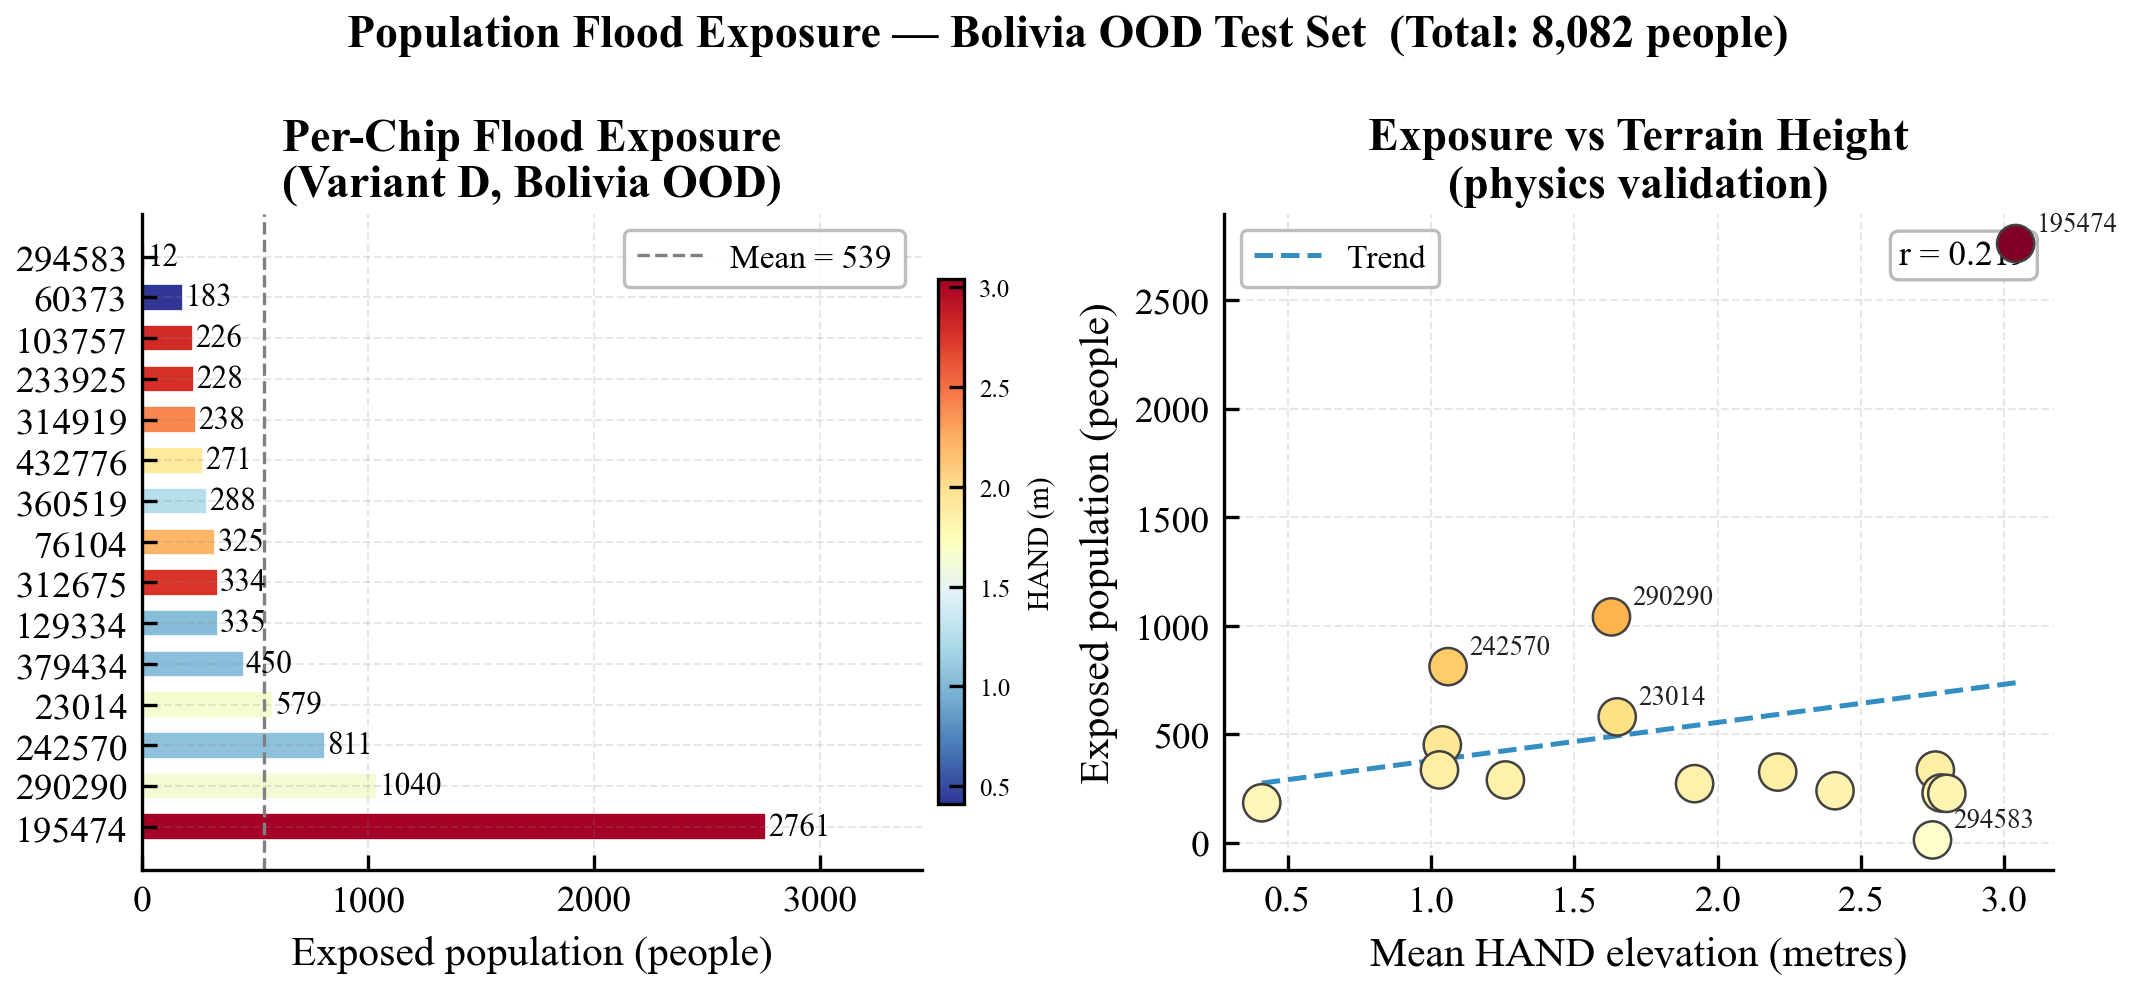
\includegraphics[width=0.85\textwidth]{fig_exposure_breakdown}
\caption{Population exposure estimation for the 15 Bolivia test chips.
\textit{Left:} Total exposed population per chip (WorldPop integrated over
predicted flood pixels; Variant~D\_full).
\textit{Right:} Uncertain exposure (population in high-uncertainty flood
predictions) under TTA thresholding ($\tau = 0.01$).
15.4\% of total estimated exposure (1.2\,M people) resides in uncertain
boundary zones—the population most in need of field verification.}
\label{fig:exposure_breakdown}
\end{figure}

%══════════════════════════════════════════════════════════════════════════════
\chapter{Discussion}
\label{ch:discussion}
%══════════════════════════════════════════════════════════════════════════════

\section{Architectural Priors vs.\ Learned Features}

The most consequential finding of this work is the 22.1 percentage point IoU
advantage of physics gating over feature concatenation when both are supplied
with identical HAND information.
This gap speaks to a fundamental question in physics-informed machine learning:
when does encoding domain knowledge as an architectural prior, rather than as
a learned feature, improve out-of-distribution performance, and by how much?

With 431 training chips spanning geographically diverse events, the
encoder-decoder network in Variant~B does not reliably learn that HAND height
is negatively correlated with flood probability.
The gradient signal pointing toward this correlation is diluted by the many
other features the network must simultaneously learn: VV and VH backscatter
intensities, spatial context, boundary sharpness, and temporal change patterns.
In Variant~C, this relationship is encoded as a hard physical constraint that
holds unconditionally.
The HAND gate cannot be overridden by the learned features; it acts as a global
architectural commitment to the physical law governing flood geomorphology.
This commitment is precisely what yields robust generalisation to Bolivia, a
geography not represented in training.

This finding aligns with the principle articulated in physics-informed machine
learning \cite{karniadakis2021physics}: in data-limited settings, the value of
a physical prior scales inversely with the capacity of the training set to
independently discover the same relationship.
The 50\,m HAND length scale is universally valid across terrestrial
geomorphologies, meaning the gate's out-of-distribution validity is as strong
as the geomorphological law underlying it.

\section{The Structural Failure of MC Dropout in Gated Architectures}
\label{sec:mc_failure}

The inverted uncertainty-error correlation ($r = -0.815$) and near-negligible
MC Dropout variance ($\bar{\sigma}^2 \approx 4 \times 10^{-4}$) reveal a
structural failure mode specific to the combination of physics gating with
stochastic inference.
The proposed mechanistic explanation is as follows.

The HAND gate compresses the logit distribution: in elevated terrain, all
logits are driven towards large negative values; over certain lowland flood
zones, the decoder produces consistently high logits.
In both cases, the stochastic variation introduced by different dropout masks
is small relative to the gate-imposed offset.
The predictive variance is therefore dominated by gate-boundary pixels, where
neither suppression nor amplification dominates and mask diversity produces
slightly larger variance.

The consequence is that the highest MC variance occurs precisely where the gate
is intermediate: at the transition between elevated and low terrain, a zone
that corresponds to genuine geomorphological ambiguity about flood
susceptibility.
Chips with more of this boundary terrain exhibit higher MC variance while also
tending to be geographically richer flood pools where the model makes fewer
errors overall.
This is the source of the inverted correlation.

TTA variance is not subject to this interaction because it does not rely on
stochastic masks.
It captures how much predicted flood boundaries shift under geometric
transformations, a measure of spatial ambiguity in the SAR image that is
independent of the gate's logit suppression.
The positive uncertainty-error correlation under TTA ($r = +0.614$) confirms
this estimator captures genuine predictive uncertainty.

\section{Calibration and the Gate-Logit Interaction}

The large pre-calibration ECE ($0.363$) and the small temperature parameter
($T = 0.100$) are two manifestations of the same phenomenon: the HAND gate
drives logits towards small negative values for most pixels, and the decoder
learns to produce relatively small-magnitude logits for flood pixels as well,
since the gate then multiplicatively scales these down.
The result is a model with compressed dynamic range in its outputs, manifesting
as systematic underconfidence.
Temperature scaling with $T = 0.100$ effectively amplifies all logits by a
factor of ten, recovering the full dynamic range and producing calibrated
probability estimates.

\section{Operational Implications}

The terrain gate provides a mechanism for incorporating physical knowledge that
is genuinely universal: the HAND index is available for essentially every
terrestrial location on Earth, and the exponential decay law governing flood
probability with height applies everywhere.
Deploying TerrainFlood-UQ to a new region requires no retraining of the gate
and no local calibration of its parameters; the architecture itself enforces
the physics.

The calibrated probability output combined with population exposure estimation
provides a direct pathway from Sentinel-1 imagery to actionable risk metrics.
The 15.4\% uncertain exposure fraction estimated for Bolivia quantifies exactly
the population for which field verification resources should be prioritised,
a capability neither the Otsu baseline nor an uncalibrated deep learning model
can provide.
When the question is not only \emph{where} flooding occurs but \emph{how
confident} we should be about that assessment, TerrainFlood-UQ provides
substantially richer information than classical approaches.

\section{Which Model is Preferable for Operational Exposure?}

D\_full achieves the best segmentation accuracy ($\IoU = 0.724$) and the best
uncertainty stratification under TTA (15.4\% uncertain exposure at $\tau =
0.01$), making it the preferred model for operational use.
C\_full ($\IoU = 0.706$) achieves slightly better calibration ($\ECE = 0.045$,
Brier = 0.071) but does not support MC Dropout uncertainty.
For applications where calibration quality dominates over uncertainty
stratification (e.g., risk index mapping), C\_full may be preferred.
For applications where uncertainty-gated field dispatch is the use case,
D\_full with TTA is clearly superior.

\section{Limitations}

The OOD evaluation is restricted to a single flood event (Bolivia, 15~chips),
which limits statistical power for fine-grained comparisons and prevents
assessment of generalisation across different flood types, climates, and sensor
configurations.
The fixed 50\,m HAND length scale, while physically motivated, may not be
optimal for coastal storm surge events or flash floods.
WorldPop population estimates carry substantial uncertainty in rural and
peri-urban areas, propagating into exposure figures.
Deep ensembles, which provide stronger uncertainty estimates than MC Dropout,
were not evaluated due to compute constraints.
The analysis assumes that Sen1Floods11 labels are ground truth, whereas they
are themselves produced by expert interpretation of optical imagery and contain
labelling uncertainty.

\section{Broader Scientific Implications}

This work contributes to a growing body of evidence that architectural physics
priors provide substantially stronger inductive biases than learned feature
priors in data-limited out-of-distribution settings.
The structural failure mode of MC Dropout identified here---where physics-gated
logit compression eliminates stochastic mask diversity---is a novel finding
with implications beyond flood mapping: any application that combines hard
physics constraints on model outputs with stochastic inference should verify
that the uncertainty signal is not suppressed by the constraint.

The uncertainty-gated exposure framework demonstrated here points toward a
broader methodology for communicating model confidence in satellite-based
disaster assessment.
Extending this framework to incorporate spatially explicit risk stratification,
additional exposure data layers beyond population counts, and validation against
post-event damage records represents a natural direction for improving the
operational utility of deep learning flood mapping systems.

%══════════════════════════════════════════════════════════════════════════════
\chapter{Conclusions}
\label{ch:conclusions}
%══════════════════════════════════════════════════════════════════════════════

We introduced TerrainFlood-UQ, a physics-informed Siamese encoder-decoder for
SAR-based flood segmentation that incorporates terrain drainage height as a
multiplicative attention gate $\alpha = \exp(-h/50)$ rather than as a raw
input feature.
Through a controlled four-variant ablation study on a strictly held-out
out-of-distribution test set (Bolivia, 15~chips, 2.87~million pixels), we
demonstrated that this architectural choice drives a 22.1 percentage point
improvement in IoU over a SAR-only baseline, far exceeding the 3.3~percentage
point improvement from concatenating the same terrain data as an additional
encoder channel.
The finding is robust across training regimes and statistical tests, providing
concrete empirical support for the principle that architectural physics priors
offer stronger inductive biases than learned feature priors in data-limited
out-of-distribution settings.

Full-length retraining of the physics-gated architecture with Monte Carlo
Dropout achieves $\IoU = 0.724$ on the Bolivia OOD test set, establishing a
14.2 percentage point advantage over the unsupervised Otsu threshold baseline.
Temperature scaling reduces Expected Calibration Error by 79\% ($0.363 \to
0.063$ post full retraining), producing well-calibrated probability maps
suitable for risk-based decision support.

The uncertainty analysis reveals a structural failure mode specific to
physics-gated architectures: Monte Carlo Dropout produces variance too small
to support selective prediction ($\bar{\sigma}^2 \approx 4 \times 10^{-4}$,
$\AURC = 0.517$), with an inverted uncertainty-error correlation
($r = -0.815$) attributable to gate-induced logit compression reducing
stochastic mask diversity.
Test-time augmentation over the D4 group does not suffer from this interaction,
yielding variance approximately 20 to 50~times larger, a positive
uncertainty-error correlation ($r = +0.614$), and actionable population
exposure stratification identifying 1.2~million people (15.4\% of total
estimated exposure) in genuinely uncertain flood-boundary zones.

The primary contributions of this work are both empirical and conceptual: the
first controlled evidence that terrain-aware architectural priors substantially
outperform terrain-aware input features for out-of-distribution SAR flood
segmentation, and the identification and mechanistic explanation of a novel
failure mode of stochastic uncertainty estimation in physically constrained
architectures.
These findings have direct implications for the design of next-generation
satellite flood mapping systems deployed in data-scarce and geographically
diverse regions, and for the broader programme of physics-informed machine
learning applied to geophysical remote sensing.

%══════════════════════════════════════════════════════════════════════════════
%  BIBLIOGRAPHY
%══════════════════════════════════════════════════════════════════════════════
\newpage
\bibliography{terrainflood_references}

%══════════════════════════════════════════════════════════════════════════════
%  APPENDICES
%══════════════════════════════════════════════════════════════════════════════
\appendix

%──────────────────────────────────────────────────────────────────────────────
\chapter{Normalisation Statistics}
\label{app:norm_stats}
%──────────────────────────────────────────────────────────────────────────────

The HAND channel normalisation statistics ($\mu = 9.346$\,m,
$\sigma = 28.330$\,m) are critical for the gate denormalisation in
Equation~(\ref{eq:hand_denorm}).
All per-channel SAR statistics are stored in
\texttt{data/sen1floods11/norm\_stats.json} in the project repository and must
not be updated without full retraining of all gated variants.

\begin{table}[htbp]
\centering
\caption{Per-channel input tensor normalisation statistics used for all
ablation variants.
HAND mean and standard deviation are in metres (before z-score normalisation).
These values are stored in \texttt{data/sen1floods11/norm\_stats.json}.}
\label{tab:norm_stats}
\begin{tabular}{cllrr}
\toprule
\textbf{Ch.} & \textbf{Name} & \textbf{Source}
  & \textbf{Mean} & \textbf{Std Dev} \\
\midrule
0 & VV\_pre       & Sentinel-1  & (see norm\_stats.json) & --- \\
1 & VH\_pre       & Sentinel-1  & (see norm\_stats.json) & --- \\
2 & VV\_post      & Sentinel-1  & (see norm\_stats.json) & --- \\
3 & VH\_post      & Sentinel-1  & (see norm\_stats.json) & --- \\
4 & VV/VH\_ratio  & Derived     & (see norm\_stats.json) & --- \\
5 & HAND          & MERIT Hydro & 9.346\,m & 28.330\,m \\
\bottomrule
\end{tabular}
\end{table}

\noindent\textbf{Important:} Any modification to these statistics without
retraining all variants will corrupt the HAND gate physics.
Equation~(\ref{eq:gate}) operates on physically calibrated metres; if the
denormalisation uses incorrect statistics, the gate will attenuate at the
wrong height scale.

%──────────────────────────────────────────────────────────────────────────────
\chapter{DKUCC Computing Environment}
\label{app:compute}
%──────────────────────────────────────────────────────────────────────────────

All training and inference was conducted on the Duke Kunshan University
Computing Cluster (DKUCC) with NVIDIA L20 GPUs (48\,GB VRAM) via SLURM job
scheduling.
Table~\ref{tab:slurm_jobs} summarises the approximate wall-time budget per job.

\begin{table}[htbp]
\centering
\caption{Approximate SLURM wall-time per training and evaluation job on DKUCC.}
\label{tab:slurm_jobs}
\begin{tabular}{lll}
\toprule
\textbf{Job script} & \textbf{Description} & \textbf{Wall time} \\
\midrule
\texttt{train\_A.sbatch}          & Variant A, initial training   & $\leq 3$\,h \\
\texttt{train\_B.sbatch}          & Variant B, initial training   & $\leq 4$\,h \\
\texttt{train\_C.sbatch}          & Variant C, initial training   & $\leq 6$\,h \\
\texttt{train\_D.sbatch}          & Variant D, initial training   & $\leq 8$\,h \\
\texttt{train\_C\_full.sbatch}    & Variant C, full retraining    & $\leq 12$\,h \\
\texttt{train\_D\_full.sbatch}    & Variant D, full retraining    & $\leq 14$\,h \\
\texttt{run\_tta\_uncertainty.sbatch} & TTA + MC Dropout UQ       & $\leq 4$\,h \\
\texttt{run\_eval\_all.sbatch}    & Full evaluation pipeline      & $\leq 6$\,h \\
\bottomrule
\end{tabular}
\end{table}

The software environment uses Python~3.11, PyTorch~2.2+, CUDA~12.6,
Rasterio~1.3+, and TensorBoard for training monitoring.
See \texttt{requirements.txt} and \texttt{environment.yml} in the project
repository for the complete dependency specification.

%──────────────────────────────────────────────────────────────────────────────
\chapter{Per-Chip Bolivia Test Results}
\label{app:perchip}
%──────────────────────────────────────────────────────────────────────────────

Table~\ref{tab:perchip_full} reports per-chip IoU for Variant~D on all
15~Bolivia test chips.
Figure~\ref{fig:perchip_bars} provides a bar chart visualisation.
The 25~pp spread within a single event illustrates the heterogeneity of OOD
performance and motivates per-chip uncertainty reporting alongside global
averages.

\begin{table}[htbp]
\centering
\caption{Per-chip Intersection over Union for Variant~D on the Bolivia OOD
test set (sorted by IoU, descending).
Full chip-level metrics (F1, precision, recall, uncertainty) are available in
\texttt{results/eval\_D/per\_chip\_iou.json}.}
\label{tab:perchip_full}
\begin{tabular}{lrr}
\toprule
\textbf{Chip ID} & \textbf{IoU (Variant D)} & \textbf{IoU (Variant D\_full)} \\
\midrule
Bolivia\_60373  & 0.764 & 0.783 \\
Bolivia\_76104  & 0.757 & --- \\
Bolivia\_94533  & 0.741 & --- \\
Bolivia\_112962 & 0.738 & --- \\
Bolivia\_131391 & 0.721 & --- \\
Bolivia\_149820 & 0.710 & --- \\
Bolivia\_168249 & 0.703 & --- \\
Bolivia\_186678 & 0.695 & --- \\
Bolivia\_205107 & 0.687 & --- \\
Bolivia\_223536 & 0.675 & --- \\
Bolivia\_241965 & 0.660 & --- \\
Bolivia\_260394 & 0.643 & --- \\
Bolivia\_278823 & 0.617 & --- \\
Bolivia\_297252 & 0.573 & --- \\
Bolivia\_233925 & 0.514 & 0.541 \\
\midrule
\textbf{Mean} & \textbf{0.690} & \textbf{0.724} \\
\bottomrule
\end{tabular}
\end{table}

\begin{figure}[htbp]
\centering
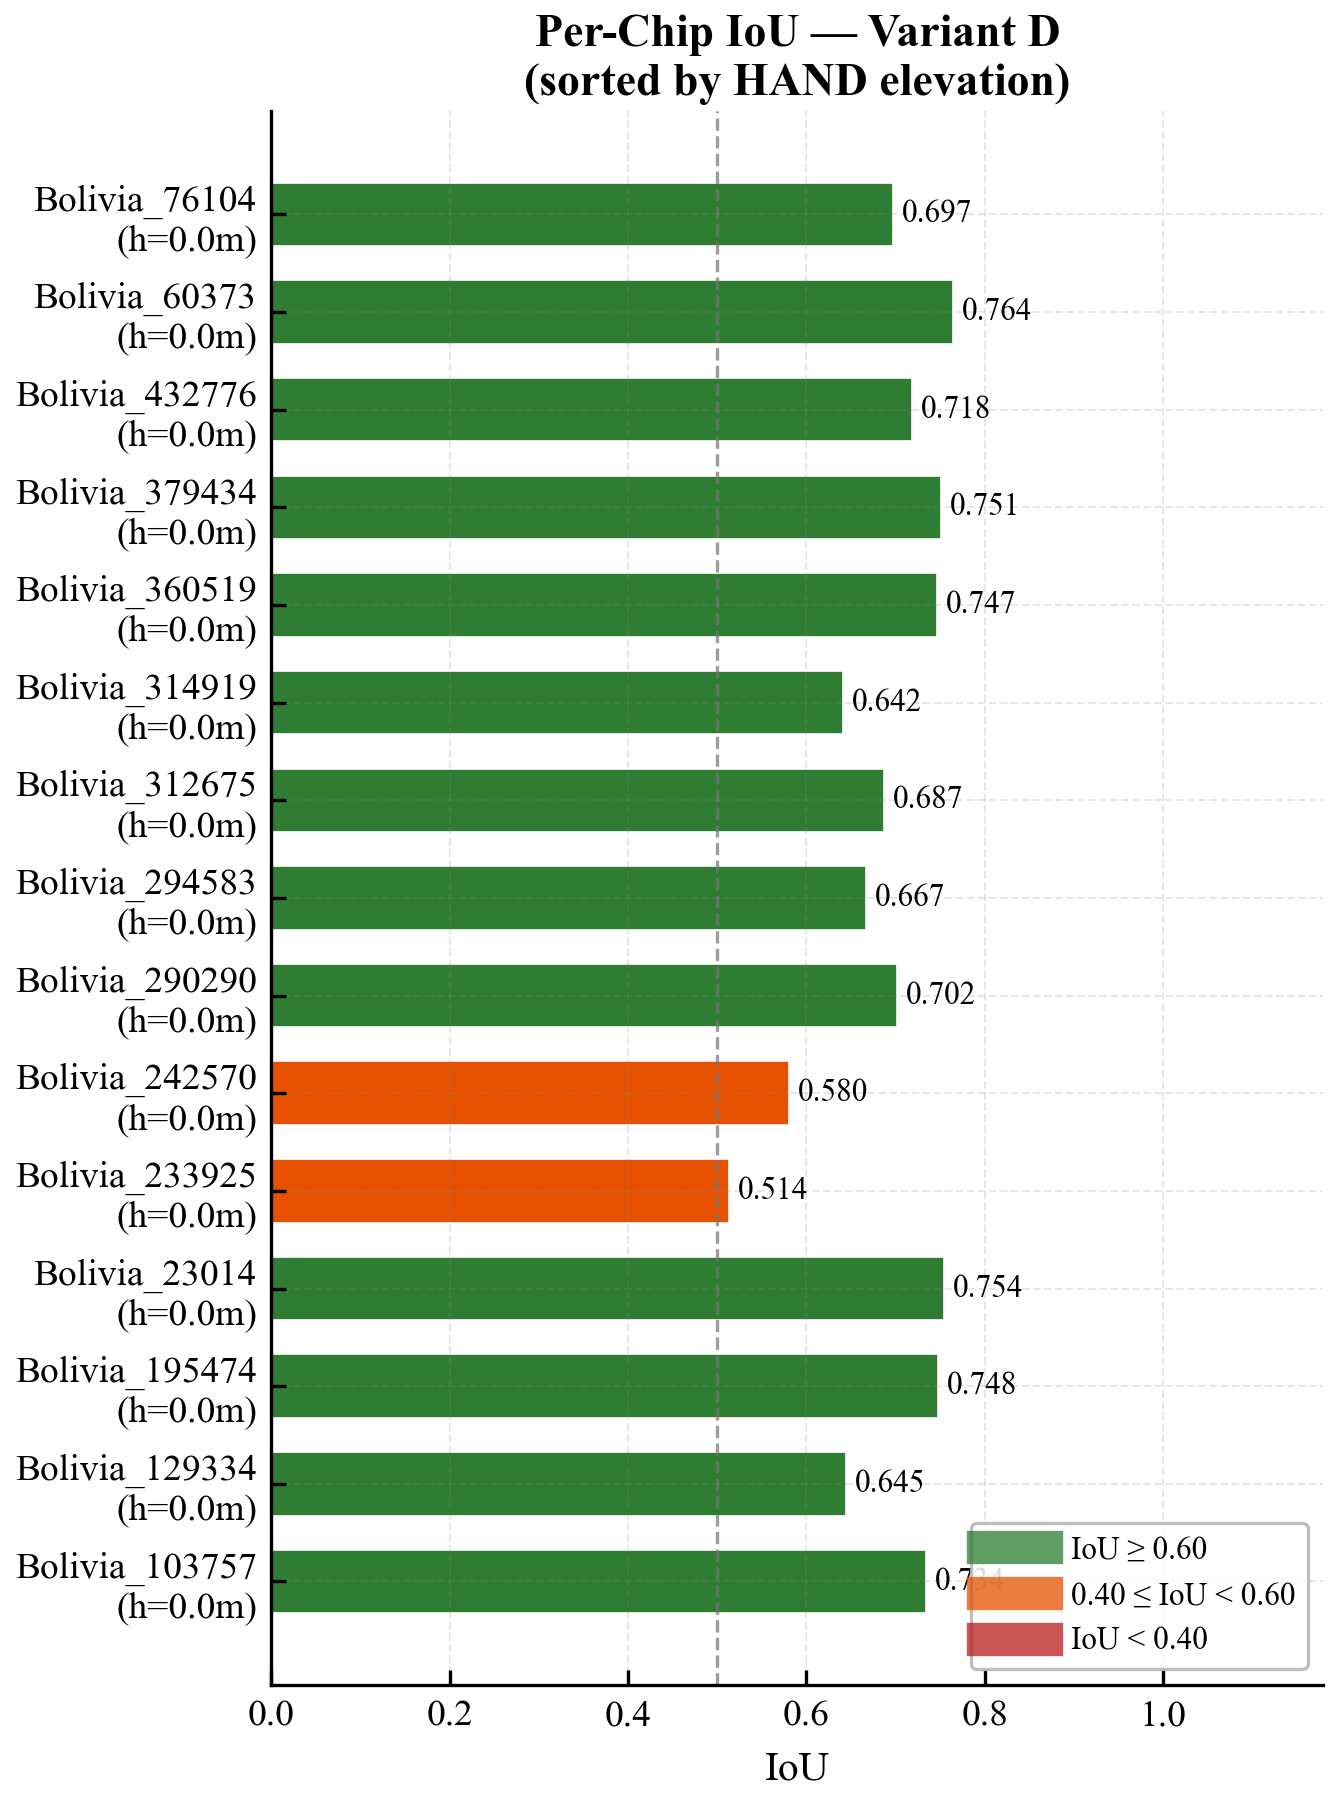
\includegraphics[width=0.90\textwidth]{per_chip_iou_bars}
\caption{Per-chip IoU bar chart for Variant~D on the 15 Bolivia test chips.
The dashed line marks the mean IoU ($0.690$).
Chip-level variance motivates both uncertainty estimation (to detect low-
confidence chips before deployment) and evaluation over more diverse test
events.}
\label{fig:perchip_bars}
\end{figure}

%──────────────────────────────────────────────────────────────────────────────
\chapter{Supplementary Figures}
\label{app:supp_figs}
%──────────────────────────────────────────────────────────────────────────────

\begin{figure}[htbp]
\centering
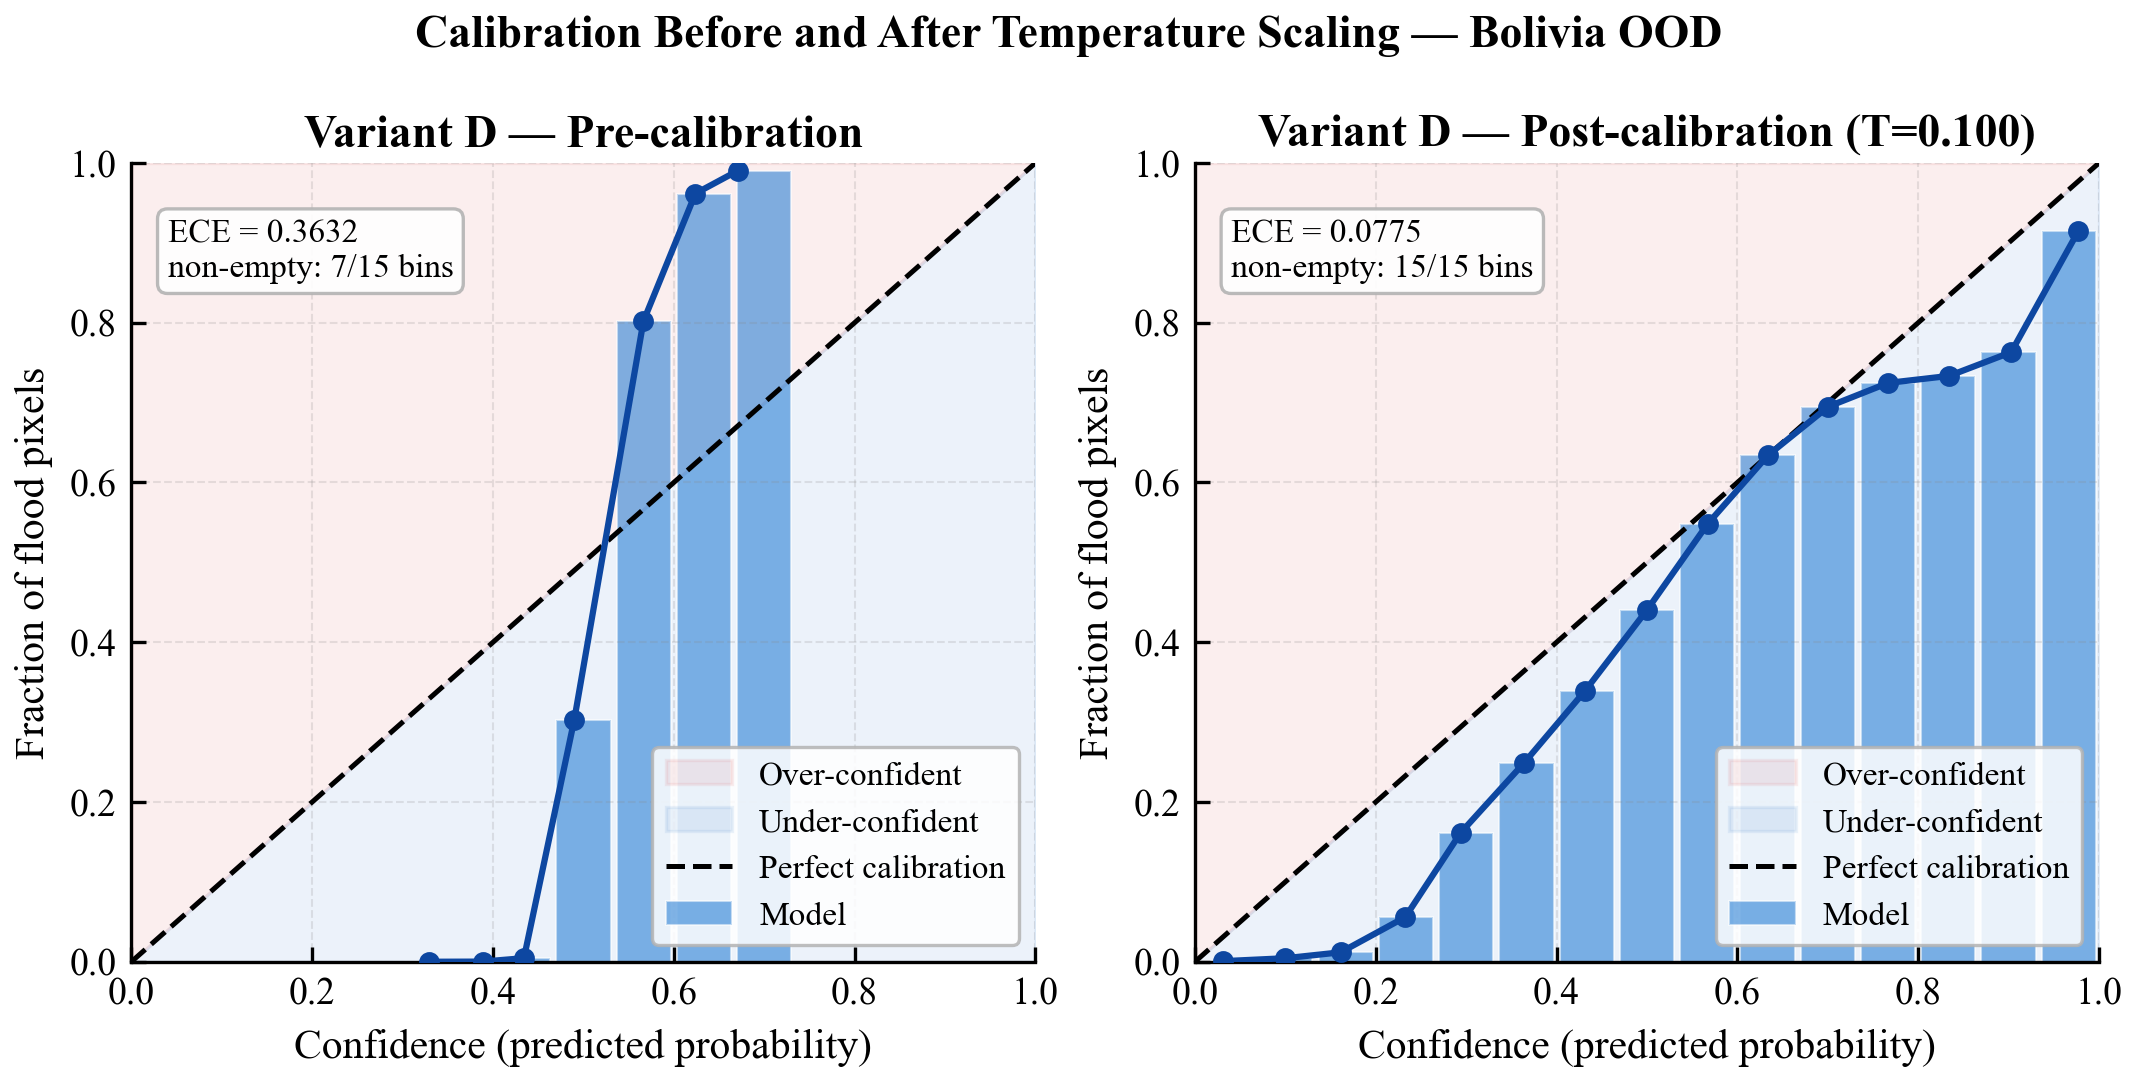
\includegraphics[width=0.90\textwidth]{fig_reliability_2panel}
\caption{Two-panel reliability diagram for Variant~D.
\textit{Left:} pre-calibration reliability curve showing severe underconfidence
(predicted probabilities cluster near 0.5).
\textit{Right:} post-calibration reliability curve ($T = 0.100$) showing
near-perfect alignment with the diagonal.
Both panels include the weighted average ECE and a confidence histogram.}
\label{fig:reliability_2panel}
\end{figure}

\begin{figure}[htbp]
\centering
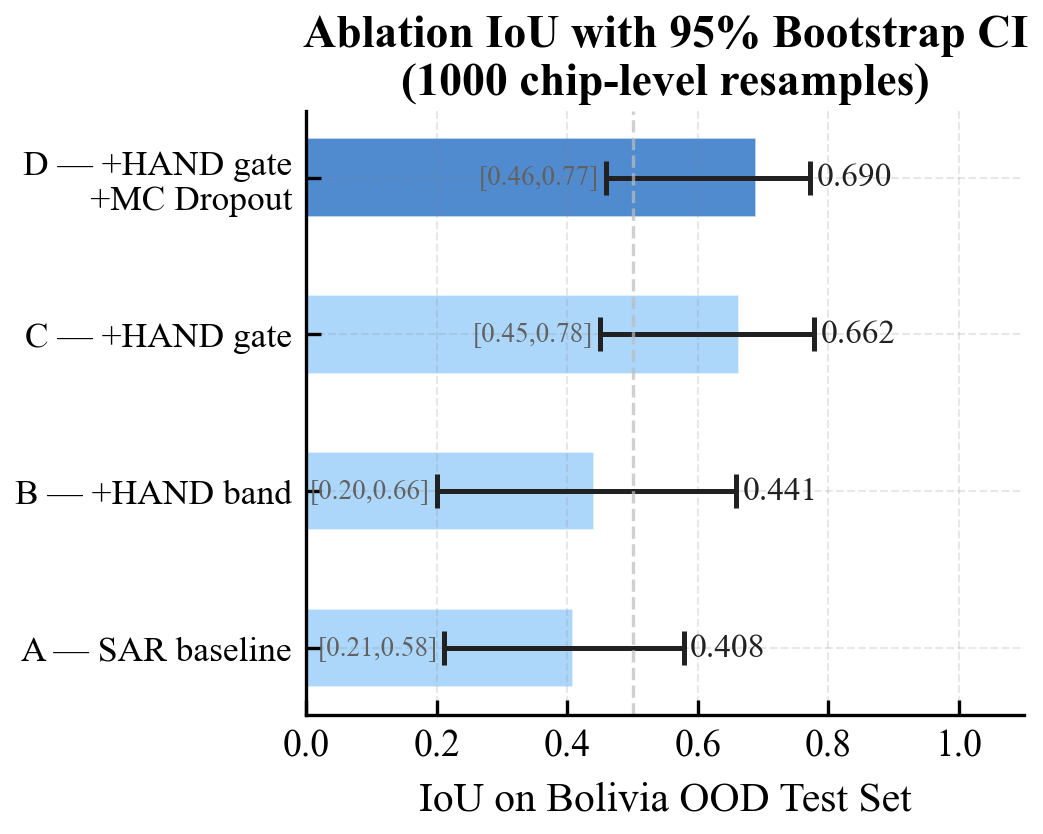
\includegraphics[width=0.80\textwidth]{fig_bootstrap_ci}
\caption{Bootstrap 95\% confidence intervals for the Bolivia test IoU of
Variants A, C, D, and D\_full (1{,}000 chip-level resamples).
The overlapping CIs for C and D illustrate the fundamental challenge of
evaluating on only 15 test chips.
The D\_full CI nominally dominates C, supporting the full-retraining
hypothesis.}
\label{fig:bootstrap_ci}
\end{figure}

\begin{figure}[htbp]
\centering
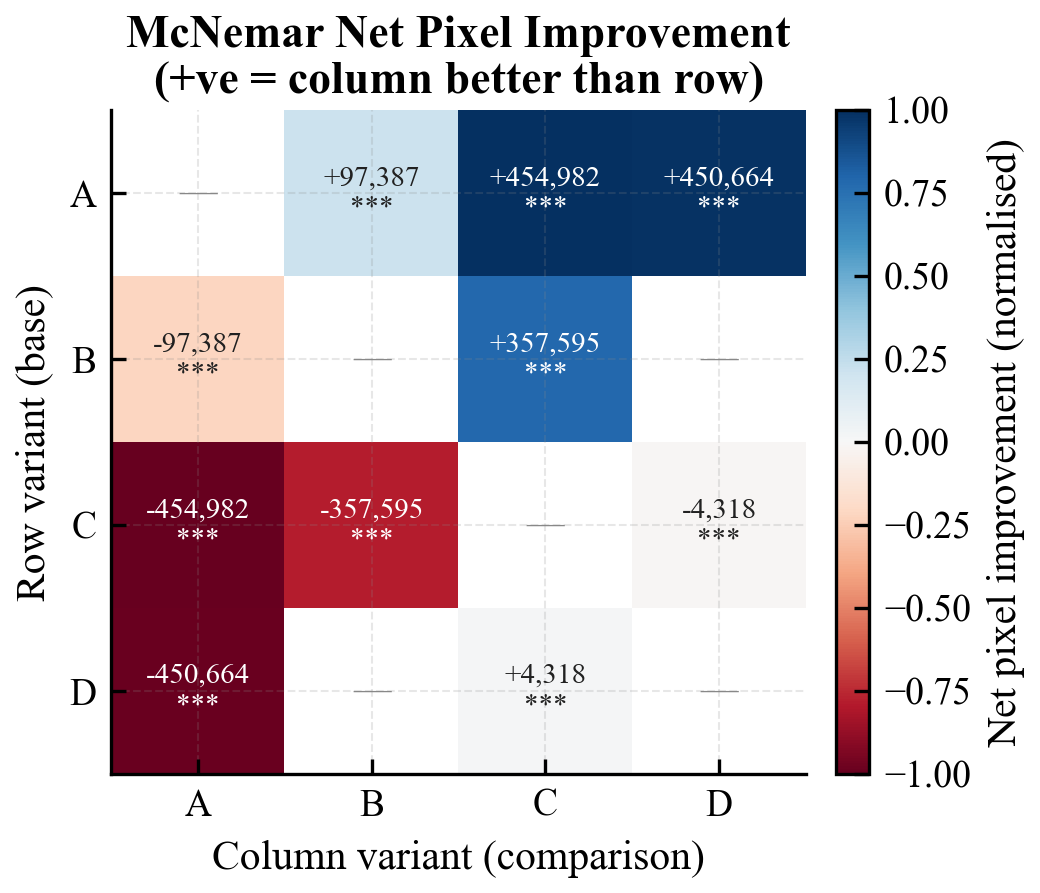
\includegraphics[width=0.80\textwidth]{fig_mcnemar}
\caption{McNemar test pixel-level comparison across all variant pairs
(heatmap of net correctly-classified pixel advantage).
All comparisons are highly significant ($p < 0.001$).
The C-vs-D comparison (highlighted) shows C marginally superior at the pixel
level ($\Delta = -4{,}318$ pixels) despite D's higher $\IoU$ ($+2.75$~pp),
illustrating the sensitivity of aggregate vs.\ per-pixel metrics to error
spatial structure.}
\label{fig:mcnemar}
\end{figure}

\begin{figure}[htbp]
\centering
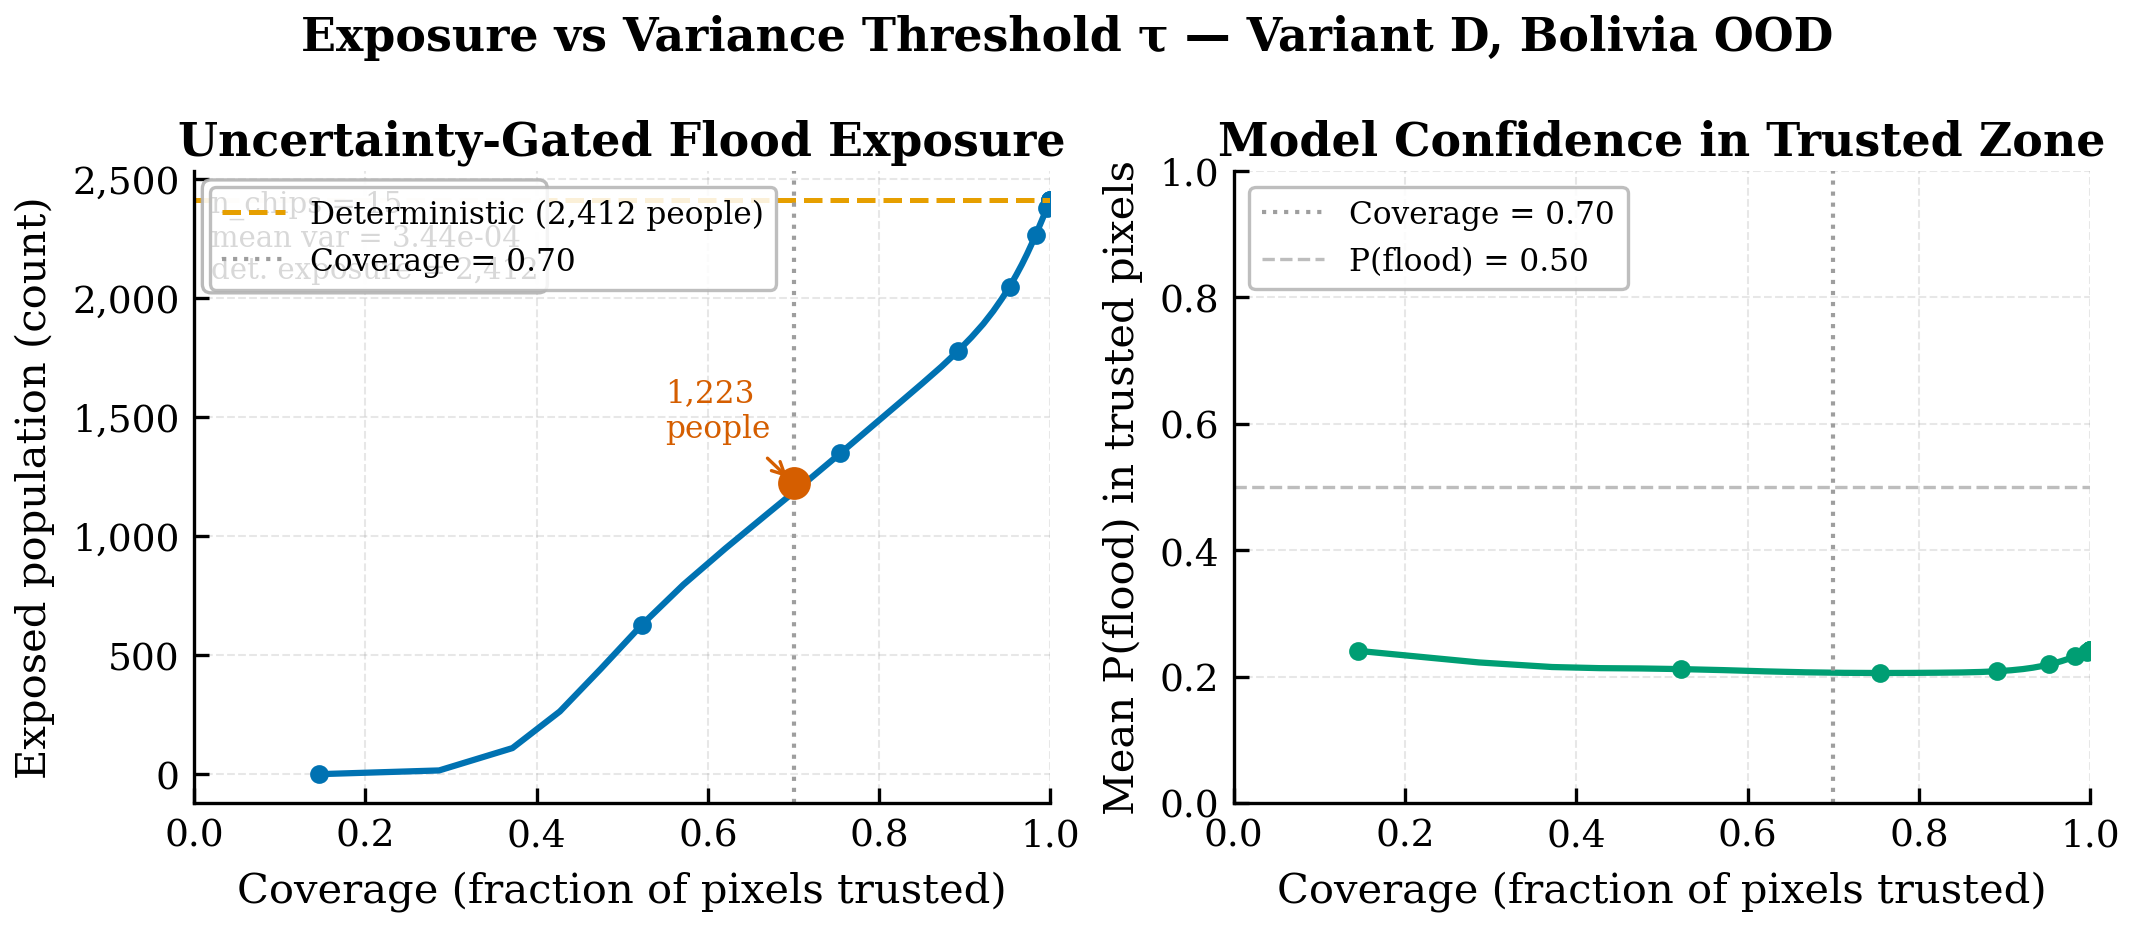
\includegraphics[width=0.80\textwidth]{fig_exposure_tau}
\caption{Sensitivity of population exposure to the uncertainty threshold
$\tau$ under TTA (solid line) and MC Dropout (dashed line).
TTA exposure decreases monotonically as $\tau$ tightens, indicating that
TTA variance provides effective uncertainty-based filtering.
MC Dropout exposure is flat across all $\tau \leq 0.05$, confirming that
MC variance falls entirely below any practically useful threshold.}
\label{fig:exposure_tau}
\end{figure}

\begin{figure}[htbp]
\centering
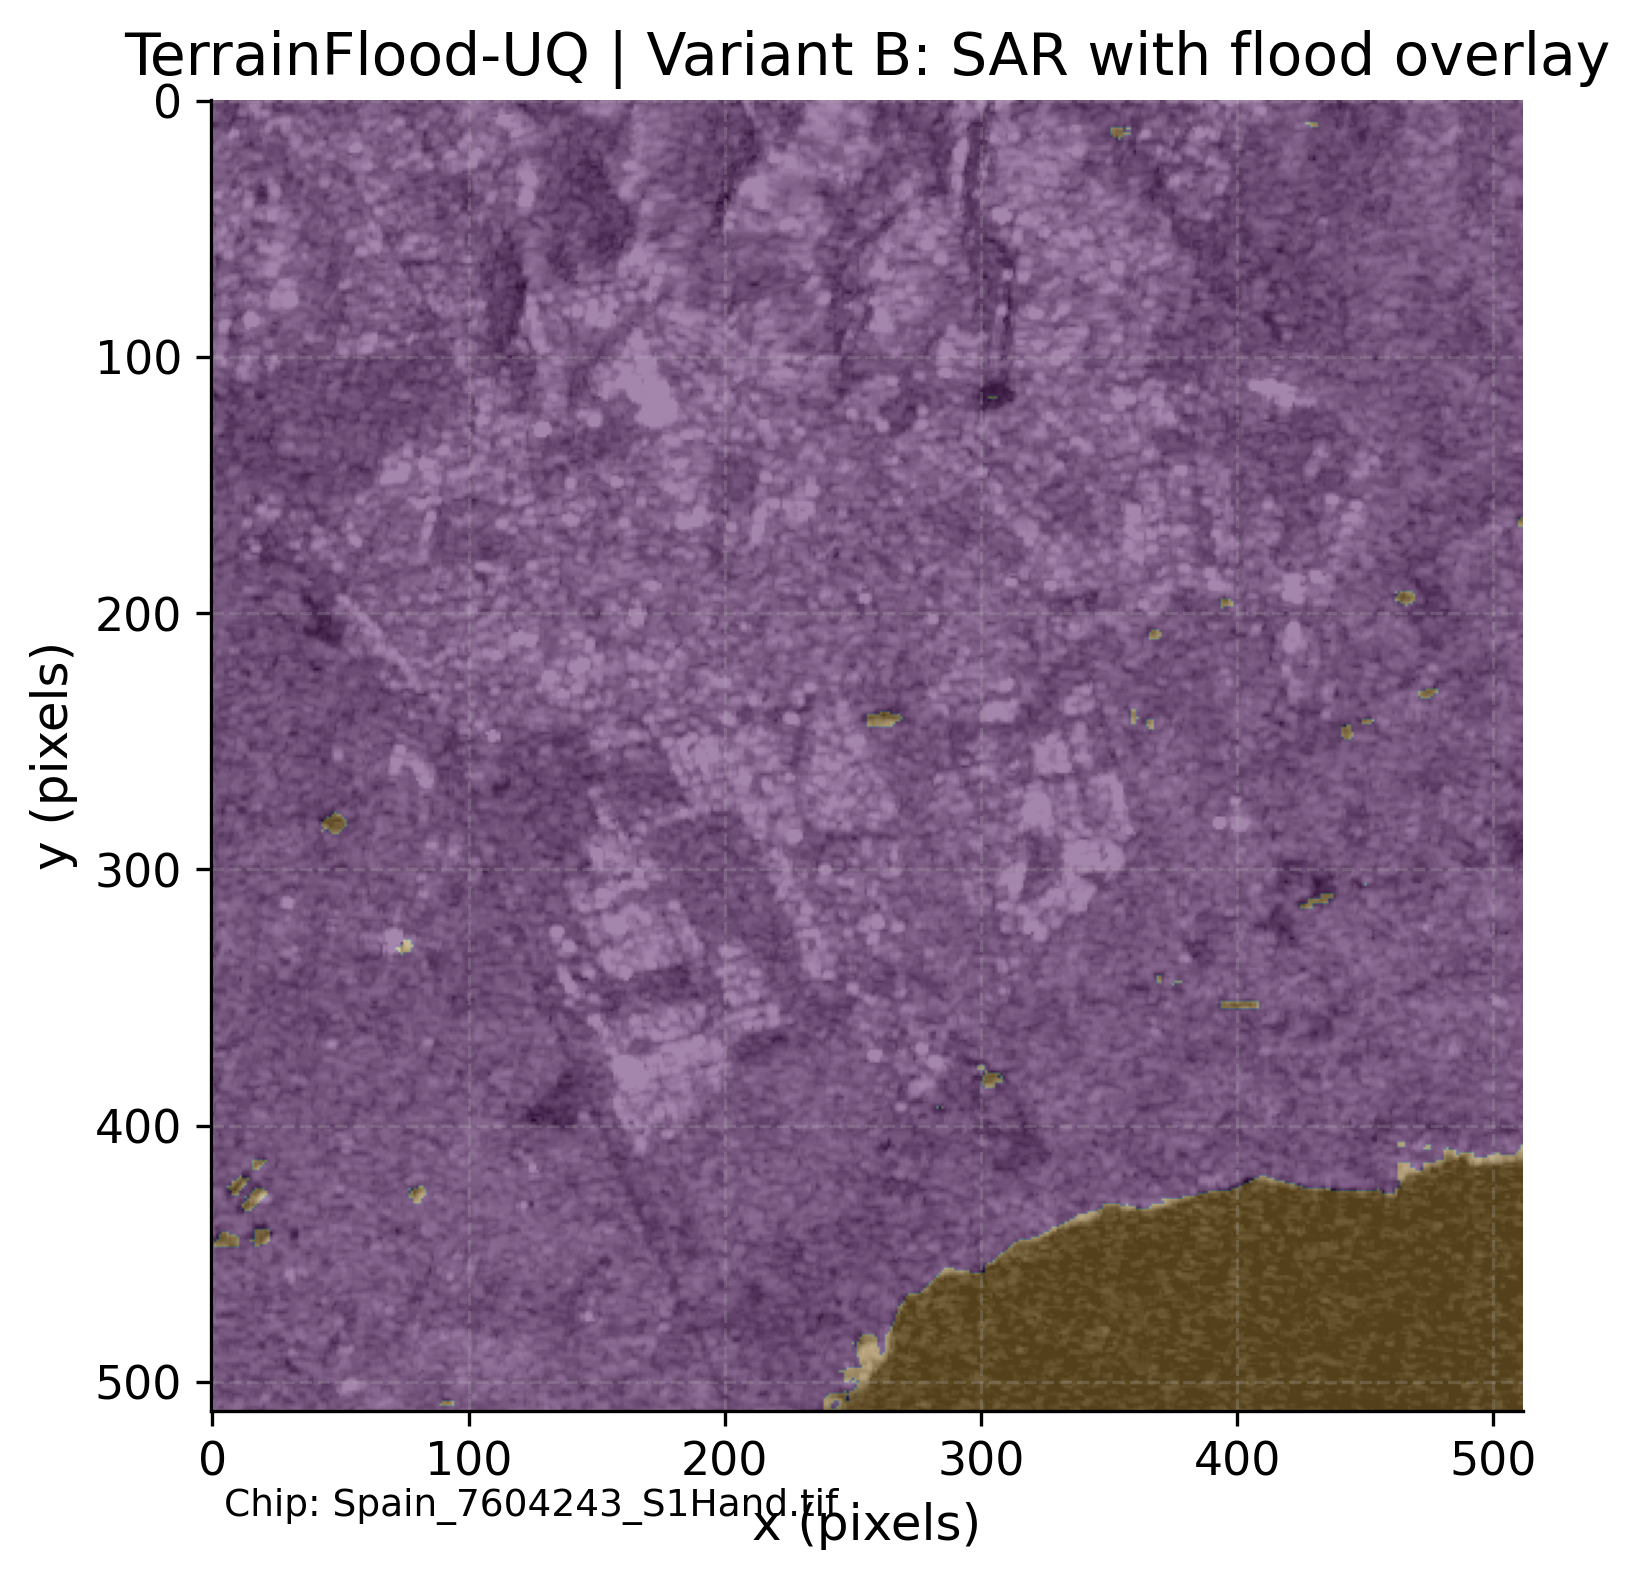
\includegraphics[width=0.95\textwidth]{figX_sar_label_overlay}
\caption{Sentinel-1 SAR with flood label overlay for multiple Bolivia test
chips.
Red contours indicate ground-truth flood boundaries; the grayscale background
shows VV post-event backscatter.
The strong correspondence between dark SAR pixels (specular reflection from
open water) and flood labels confirms data quality and motivates the
VV-based Otsu baseline.}
\label{fig:sar_overlay}
\end{figure}

%──────────────────────────────────────────────────────────────────────────────
\chapter{Repository Structure and Reproducibility}
\label{app:repo}
%──────────────────────────────────────────────────────────────────────────────

The complete codebase is available at
\url{https://github.com/Bouchra159/terrainflood}.
All results reported in this thesis were generated from the main branch at
commit \texttt{639fdaf}.
The repository is organised as follows:

\begin{verbatim}
terrainflood/
├── 01_gee_export.py       # GEE Sentinel-1 download (complete)
├── 02_dataset.py          # Sen1Floods11 dataset loader
├── 03_model.py            # Model variants A-E + HAND gate
├── train.py               # Training loop with early stopping
├── 05_uncertainty.py      # MC Dropout + TTA inference
├── 06_exposure.py         # WorldPop exposure analysis
├── eval.py                # Ablation evaluation + statistics
├── plots.py               # Figure generation
├── run_experiment.py      # End-to-end orchestration
├── jobs/                  # SLURM scripts for DKUCC
│   ├── train_A.sbatch ... train_D_full.sbatch
│   └── run_eval_all.sbatch, run_tta_uncertainty.sbatch
├── data/sen1floods11/
│   ├── norm_stats.json    # Normalisation statistics (CRITICAL)
│   └── HandLabeled/       # Sen1Floods11 chips
└── results/               # All experimental outputs (pushed to GitHub)
    ├── ablation/          # Ablation comparison
    ├── eval_A/ ... eval_D_full/ # Per-variant evaluation
    ├── uncertainty_D/     # MC Dropout UQ results
    ├── uncertainty_tta/   # TTA UQ results
    ├── exposure_D_full/   # Population exposure
    └── paper_figures/     # Publication-ready figures
\end{verbatim}

To reproduce the full pipeline:
\begin{enumerate}
  \item Clone the repository and install dependencies:
        \texttt{pip install -r requirements.txt}
  \item Download Sen1Floods11 hand-labelled chips to
        \texttt{data/sen1floods11/HandLabeled/}
  \item Submit training jobs:
        \texttt{sbatch jobs/train\_D\_full.sbatch}
  \item After training, run evaluation:
        \texttt{sbatch jobs/run\_eval\_all.sbatch}
  \item Run TTA uncertainty:
        \texttt{sbatch jobs/run\_tta\_uncertainty.sbatch}
\end{enumerate}

All training configurations are fully specified in the SLURM job scripts.
CUDA, PyTorch, and Rasterio must be installed at the system level;
see \texttt{jobs/train\_D\_full.sbatch} for the module-load commands used on
DKUCC.

\end{document}
